
% ----------------------------------------------------------------------
%                   LATEX TEMPLATE FOR PhD THESIS
% ----------------------------------------------------------------------

% based on Harish Bhanderi's PhD/MPhil template, then Uni Cambridge
% http://www-h.eng.cam.ac.uk/help/tpl/textprocessing/ThesisStyle/
% corrected and extended in 2007 by Jakob Suckale, then MPI-CBG PhD programme
% and made available through OpenWetWare.org - the free biology wiki


%: Style file for Latex
% Most style definitions are in the external file PhDthesisPSnPDF.
% In this template package, it can be found in ./Latex/Classes/
\documentclass[twoside,11pt]{Latex/Classes/PhDthesisPSnPDF}

%: Macro file for Latex
% Macros help you summarise frequently repeated Latex commands.
% Here, they are placed in an external file /Latex/Macros/MacroFile1.tex
% An macro that you may use frequently is the figuremacro (see introduction.tex)
% This file contains macros that can be called up from connected TeX files
% It helps to summarise repeated code, e.g. figure insertion (see below).

% todo macro
\usepackage{color}
\newcommand{\todo}[1]{\noindent\textcolor{red}{{\bf \{TODO}: #1{\bf \}}}}

\usepackage{xspace}
\newcommand{\googleplus}{Google\nolinebreak\hspace{0em}\raisebox{.28ex}{\tiny\bf +}\kern-0.2ex\xspace}

% insert a centered figure with caption and description
% parameters 1:filename, 2:title, 3:description and label
\newcommand{\figuremacro}[3]{
	\begin{figure}[htbp]
		\centering
		\includegraphics[width=1\textwidth]{#1}
		\caption[#2]{\textbf{#2} - #3}
		\label{fig:#1}
	\end{figure}
}

% insert a centered figure with caption and description AND WIDTH
% parameters 1:filename, 2:title, 3:description and label, 4: textwidth
% textwidth 1 means as text, 0.5 means half the width of the text
\newcommand{\figuremacroW}[4]{
	\begin{figure}[htbp]
		\centering
		\includegraphics[width=#4\textwidth]{#1}
		\caption[#2]{\textbf{#2} - #3}
		\label{fig:#1}
	\end{figure}
}

% inserts a figure with wrapped around text; only suitable for NARROW figs
% o is for outside on a double paged document; others: l, r, i(inside)
% text and figure will each be half of the document width
% note: long captions often crash with adjacent content; take care
% in general: above 2 macro produce more reliable layout
\newcommand{\figuremacroN}[3]{
	\begin{wrapfigure}{o}{0.5\textwidth}
		\centering
		\includegraphics[width=0.48\textwidth]{#1}
		\caption[#2]{{\small\textbf{#2} - #3}}
		\label{fig:#1}
	\end{wrapfigure}
}

% predefined commands by Harish
\newcommand{\PdfPsText}[2]{
  \ifpdf
     #1
  \else
     #2
  \fi
}

\newcommand{\IncludeGraphicsH}[3]{
  \PdfPsText{\includegraphics[height=#2]{#1}}{\includegraphics[bb = #3, height=#2]{#1}}
}

\newcommand{\IncludeGraphicsW}[3]{
  \PdfPsText{\includegraphics[width=#2]{#1}}{\includegraphics[bb = #3, width=#2]{#1}}
}

\newcommand{\InsertFig}[3]{
  \begin{figure}[!htbp]
    \begin{center}
      \leavevmode
      #1
      \caption{#2}
      \label{#3}
    \end{center}
  \end{figure}
}


%%% Local Variables: 
%%% mode: latex
%%% TeX-master: "~/Documents/LaTeX/CUEDThesisPSnPDF/thesis"
%%% End: 




%: ----------------------------------------------------------------------
%:                  TITLE PAGE: name, degree,..
% ----------------------------------------------------------------------
% below is to generate the title page with crest and author name

%if output to PDF then put the following in PDF header
\ifpdf  
    \pdfinfo { /Title  (PhD and MPhil Thesis Classes)
               /Creator (TeX)
               /Producer (pdfTeX)
               /Author (YourName your@email.net)
               /CreationDate (D:YYYYMMDDhhmmss)  %format D:YYYYMMDDhhmmss
               /ModDate (D:YYYYMMDDhhmm)
               /Subject (xyz)
               /Keywords (add, your, keywords, here) }
    \pdfcatalog { /PageMode (/UseOutlines)
                  /OpenAction (fitbh)  }
\fi


\title{Enriching unstructured media content about events to enable semi-automated summaries, compilations, and improved search by leveraging social networks}



% ----------------------------------------------------------------------
% The section below defines www links/email for author and institutions
% They will appear on the title page of the PDF and can be clicked
\ifpdf
  \author{\href{mailto:tsteiner@lsi.upc.edu}{Thomas Steiner}}
%  \cityofbirth{born in XYZ} % uncomment this if your university requires this
%  % If city of birth is required, also uncomment 2 sections in PhDthesisPSnPDF
%  % Just search for the "city" and you'll find them.
  \collegeordept{\href{http://www.lsi.upc.edu/}{Departament de Llenguatges i Sistemes Informàtics}}
  \university{\href{http://www.upc.edu/}{Universitat Politècnica de Catalunya}}

  % The crest is a graphics file of the logo of your research institution.
  % Place it in ./frontmatter/figures and specify the width
  \crest{
\includegraphics[width=4cm]{upc-logo}}
  
% If you are not creating a PDF then use the following. The default is PDF.
\else
  \author{Thomas Steiner}
%  \cityofbirth{born in XYZ}
  \collegeordept{Departament de Llenguatges i Sistemes Informàtics}
  \university{Universitat Politècnica de Catalunya}
  \crest{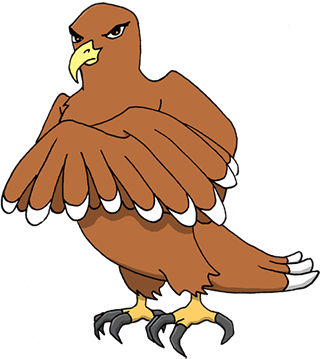
\includegraphics[width=4cm]{logo}}
\fi

%\renewcommand{\submittedtext}{change the default text here if needed}
\degree{Philosophi{\ae} Doctor (PhD)}
\degreedate{December 2012}


% ----------------------------------------------------------------------
       
% turn of those nasty overfull and underfull hboxes
\hbadness=10000
\hfuzz=50pt


%: --------------------------------------------------------------
%:                  FRONT MATTER: dedications, abstract,..
% --------------------------------------------------------------

\begin{document}

%\language{english}

% sets line spacing
\renewcommand\baselinestretch{1.2}
\baselineskip=18pt plus1pt


%: ----------------------- generate cover page ------------------------

\maketitle  % command to print the title page with above variables


%: ----------------------- cover page back side ------------------------
% Your research institution may require reviewer names, etc.
% This cover back side is required by Dresden Med Fac; uncomment if needed.

\newpage
\vspace{10mm}
1. Reviewer: Joaquim Gabarró Vallés (UPC)

\vspace{10mm}
2. Reviewer: Michael Hausenblas (DERI)

\vspace{20mm}
Day of the defense: \todo{add date of the defense}

\vspace{20mm}
\hspace{70mm}Signature from head of PhD committee:



%: ----------------------- abstract ------------------------

% Your institution may have specific regulations if you need an abstract and where it is to be placed in the document. The default here is just after title.

\begin{abstracts}

\textbf{(i) Mobile devices and social networks are omnipresent}

Mobile devices such as smartphones, tablets, or digital cameras
together with social networks enable people to create,
share, and consume enormous amounts of media items
like videos or photos both on the road or at home.
Such mobile devices---by pure definition---accompany
their owners almost wherever they may go.
In consequence, mobile devices are omnipresent
at all sorts of events to capture noteworthy moments.
Exemplary events can be keynote speeches at conferences,
music concerts in stadiums,
or even natural catastrophes like earthquakes
that affect whole areas or countries.
At such events---given a~stable network connection---part of
the event-related media items are published on social networks
both as the event happens or afterwards,
once a~stable network connection has been established again.

\textbf{(ii) Finding representative media items
for an event is hard}

Common media item search operations,
for example, searching for \emph{the} official video clip
for a~certain hit record on an online video platform
can in the simplest case be achieved based on potentially
shallow human-generated metadata
or based on more profound content analysis techniques
like optical character recognition,
automatic speech recognition,
or acoustic fingerprinting.
More advanced scenarios, however, like retrieving all
(or just the most representative) media items
that were created at a~given event
with the objective of creating \emph{event summaries} or
\emph{media item compilations} covering the event in question
are hard, if not impossible, to fulfill at large scale.
The main research question of this thesis
can be formulated as follows.

\textbf{(iii) Research question}

\textit{``Can user-customizable media galleries
that summarize given events be\linebreak
created solely based on textual and multimedia data
from social networks?''}

\textbf{(iv) Contributions}

In the context of this thesis, we have developed and evaluated
a~novel interactive application and related methods
for media item enrichment,
leveraging social networks, utilizing the Web of Data,
techniques known from Content-based Image Retrieval~(CBIR)
and Content-based Video Retrieval~(CBVR),
and fine-grained media item addressing schemes
like Media Fragments URIs
to provide a~scalable and near realtime solution
to realize the abovementioned scenario
of event summarization and media item compilation.

\textbf{(v) Methodology}

For any event with given event title(s),
(potentially vague) event location(s), and
(arbitrarily fine-grained) event date(s),
our approach can be divided in the following six steps.

\begin{enumerate}
  \item Via the textual search APIs (Application Programming Interfaces) of
        different social networks,
        we retrieve a~list of potentially event-relevant
        microposts that either contain media items directly,
        or that provide links to media items
        on external media item hosting platforms.
  \item Using third-party
        Natural Language Processing (NLP) tools,
        we recognize and disambiguate named entities
        in microposts to predetermine their relevance.
  \item We extract the binary media item data
        from social networks or media item hosting platforms
        and relate it to the originating microposts.
  \item Using CBIR and CBVR techniques, we first deduplicate
        exact-duplicate and near-duplicate media items
        and then cluster similar media items.
  \item We rank the deduplicated and clustered list
        of media items and their related microposts
        according to well-defined ranking criteria.
  \item In order to generate interactive and user-customizable
        media galleries that visually and audially summarize the
        event in question, we compile the top-$n$ ranked
        media items and microposts in aesthetically pleasing
        and functional ways.
\end{enumerate}
\end{abstracts}


% The original template provides and abstractseparate environment, if your institution requires them to be separate. I think it's easier to print the abstract from the complete thesis by restricting printing to the relevant page.
% \begin{abstractseparate}
%   \begin{abstracts}

\textbf{(i) Mobile devices and social networks are omnipresent}

Mobile devices such as smartphones, tablets, or digital cameras
together with social networks enable people to create,
share, and consume enormous amounts of media items
like videos or photos both on the road or at home.
Such mobile devices---by pure definition---accompany
their owners almost wherever they may go.
In consequence, mobile devices are omnipresent
at all sorts of events to capture noteworthy moments.
Exemplary events can be keynote speeches at conferences,
music concerts in stadiums,
or even natural catastrophes like earthquakes
that affect whole areas or countries.
At such events---given a~stable network connection---part of
the event-related media items are published on social networks
both as the event happens or afterwards,
once a~stable network connection has been established again.

\textbf{(ii) Finding representative media items
for an event is hard}

Common media item search operations,
for example, searching for \emph{the} official video clip
for a~certain hit record on an online video platform
can in the simplest case be achieved based on potentially
shallow human-generated metadata
or based on more profound content analysis techniques
like optical character recognition,
automatic speech recognition,
or acoustic fingerprinting.
More advanced scenarios, however, like retrieving all
(or just the most representative) media items
that were created at a~given event
with the objective of creating \emph{event summaries} or
\emph{media item compilations} covering the event in question
are hard, if not impossible, to fulfill at large scale.
The main research question of this thesis
can be formulated as follows.

\textbf{(iii) Research question}

\textit{``Can user-customizable media galleries
that summarize given events be\linebreak
created solely based on textual and multimedia data
from social networks?''}

\textbf{(iv) Contributions}

In the context of this thesis, we have developed and evaluated
a~novel interactive application and related methods
for media item enrichment,
leveraging social networks, utilizing the Web of Data,
techniques known from Content-based Image Retrieval~(CBIR)
and Content-based Video Retrieval~(CBVR),
and fine-grained media item addressing schemes
like Media Fragments URIs
to provide a~scalable and near realtime solution
to realize the abovementioned scenario
of event summarization and media item compilation.

\textbf{(v) Methodology}

For any event with given event title(s),
(potentially vague) event location(s), and
(arbitrarily fine-grained) event date(s),
our approach can be divided in the following six steps.

\begin{enumerate}
  \item Via the textual search APIs (Application Programming Interfaces) of
        different social networks,
        we retrieve a~list of potentially event-relevant
        microposts that either contain media items directly,
        or that provide links to media items
        on external media item hosting platforms.
  \item Using third-party
        Natural Language Processing (NLP) tools,
        we recognize and disambiguate named entities
        in microposts to predetermine their relevance.
  \item We extract the binary media item data
        from social networks or media item hosting platforms
        and relate it to the originating microposts.
  \item Using CBIR and CBVR techniques, we first deduplicate
        exact-duplicate and near-duplicate media items
        and then cluster similar media items.
  \item We rank the deduplicated and clustered list
        of media items and their related microposts
        according to well-defined ranking criteria.
  \item In order to generate interactive and user-customizable
        media galleries that visually and audially summarize the
        event in question, we compile the top-$n$ ranked
        media items and microposts in aesthetically pleasing
        and functional ways.
\end{enumerate}
\end{abstracts}

% \end{abstractseparate}


%: ----------------------- tie in front matter ------------------------

\frontmatter
\begin{dedication} %this creates the heading for the dedication page
To Laura, Lena, Emma, and Nil.
\end{dedication}

\begin{acknowledgements}

\textbf{Personal Acknowledgements:}

First and foremost, I~would like to thank my wife Laura
for her support, understanding, patience, and energy
during my time as a~PhD student, and simply for being at my side.
Without you, I~would not be where I~am today.

I~wholeheartedly thank my two advisors Joaquim Gabarró Vallés
and Michael Hausenblas for their guidance, helpful comments,
informative pointers, and especially
for their constructive criticisms.
The areas of research that I~have tackled in this thesis
are still young and sometimes uncharted territory.
I~am very thankful that the two of you have ventured
on the undertaking of leading me through this thesis.

I~deeply appreciate all the review comments, thoughts, challenging questions,
and, last not least, the \LaTeX~help of my dear friend
and research colleague Ruben Verborgh.
It was, is, and will be an honor to work with you.
My warm thanks also go to Raphaël Troncy and his team
at \mbox{EURECOM} Sophia Antipolis in France
who have helped shape some of the ideas presented in this thesis.

I~would like to thank my former and current managers at Google,
namely N.~Kryvossidis, R.~Ashley, C.~Bouchère, and I.~Sassarini
for their support for my thesis.
A~lot of valuable input for my thesis came in via social networks.
My thanks go out to everyone I have interacted with
around the hashtag \texttt{\#TomsPhD}
on Twitter, \googleplus, and Facebook.

Finally, I~sincerely thank my parents and my brother
who have made me the person I~am today.
My parents have taught me
not to go for the easy choices, even
if at times they may seem tempting,
but instead to try harder and never give up.
This thesis also is for you.

\textbf{Formal Acknowledgements:}

The research presented in this thesis
was partially supported by the European Commission
under Grant No. 248296 with the European Union (FP7 ICT STReP)
project \mbox{\emph{I-SEARCH}}.

\vspace{80mm}

\textbf{To cite this document:}

\small
\begin{verbatim}
  @phdthesis{steiner2013thesis,
    author = {Thomas Steiner},
    title  = {Enriching Unstructured Media Content About Events to
              Enable Semi-Automated Summaries, Compilations, and
              Improved Search by Leveraging Social Networks},
    year   = {2013},
    school = {Universitat Polit\`{e}cnica de Catalunya}
  }
\end{verbatim}

\normalsize

\vspace{10mm}
\textbf{Copyright and License:}\\\\
\small \copyright \normalsize 2013 Thomas Steiner\\
Licensed under the Creative Commons Attribution-ShareAlike 3.0 License.\\
\url{http://creativecommons.org/licenses/by-sa/3.0/}

\end{acknowledgements}



%: ----------------------- contents ------------------------

\setcounter{secnumdepth}{3} % organisational level that receives a numbers
\setcounter{tocdepth}{3}    % print table of contents for level 3
\tableofcontents            % print the table of contents
% levels are: 0 - chapter, 1 - section, 2 - subsection, 3 - subsection


%: ----------------------- list of figures/tables ------------------------

\listoffigures	% print list of figures

\listoftables  % print list of tables


%: ----------------------- glossary ------------------------

% Tie in external source file for definitions: /frontmatter/glossary.tex
% Glossary entries can also be defined in the main text. See glossary.tex
% this file is called up by thesis.tex
% content in this file will be fed into the main document

% Glossary entries are defined with the command \nomenclature{1}{2}
% 1 = Entry name, e.g. abbreviation; 2 = Explanation
% You can place all explanations in this separate file or declare them in the middle of the text. Either way they will be collected in the glossary.

% required to print nomenclature name to page header
\markboth{\MakeUppercase{\nomname}}{\MakeUppercase{\nomname}}

\nomenclature{NLP}{Natural Language Processing}
\nomenclature{CBIR}{Content-based Image Retrieval} 
\nomenclature{CBVR}{Content-based Video Retrieval} 
\nomenclature{RDF}{Resource Description Framework}
\nomenclature{W3}{World-Wide Web}
\nomenclature{WWW}{World-Wide Web}
\nomenclature{CERN}{European Organization for Nuclear Research}
\nomenclature{HTML}{Hypertext Markup Language}
\nomenclature{URI}{Unique Resource Identifier}
\nomenclature{URL}{Unique Resource Locator}
\nomenclature{JSON}{JavaScript Object Notation}
\nomenclature{Turtle}{Terse RDF Triple Language}
\nomenclature{CURIE}{Compact URI}
\nomenclature{SPARQL}{SPARQL Protocol and RDF Query Language}
\nomenclature{W3C}{World Wide Web Consortium}
\nomenclature{LOD}{Linking Open Data}
\nomenclature{SNS}{Social Network(ing) Site}
\nomenclature{API}{Application Programming Interface}
\nomenclature{NEE}{Named Entity Extraction}
\nomenclature{NER}{Named Entity Recognition}
\nomenclature{OWL}{Web Ontology Language}
\nomenclature{DOM}{Document Object Model}
\nomenclature{POS}{Part-of-Speech (tagging)} 

\begin{multicols}{2} % \begin{multicols}{#columns}[header text][space]
\begin{footnotesize} % scriptsize(7) < footnotesize(8) < small (9) < normal (10)

\printnomenclature[1.5cm] % [] = distance between entry and description
\label{nom} % target name for links to glossary

\end{footnotesize}
\end{multicols}



%: --------------------------------------------------------------
%:                  MAIN DOCUMENT SECTION
% --------------------------------------------------------------

% the main text starts here with the introduction, 1st chapter,...
\mainmatter

\renewcommand{\chaptername}{} % uncomment to print only "1" not "Chapter 1"
\renewcommand\chapterautorefname{Chapter}

%: ----------------------- subdocuments ------------------------

% Parts of the thesis are included below. Rename the files as required.
% But take care that the paths match. You can also change the order of appearance by moving the include commands.

\chapter{Event Summarization Challenge}
\label{cha:introduction}

% the code below specifies where the figures are stored
\ifpdf
    \graphicspath{{1_introduction/figures/PNG/}{1_introduction/figures/PDF/}{1_introduction/figures/}}
\else
    \graphicspath{{1_introduction/figures/EPS/}{1_introduction/figures/}}
\fi

\section{Motivation and Problem Statement}

A~very open definition of the word \emph{event}
given by WordNet~\cite{fellbaum1998wordnet,miller1995wordnet} is
\emph{``something that happens at a~given place and time''}.
Following this definition,
we are indeed surrounded by events,
most of which are of little to no interest for us.
A~concert somewhere in the world of a~band
that we do not even know may be a~good example.
For some events, however, we may care more, for example,
a~concert of a~band that we know and like,
even if it takes place at a~location far away from us.
Finally, for very few events, we may care a~lot,
maybe even enough to physically attend the event,
like a~concert of our favorite band
if it takes place in our city, is not sold out,
and not too expensive.

All this motivates the need for \emph{event summarization}.
If there is an event that we could not attend
for any given reason,
but that we are interested in,
a~good event summarization can help us get a~feeling
for the event's atmosphere.
Similarly, if there is an event that we attended,
we can revive the event's most fascinating moments
based on the event summarization.

A~\emph{media gallery} in the context of
our event summarization task is
a~\emph{best-of} compilation of photos, videos,
and microposts retrieved from social networks
that are related to a~given event.
Event summarization covers textual
as well as multimedia content.
We say a~media gallery is of high quality,
if it fulfills the following properties.

\begin{enumerate}
  \item \textit{Conciseness:}
        it conveys a~lot of information clearly
        and in few media items.
  \item \textit{Comprehensiveness:}
        it is complete and covers all representative
        elements or aspects of an event.
  \item \textit{Authenticity:}
        it is of undisputed origin and genuine.
  \item \textit{Diversity:}
        it shows a~great deal of variety.
  \item \textit{Interestingness:}
        it catches and holds the attention of the viewer.     
\end{enumerate}

\section{Research Question and Hypothesis}

The main research question for this thesis
can be formulated as follows.
 
\textit{``Can user-customizable
media galleries that summarize given events be
created solely based on textual and multimedia data
from social networks?''}

\noindent The hypothesis that we test in this thesis
can be formulated as follows.

We argue that through media galleries that leverage content
that was shared on social networks,
a~more \emph{authentic}, more \emph{concise},
more \emph{comprehensive}, more \emph{diverse},
and also more \emph{interesting}
view on events gets possible than by limiting oneself
to officially produced media content;
and that further such media galleries can be generated
more \emph{efficiently} and \emph{in shorter time}
than manually produced media galleries.

We validate these subjective and objective
criteria with experiments for events of different categories
such as sports, politics, culture, leisure,
music, conferences, \emph{etc.}

\section{Approach}

The objective of this thesis is the development
of methods for the automated summarization of events
based on media items shared on social networks.
A~schematic overview of the approach can be seen
in~\autoref{fig:thesis-diagram}.
As an event takes places and shortly thereafter
(symbolized by the timeline marked with \emph{2h Event}),
people share media items related to the event
on multiple social networks
(symbolized by the photo and video pictograms
above the event timeline).
Via the textual search APIs (Application Programming Interfaces)
of these different social networks,
we retrieve a~list of potentially event-relevant
microposts that either contain media items directly,
or that provide links to media items
on external media item hosting platforms.
Using third-party NLP tools,
we recognize and disambiguate named entities
in the microposts to predetermine their relevance.
We extract the binary media item data
from social networks or media item hosting platforms
and relate it to the originating microposts
(symbolized by the central cloud).
Using CBIR and CBVR techniques, we first deduplicate
duplicate and near-duplicate media items,
and then cluster similar media items
(symbolized by the green, red, and orange markers).
We rank the deduplicated and clustered list
of media items and their related microposts
according to well-defined ranking criteria.
In order to generate interactive and user-customizable
media galleries that visually and audially summarize the
event in question, we compile the top-$n$ ranked
media items and microposts in an aesthetic way
(symbolized by the timeline marked with \emph{5min Summary}).

\begin{figure}[!ht]
  \centering
  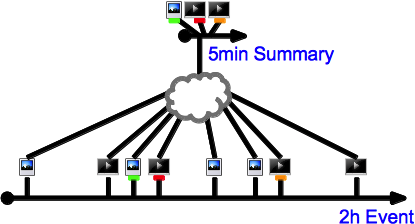
\includegraphics[]{thesis-diagram.png}
  \caption[Schematic depiction of event summary generation]
    {Schematic depiction of event summary generation
    based on deduplicated, clustered, and ranked media items
    for an exemplary event}
  \label{fig:thesis-diagram}
\end{figure}

\section{Contributions}

In this thesis, we report on methods for
the automated generation of event summaries.
This particular field of research touches on many related areas
of research and research communities,
amongst which social network research, multimedia content analysis,
Semantic Web and Natural Language Processing (NLP),
human factors in computing systems,
and Web services.
Early on in the process of this thesis,
we have sought and incorporated expert feedback based on
a~Doctoral Consortium paper~%
\cite{steiner2011enrichingunstructured}.
We have broken our contributions down into
the following topics.

\subsection{Social Network Multimedia and Data Analysis}

We have worked on methods for the aggregation, extraction,
deduplication, clustering, and compilation
of social media contents from
multiple social networks~%
\cite{rizzo2012whatfresh}.
Those methods were applied and evaluated
for the enhancement of conference experiences~%
\cite{khrouf2012aggregatingsocialmedia,khrouf2012confomaton}.

\subsection{Application of Semantic Web and NLP Techniques}

In order to make sense out of social network microposts,
we have worked on methods to consolidate and rank
the results of multiple named entity recognition and
disambiguation APIs and to track their data provenance~%
\cite{steiner2011addingmeaning}.
We have applied and evaluated those methods
for the consumer-oriented detection of trending microposts
on a~major commercial social network~%
\cite{steiner2011tweetconsumers}.


\subsection{Video Content and Metadata Analysis}

We have worked on methods for named entity extraction and
disambiguation for online videos based on closed captions
and other textual metadata, which make online video
more accessible, searchable, and interconnected~%
\cite{steiner2010semwebvid,steiner2010semwebvidchallenge}.
Further, we have combined those textual methods with 
video content analysis methods for the on-the-fly detection
of shot boundaries for online videos~%
\cite{steiner2012shotdetection}.
We have defined aesthetic principles
for the automated generation of media gallery layouts
for visual and audial event summarization
based on social network multimedia data~%
\cite{steiner2012definingaesthetic}.
        
\subsection{Crowdsourcing}

The video content analysis methods mentioned before
were combined with methods for the crowdsourced detection
of events in online videos~%
\cite{steiner2011crowdsourcingevent}.
We have further worked on crowdsourcing methods
for the extraction of knowledge items from arbitrary Web pages~%
\cite{steiner2012sekiathome,steiner2012sekiathomechallenge}.

\subsection{Studies}

We have contributed an examination of Linked Data usage and
visualization techniques of a~major commercial search engine~%
\cite{steiner2010howgoogleisusing}.
In addition to that, we have studied the usefulness and relevance
of social network updates which were added to search engine
results pages (SERP) of a~major commercial search engine~%
\cite{steiner2012addingrealtime}.

\subsection{Multimodal Search Engines}

We have worked on an examination of context-aware querying
for multimodal search engines~%
\cite{etzold2012contextawarequerying,steiner2012isearch}.
Further, we have studied user interface constraints on
mobile and desktop devices for a~multimodal search engine
and demonstrated that those constraints can be overcome~%
\cite{steiner2012onesizedoesnotfitall}.


\subsection{Web Service Description}

We have worked on methods for the semantic description of Web APIs,
their discoverability, their automated consumption,
their semantic interlinking, and their social aspects~%
\cite{verborgh2011descriptionandinteraction,verborgh2011efficientruntime,verborgh2011integratingdata,verborgh2012capturingthefunctionality,verborgh2012functionalcomposition,verborgh2012functionaldescriptions,verborgh2012missinglinks,verborgh2012restdesc,verborgh2012socialdescriptionrevolution}.
We have studied the feasibility of truly RESTful behavior
for Web APIs in the sense of Dr. Roy Fielding~%
\cite{steiner2011fulfilling}.
        
\subsection{Standardization and Specifications}        
We have helped to shape a~W3C specification on media
fragment addressing schemes for audio and video items~%
\cite{troncy2012mediafragments}.
Further, we have worked on the definition of a~unified framework
for the description of multimedia content objects~%
\cite{axenopoulos2012isearch,daras2011unifiedframework}.
Finally, we have contributed to a~white paper on the
Future Media Internet Architecture~%
\cite{alduan2011futureinternet}.

\subsection{Others}

We have developed methods for unobtrusively fixing
common annoyances on arbitrary Web pages~%
\cite{steiner2012xkcd37}.

\section{Thesis Structure}

The remainder of this thesis is structured as follows. 

\autoref{cha:background} introduces the Semantic Web and its technologies.
Starting from the non-semantic Web,
we show how structured data can be added to Web pages
and briefly present DBpedia as a~knowledge base
founded on structured data extracted from Wikipedia.
We then continue with the Resource Description Framework
and explain how it represents facts with triples.
We provide examples of RDF's different serialization formats.
Afterwards, we outline the Semantic Web vision of
a~global giant database and present the Semantic Web
query language SPARQL.
We close the chapter with an introduction of Sir Tim Berners-Lee's
Linked Data principles and show how data publisher that publish
datasets according to those principles are visualized in the
Linking Open Data cloud.

\autoref{cha:social-networks}
\autoref{cha:micropost-annotation}
\autoref{cha:eventdetection}
\autoref{cha:media-item-extraction}
\autoref{cha:shot-boundary-detection}
\autoref{cha:media-item-deduplication}
\autoref{cha:media-item-ranking}
\autoref{cha:media-item-compilation}
\autoref{cha:future-work}

Each chapter is closed by a~final section called
\emph{Chapter Notes}, which contains references to publications
that the chapter is based upon,
and in some cases pointers to related material for further reading.

\bibliographystyle{plainnat}
\clearpage
\bibliography{backmatter/references}

\chapter{Semantic Web Technologies}
\label{cha:background}

% the code below specifies where the figures are stored
\ifpdf
    \graphicspath{{2_background/figures/PNG/}{2_background/figures/PDF/}{2_background/figures/}}
\else
    \graphicspath{{2_background/figures/EPS/}{2_background/figures/}}
\fi

The main contributions of this thesis
are methods for the automated generation of
user-customizable media galleries
for the visual and audial summarization of events.
To provide context for the proposed approaches
in the later parts of the thesis,
we start with two introductory chapters
related to Semantic Web technologies
and social networks.
The current \autoref{cha:background} covers
the Semantic Web, Linked Data,
and the Resource Description Framework (RDF).
The following \autoref{cha:social-networks}
will cover social networks
by first providing a~definition
and classification of social networks,
and then introducing popular social networks
and some of their core features.

\section{The World Wide Web and Semantics}

Tim Berners Lee, inventor of the World Wide Web (W3, WWW),
or simply, the \emph{Web},
writes in~\cite{bernerslee1994worldwideweb}:
\textit{``The World Wide Web was developed
to be a~pool of human knowledge,
which would allow collaborators
in remote sites to share their ideas
and all aspects of a~common project''}.
Since its earliest days at CERN,
the European Organization for Nuclear Research
in Geneva, Switzerland,
the Web has scaled to a~truly global system
of interlinked hypertext documents
accessed via the Internet.

\emph{Semantics} is the study of meaning.
It focuses on the relation between
words, phrases, signs, and symbols,
and what they stand for, \emph{i.e.},
the actual object referred to by a~linguistic expression.
Michel Bréal can be counted as the founder
of modern semantics with his 1897
\emph{Essai de sémantique}~\cite{breal1897essai}.
The \emph{Semantic Web} brings these two worlds---the
World Wide Web and semantics---together.

\section{The Semantic Web}

The lexical database
WordNet~\cite{fellbaum1998wordnet,miller1995wordnet}
by the Cognitive Science Laboratory
of Princeton University defines the term \emph{semantic}
as \emph{``of or relating to meaning or the study of meaning''}.
The same source defines the term \emph{Web},
which is a~common form for the complete term
\emph{World Wide Web} as
\emph{``computer network consisting of a~collection of internet sites that offer text and graphics and
sound and animation resources through the hypertext
transfer protocol''}.
Finally, WordNet defines the term \emph{meaning}
as \emph{``the message that is intended or expressed
or signified''}, or \emph{``the idea that is intended''}.

The combined term \emph{Semantic Web} was coined
by Sir Tim Berners-Lee,
in a~May 2001 article co-published with James Hendler
and Ora Lassila
in the Scientific American~\cite{bernerslee2001semanticweb}.
Therein, the authors write: 

\begin{quotation}
\textit{``The Semantic Web will bring structure to the meaningful
content of Web pages,
creating an environment where software agents
roaming from page to page
can readily carry out sophisticated tasks for users. [\ldots]
The Semantic Web is not a~separate Web
but an extension of the current one,
in which information is given well-defined meaning,
better enabling computers and people
to work in cooperation.
The first steps in weaving the Semantic Web
into the structure of the existing Web
are already under way.
In the near future, these developments
will usher in significant new functionality
as machines become much better able to process and \emph{understand} the data
that they merely display at present.''}
\end{quotation}

We are currently experiencing a~fundamental shift
from the World Wide Web to the Semantic Web,
a~shift from moving bits to moving bits with a~meaning.
This can have a~huge impact,
which might not be as drastic as Tim Berners-Lee describes
in his Scientific American article,
but which might introduce many improvements,
like more accurate search results,
more intelligent price comparison services, \emph{etc.}
\autoref{fig:fundamental-shift} illustrates this idea.

\begin{figure}[!ht]
\centering
  \subfloat[Bits without meaning.]{
    \label{fig:fundamental-shift-1}
    
\includegraphics[width=0.3\textwidth]{fundamental-shift-1.png}
   }                
  \subfloat[Bits with a~meaning.]{
    \label{fig:fundamental-shift-2}
    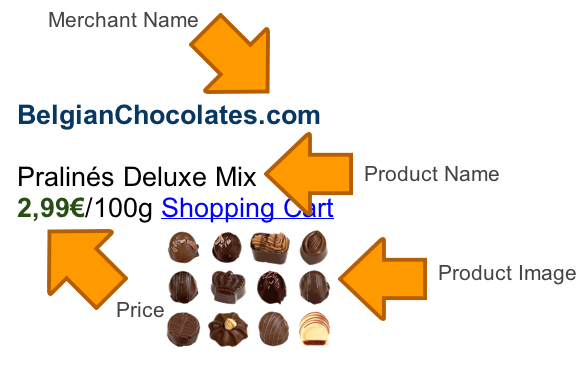
\includegraphics[width=0.468\textwidth]{fundamental-shift-2.png}
  }
  \caption{Fundamental shift from moving bits to moving bits with a~meaning}
  \label{fig:fundamental-shift}  
\end{figure}

\subsection{The Non-Semantic Web} \label{sec:non-semantic-web}

To differentiate the Semantic Web from the non-semantic Web,
it helps to step back one step and
see why the non-semantic Web is not semantic.
The Web is a~system of interlinked hypertext documents
accessed through the Internet.
These documents are typically marked up in
the Hypertext Markup Language (HTML),
a~language that defines a~syntax
understandable to user agents like Web browsers,
however, not one that provides meaning
beyond the level of text layout.
This means that an HTML snippet like
\begin{verbatim}
<h1>The Catcher in the Rye</h1>
<h2>J. D. Salinger</h2>
\end{verbatim}
reveals that \emph{The Catcher in the Rye}
is a~level one header element and
that \emph{J. D. Salinger} a~level two header element,
but to a~machine it is not evident that the prior
is the title of a~book,
and that the latter is (i) an author, and (ii)
the author of \emph{The Catcher in the Rye}.

\subsection{Structured Data on the Web}

A~very first step towards adding semantics to the Web
is using tabular data.
\autoref{tab:sample-table-structured-data} shows an example
for such tabular data.
For human beings (interested in sports),
the meaning of the columns in
\autoref{tab:sample-table-structured-data} is clear:

\begin{small_itemize}
  \item[] P = matches \textbf{P}layed
  \item[] W = \textbf{W}ins 
  \item[] D = \textbf{D}raws
  \item[] L = \textbf{L}osses
  \item[] F = Goals \textbf{F}or
  \item[] A = Goals \textbf{A}gainst
  \item[] Pts = \textbf{P}oin\textbf{ts}
\end{small_itemize}

\begin{table}[!ht]
\centering
    \begin{tabular}{l*{6}{c}r}
Team              & P & W & D & L & F  & A & Pts \\
\hline
Manchester United & 6 & 4 & 0 & 2 & 10 & 5 & 12  \\
Celtic            & 6 & 3 & 0 & 3 &  8 & 9 &  9  \\
Benfica           & 6 & 2 & 1 & 3 &  7 & 8 &  7  \\
FC Copenhagen     & 6 & 2 & 1 & 2 &  5 & 8 &  7  \\
    \end{tabular}
    \caption{Sample table with structured data for sports results}
    \label{tab:sample-table-structured-data}
\end{table}

The problem, however, is for machines to understand
the structure of the table.
Let us imagine one wanted to automate the task
of retrieving sports results from a~Web page with tabular data.
While it is a~straightforward job to implement
a~scraper bot that searches for column titles
like ``P'', ``W'', ``D'', \emph{etc.},
it would require the same work over and over again
for a~different language,
for example, German, where the terms would be:
``Sp.''~(Spiele), ``g.''~(gewonnen), ``u.''~(unentschieden),
``v.''~(verloren), ``Tore''~(Tore), ``Pkte.''~(Punkte).
A~German-speaking reader might have noticed
that the exemplary German system listed here
does not differentiate between \emph{goals for}
and \emph{goals against}, but only has a~list of \emph{Goals}.
Tiny differences like this make the scraping approach brittle.
If data providers were to use unique column identifiers like
Unique Resource Identifiers (URIs),
the problem would be easier.
In the concrete example for English and German,
rather than using ``D'' (\emph{Draws})
and ``u.'' (\emph{unentschieden}),
which both mean that the result was a~tie,
the machine-readable column name could instead be identified by
a~\emph{Unique} Resource Identifier (URI) like
\url{http://dbpedia.org/page/Tie_(draw)},
or even a~fictive URI like \url{http://example.org/VGllXyhkcmF3KQ==}.
In the next section, we therefore introduce
the structured knowledge base and interlinking hub
in the Web of Data, DBpedia~\cite{auer2007dbpedia}.

\subsection{The Structured Knowledge Base DBpedia}

An often reoccurring pattern
in the Semantic Web world
is the use of DBpedia~\cite{auer2007dbpedia}
as a~hub for identifying concepts by URIs.
DBpedia is a~Semantic Web knowledge base
with the objective of automatically extracting
pre-structured tabular data from the human-generated info-boxes
from the online encyclopedia
Wikipedia.\footnote{\url{http://en.wikipedia.org/wiki/Main_Page},
accessed July 15, 2013}
This pre-structured information is then made available
on the World Wide Web in many formats,
for example, in JSON~\cite{crockford2006json}
and many RDF~\cite{klyne2004rdf} serializations.
DBpedia allows for querying relationships
and properties associated with Wikipedia resources,
including links to other related datasets.
As outlined before, the concept of a~tie draw
in the sense of sports could thus be uniquely identified
by the DBpedia URI \url{http://dbpedia.org/page/Tie_(draw)},
free of all ambiguity.
Similar knowledge bases are among others
Freebase~\cite{markoff2007freebase},
YAGO~\cite{suchanek2007yago}, and CYC~\cite{lenat1995cyc}.

\subsection{Semantics in HTML Versions 4.01 and 5}

As outlined in \autoref{sec:non-semantic-web},
HTML versions 4.01~\cite{raggett1999html}
and 5~\cite{berjon2012html5}
contain a~basic level of semantics.
The main focus, however, is on the separation of
the markup of the textual structure from the actual presentation.
For example the \texttt{<b>} and the \texttt{<strong>} tags
both have the same visual effect:
they make the node value appear in a~bold face \textbf{like so}.
Visually, there is no way to differentiate between the two,
however, semantically the difference exists and is well-defined:
\texttt{<strong>} should be used when
one wants to give special emphasis on something.
Screen readers will typically read out such text
with a~more emphasized voice.
In contrast, \texttt{<b>} should be used
if only visually one wants to create a~bold face look.
In the following, we present a~list of semantic HTML tags
and attributes and their meaning.

\paragraph{Semantic HTML 4.01 Tags:}

\begin{itemize}
  \item \texttt{<abbr>} specifies an abbreviation,
        \texttt{<acronym>} specifies an acronym.
  \item \texttt{<h1>--<h6>} specify level 1--6 headers,
        \texttt{<caption>} specifies a~caption for a~table.
  \item \texttt{<blockquote>} specifies a~block-level quotation
        (a~source in form of a~URI may be specified via the
        \texttt{cite} attribute),
        \texttt{<cite>} specifies a~citation.
  \item \texttt{<dl>} specifies a~definition list, \texttt{<dt>}
        specifies a~definition term in a~definition list,
        \texttt{<dd>} specifies the definition of a~term
        in a~definition list.
  \item \texttt{<em>} specifies an emphasis, \texttt{<strong>}
        specifies a~strong emphasis.
  \item \texttt{<code>} specifies a~code snippet, \texttt{<dfn>}
        specifies an inline definition of a~single term,
        \texttt{<address>} specifies contact information
        for the document author, \texttt{<legend>} specifies
        a~legend for \texttt{<fieldset>} containers
        for adding structure to forms,
        \texttt{<samp>} specifies sample output
        from a~script or program.
\end{itemize}

\paragraph{Semantic HTML5 Tags:}

\begin{itemize}
  \item \texttt{<article>} specifies an independent item
        section of content,
        \texttt{<aside>} specifies a~section of a~page that
        consists of content that is tangentially related
        to the content around the \texttt{<aside>} element,
        and which could be considered separate from
        that content, \texttt{<header>} specifies a~group of
        introductory or navigational aids,
        \texttt{<footer>} specifies a~footer for its nearest
        ancestor sectioning content or sectioning root element,
        \texttt{<nav>} specifies a~section with navigation links.
  \item \texttt{<figure>} specifies some flow content,
        \texttt{<mark>} specifies a~run of text in one document
        marked or highlighted for reference purposes
        due to its relevance in another context,
        \texttt{<meter>} specifies a~scalar measurement within
        a~known range, or a~fractional value.
  \item \texttt{<audio>} specifies a~sound or an audio stream,
        \texttt{<video>} specifies a~video or movie.
  \item \texttt{<progress>} specifies the completion progress
        of a~task, \texttt{<time>} specifies either a~time
        on a~24 hour clock, or a~precise date in the calendar
        (optionally with a~time and a~time-zone offset),
        \texttt{<command>} specifies a~command that the user
        can invoke.
  \item \texttt{<details>} specifies a~disclosure widget
        from which the user can obtain additional information or
        controls, \texttt{<datalist>} specifies the list that
        represents predefined options for input elements.
  \item \texttt{<keygen>} specifies a~key pair generator control,
        \texttt{<output>} specifies the result of a~calculation,
        \texttt{<ruby>} allows one or more spans of phrasing
        content to be marked with ruby annotations.
\end{itemize}

\paragraph{HTML5 Input Type Attributes:}

\begin{itemize}
  \item \texttt{datetime} specifies a~control for setting the
        element’s value to a~string representing a~global date
        and time (with timezone information).
  \item \texttt{datetime-local} specifies a~control for setting
        the element’s value to a~string representing a~local date
        and time (with no timezone information).
  \item \texttt{date} specifies a~control for setting the 
        element’s value to a~string representing a~date,
        \texttt{month} specifies a~control for setting the
        element’s value to a~string representing a~month,
        \texttt{week} specifies a~control for setting the
        element’s value to a~string representing a~week.
  \item \texttt{time} specifies a~control for setting the
        element’s value to a~string representing a~time
        (with no timezone information).
  \item \texttt{number} specifies a~control for setting the
        element’s value to a~string representing a~number.
  \item \texttt{range} represents an imprecise control
        for setting the element’s value to a~string
        representing a~number.
  \item \texttt{email} specifies a~control for editing
        a~list of email addresses given in the element’s value.
  \item \texttt{url} specifies a~control for editing an
        absolute URL given in the element’s value.
  \item \texttt{search} specifies a~one-line plain-text
        edit control for entering one or more search terms.
  \item \texttt{color} specifies a~color-well control for
        setting the element’s value to a~string representing
        a~simple color.
\end{itemize}

\subsection{Structured Data Beyond Pure HTML}

In this subsection, we describe how structured data
can be included in HTML documents
by either overloading existing HTML attributes
or by adding new ones.

\subsubsection{Microformats}

Microformats~\cite{celik2006microformats} are a~set of
open data mark-up formats developed
and defined by the Microformats
community.\footnote{\url{http://microformats.org/discuss},
accessed July 15, 2013}
Microformats are not an official standard,
but rather a~widely adopted grass-roots-driven movement
with origins in the blogging scene.
It is to be noted that Microformats do not require a~new language,
but reuse building blocks from widely adopted standards
such as the \texttt{class}, \texttt{rel}, and \texttt{title}
attributes in HTML.
Their main design goal is to focus first on humans,
then on machines.
A~concrete example of Microformat mark-up in HTML
can be seen in \autoref{code:microformats}.
There are currently nine stable
Microformats,\footnote{\url{http://microformats.org/wiki/Main_Page\#Specifications}, accessed July 15, 2013}
as listed below:

\begin{itemize}
  \item \texttt{hCalendar} is a~distributed calendaring and
        events format, using a~1:1 representation of the standard
        \texttt{iCalendar} format
        (RFC~2445,~\cite{dawson1998icalendar}).
  \item \texttt{hCard} is a~format for representing people,
        companies, organizations, and places, using a~1:1
        representation of the standard \texttt{vCard} format
        (RFC~2426,~\cite{dawson1998vcard}).
  \item \texttt{rel-license} is a~format for indicating content
        licenses, which is embeddable in
        HTML~\cite{raggett1999html} or
        XHTML~\cite{pemberton2000xhtml},
        Atom~\cite{nottingham2005atom},
        RSS~\cite{cadenhead2006rss},
        and arbitrary XML~\cite{bray2008xml}.
  \item \texttt{rel-nofollow} is a~format for hyperlinks
        indicating that the destination of that hyperlink should
        not be afforded any additional weight or ranking by user
        agents such as search engines, which perform link
        analysis upon Web pages.
  \item \texttt{rel-tag} is a~format for hyperlinks indicating
        that the destination of that hyperlink is an
        author-designated keyword for the current page.
  \item \texttt{VoteLinks} is a~format for adding the idea of
        agreement, abstention or indifference, and disagreement
        to hyperlinks.
  \item \texttt{XFN} is a~format for representing human
        relationships using hyperlinks, which enables Web authors
        to indicate their relationships to people.
  \item \texttt{XMDP} is a~format for defining metadata profile
        documents (XHTML Meta Data Profile), which enables Web
        authors to well-define custom meta tags.
  \item \texttt{XOXO} is a~format for defining a~new
        XHTML~\cite{pemberton2000xhtml}
        document type for subsetting and extending XHTML,
        which serves as the basis for XHTML-friendly outlines for
        processing by XML engines, and for easy interactive
        rendering by browsers.
\end{itemize}

\begin{lstlisting}[caption={
   [Sample code snippet with embedded hCard Microformat mark-up]
   {Sample code snippet with embedded \texttt{hCard} Microformat
    mark-up (\url{http://microformats.org/wiki/hcard})}
  },
  label={code:microformats}]
<div class="vcard">
  <a class="fn org url" href="http://www.commerce.net/">CommerceNet</a>
  <div class="adr">
    <span class="type">Work</span>:
    <div class="street-address">169 University Avenue</div>
    <span class="locality">Palo Alto</span>,  
    <abbr class="region" title="California">CA</abbr>&nbsp;&nbsp;
    <span class="postal-code">94301</span>
    <div class="country-name">USA</div>
  </div>
  <div class="tel">
   <span class="type">Work</span> +1-650-289-4040
  </div>
  <div class="tel">
    <span class="type">Fax</span> +1-650-289-4041
  </div>
  <div>Email: 
   <span class="email">info@commerce.net</span>
  </div>
</div>
\end{lstlisting}

\subsubsection{Microdata}

Microdata~\cite{hickson2012microdata} defines a~way to annotate 
content (or items) with specific machine-readable labels,
for example, to allow scripts to provide services that are
customized to a~website.
Microdata allows for nested groups of name-value pairs
to be added to documents,
in parallel with the existing content.
The Microdata specification introduces
a~set of new attributes to HTML:

\begin{itemize}
  \item \texttt{itemscope} creates an item (or thing) and
        indicates that descendants of this element contain
        information about it. This attribute precedes the
        \texttt{itemtype} attribute in the HTML element's tag.
  \item \texttt{itemtype} a~valid URL of a~vocabulary that
        describes the item and its properties context.
  \item \texttt{itemid} indicates a~unique identifier
        of the item in the vocabulary.
  \item \texttt{itemprop} indicates that its containing tag
        holds the value of the specified item property.
        The properties name and value context are described by
        the items vocabulary. Properties values usually
        consist of string values,
        but can also use URLs using the \texttt{<a>} tag
        and its \texttt{href} attribute,
        the \texttt{<img>} tag and its \texttt{src} attribute,
        or other tags that link to or embed external resources.
  \item \texttt{itemref} properties that are not descendants of
        the element with the \texttt{itemscope} attribute
        can be associated with the item using this attribute.
        It provides a~list of elements to Web crawlers to find
        additional property values of the item
        elsewhere in the document.
\end{itemize}

An example of Microdata in HTML can be seen in \autoref{code:microdata}.

\begin{lstlisting}[caption={
  [Sample code snippet with Microdata mark-up]
  {Sample code snippet with Microdata mark-up
   (\url{http://www.w3.org/TR/microdata/})}},
  label={code:microdata}]
<div itemscope>
  <p>My name is <span itemprop="name">Neil</span>.</p>
  <p>
    My band is called
    <span itemprop="band">Four Parts Water</span>.
  </p>
  <p>I am <span itemprop="nationality">British</span>.</p>
</div>
\end{lstlisting}

\section{Resource Description Framework (RDF)} \label{sec:rdf}

The Resource Description Framework (RDF,~\cite{klyne2004rdf})
defines a~set of W3C standards for the formal description of
resources that are identified by URIs.
RDF is a~core component of the Semantic Web.
Initially, it was designed to describe metadata
on the World Wide Web (WWW) such as authors,
copyrights, \emph{etc.}\ of documents, however,
applying a~definition of the term \emph{resource}
beyond the WWW context,
RDF is now also used to describe metadata
of any URI-identifiable entity like cities, genes, \emph{etc.}

\subsection{Triples as a~Data Structure}

As outlined before, one of the main purposes of the Semantic Web
is to give information a~well-defined meaning.
Using an example from Tim Berners-Lee’s
article~\cite{bernerslee2001semanticweb},
meaning can be to differentiate between the concepts of
a~shipping and a~billing address,
or the concept of an address in the sense of
delivering a~formal spoken communication to an audience.
In order to assure the differences in meaning,
things are identified by a~Unique Resource Identifier (URI).
The majority of the data processed by machines
can be described by elementary sentences like
\emph{A~cat is a~mammal},
\emph{Thomas Steiner is the author of this document},
or \emph{Prince William is married to Kate Middleton}.
Each of these sentences has a~subject (\emph{A~cat}),
a~predicate (\emph{is a}), and an object (\emph{mammal}).
Every subject, predicate, and object can be identified by a~URI.
This idea is very powerful,
as it allows to express the same concept
represented by a~URI (for example, mammal by
\url{http://dbpedia.org/resource/Mammal})
with different terms in different languages
(like, for example, Säugetier, mammal, or nisäkkäät).
Everyone can extend the set of concepts
simply by creating a~URI on the Web.
This form of knowledge representation
is used by the Resource Description Framework.

\subsection{Important RDF Serialization Syntaxes}

Knowledge or facts represented in the RDF triple data structure
need to be serialized in order to be stored
or transmitted over the Internet.
Several serialization formats exist,
each of which with its particular advantages
and disadvantages, mostly around readability for human beings
and parsability for machines.
According to our experience, most people prefer the Turtle~\cite{prudhommeaux2013turtle}
format for its readability,
whereas for machines, oftentimes RDF/XML~\cite{beckett2004rdfxml}
is the easiest to work with.

\subsubsection{RDF Sample Graph}
In the following, we will illustrate the various
RDF serialization formats with an RDF sample graph
inspired by a~default example of the Apache Anything To Triples project
(Any23,~\url{http://any23.org/}, accessed July 15, 2013).
It contains data about a~fictive FOAF~\cite{brickley2010foaf}
person named \emph{John X. Foobar}
with an email address with the SHA1 checksum of
\emph{cef817456278b70cee8e5a1611539\-ef9d928810e}.
The actual email address is obscured to avoid spam emails.
\autoref{fig:sample-rdf-graph} shows the graphical representation
of this sample graph.

\begin{figure}[!ht]
\centering
  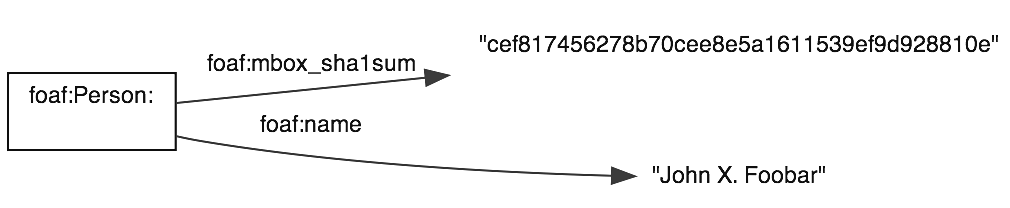
\includegraphics[width=\linewidth]{sample-rdf-graph.png} 
  \caption{Sample RDF graph visualized}
  \label{fig:sample-rdf-graph}
\end{figure}

\subsubsection{The RDF/XML Syntax}

RDF/XML~\cite{beckett2004rdfxml} was introduced by
the W3C as the first RDF serialization syntax.
Albeit more human-friendly serialization formats
such as Turtle~\cite{prudhommeaux2013turtle}
gain more and more traction,
RDF/XML is still very wide-spread.
Its media type is \texttt{application/rdf+xml},
the recommended file extension is \texttt{.rdf},
the encoding is UTF-8.
\autoref{code:rdfxml-syntax} shows the previously
introduced sample graph serialized in RDF/XML.

\begin{lstlisting}[caption={Sample graph in RDF/XML syntax},
  label={code:rdfxml-syntax}]
<?xml version="1.0" encoding="UTF-8"?>
<rdf:RDF
    xmlns:foaf="http://xmlns.com/foaf/0.1/"
    xmlns:rdf="http://www.w3.org/1999/02/22-rdf-syntax-ns#">
  <rdf:Description rdf:nodeID="node15urahancx74224">
    <rdf:type rdf:resource="http://xmlns.com/foaf/0.1/Person"/>
    <foaf:name>John X. Foobar</foaf:name>
    <foaf:mbox_sha1sum>
      cef817456278b70cee8e5a1611539ef9d928810e
    </foaf:mbox_sha1sum>
  </rdf:Description>
</rdf:RDF>
\end{lstlisting}

\subsubsection{The N-Triples Syntax} \label{sec:n-triples}

The N-Triples~\cite{grant2004ntriples} syntax was primarily
developed by Dave Beckett and Art Barstow.
N-Triples is a~subset of Turtle (see \autoref{sec:turtle}),
which in turn is a~subset of Notation3
(see \autoref{sec:notation3}).
There are very few variations to express a~graph in N-Triples,
which makes it an ideal syntax for testing purposes, however,
as it is missing some shortcuts of Turtle, it is quite verbose.
Its media type is \texttt{text/plain}, the recommended file extension is \texttt{.nt},
and the encoding is 7-bit US-ASCII
(and explicitly \emph{not} UTF-8).
\autoref{code:ntriples-syntax} shows the previously
introduced sample graph serialized in N-Triples.

\begin{lstlisting}[caption={Sample graph in N-Triples syntax},
  label={code:ntriples-syntax}]
_:1 <http://www.w3.org/1999/02/22-rdf-syntax-ns#type>
    <http://xmlns.com/foaf/0.1/Person> .
_:1 <http://xmlns.com/foaf/0.1/name>
    "John X. Foobar" .
_:1 <http://xmlns.com/foaf/0.1/mbox_sha1sum>
    "cef817456278b70cee8e5a1611539ef9d928810e" .
\end{lstlisting}

\subsubsection{The Turtle Syntax} \label{sec:turtle}

Turtle~\cite{prudhommeaux2013turtle},
or the Terse RDF Triple Language, was defined by Dave Beckett.
It is a~superset of N-Triples (see \autoref{sec:n-triples}) and
a~subset of Notation3 (see \autoref{sec:notation3}).
It has reached a~\emph{de~facto} standard status,
with the RDF Working Group publishing the new Turtle specification
as a~W3C Candidate Recommendation on February 19, 2013.
Its media type is \texttt{text/turtle}
(the sometimes still observable media type
\texttt{application/x-turtle} is deprecated),
the recommended file extension is \texttt{.ttl},
the encoding is UTF-8.
\autoref{code:turtle-syntax} shows the previously
introduced sample graph serialized in Turtle.

\begin{lstlisting}[caption={[Sample graph in Turtle syntax]{Sample graph in Turtle syntax,
  the syntax is equivalent to \autoref{code:notation3-syntax}}},
  label={code:turtle-syntax}]
@prefix foaf: <http://xmlns.com/foaf/0.1/> .

_:node15urahancx74223 a foaf:Person ;
  foaf:name "John X. Foobar" ;
  foaf:mbox_sha1sum "cef817456278b70cee8e5a1611539ef9d928810e" .
\end{lstlisting}

\subsubsection{The Notation3 Syntax} \label{sec:notation3}

Notation3~\cite{bernerslee2011notation3} was introduced
by Tim Berners-Lee.
Notation3 has some features that go beyond
the pure expressiveness of RDF like rules,
support for variables, and quantification.
Its media type is \texttt{text/n3},
the recommended file extension is \texttt{.n3},
the encoding is always UTF-8.
\autoref{code:notation3-syntax} shows the previously
introduced sample graph serialized in Notation3,
which, given the present trivial example,
is syntactically equal to Turtle.

\begin{lstlisting}[caption={Sample graph in Notation3 syntax},
  label={code:notation3-syntax}]
@prefix foaf: <http://xmlns.com/foaf/0.1/> .

_:node15urahancx74223 a foaf:Person ;
  foaf:name "John X. Foobar" ;
  foaf:mbox_sha1sum "cef817456278b70cee8e5a1611539ef9d928810e" .
\end{lstlisting}

\subsubsection{The RDFa Syntax}

RDFa~\cite{adida2012rdfa} has a~special role
in that it is a~specification for attributes
to express structured data in XHTML~\cite{pemberton2000xhtml},
but also in HTML4 and HTML5~\cite{sporny2012htmlrdfa}.
It uses the rendered hypertext content of (X)HTML
for the RDFa markup,
so that data publishers can use the same document
for human- and machine-readable content.
The contained RDF triples can be extracted with distillers.
In consequence, RDFa can be considered
another serialization syntax for RDF,
with the same expressive power as
RDF/XML~\cite{beckett2004rdfxml},
Turtle~\cite{prudhommeaux2013turtle}, \emph{etc.}
Its media type is \texttt{application/xhtml+xml},
the recommended file extension is \texttt{.html}.
RDFa shares some design goals
with Microformats~\cite{celik2006microformats}
and Microdata~\cite{hickson2012microdata}.
Where Microformats specify both a~syntax
for embedding structured data into HTML
\emph{and} a~vocabulary of specific terms for each Microformat,
RDFa in contrast \emph{only} specifies a~syntax,
since the vocabularies it relies on
are externally and independently specified.
The essence of RDFa is a~set of attributes
that contain metadata about things,
and that can be embedded in mark-up languages,
for example in XHTML or HTML.
The concrete attributes are as follows.

\begin{itemize}
  \item \texttt{about} and \texttt{src} a~URI or
        CURIE (compact URI)~\cite{birbeck2007curie}
        that specifies the resource
        the metadata is about.
  \item \texttt{rel} specifies a~relationship with
        another resource.
  \item \texttt{href} and \texttt{resource} specify
        the partner resource.
  \item \texttt{property} specifies a~property for
        the content of an element.
  \item \texttt{content} optional attribute that overrides
        the content of the element when using
        the property attribute.
  \item \texttt{datatype} optional attribute that
        specifies the datatype of text specified
        for use with the property attribute.
  \item \texttt{typeof} optional attribute that specifies
        the RDF type(s) of the subject (the resource
        that the metadata is about).
\end{itemize}

An additional simplified subset of RDFa is RDFa Lite~\cite{sporny2012rdfaalite}, which is aligned with Microdata.
\autoref{code:rdfa-syntax} shows the previously introduced
sample graph serialized in RDFa.

\begin{lstlisting}[caption={Sample graph in RDFa syntax},
  label={code:rdfa-syntax}]
<div about="_:1" typeof="http://xmlns.com/foaf/0.1/Person">           
  <span property="http://xmlns.com/foaf/0.1/mbox_sha1sum">
    cef817456278b70cee8e5a1611539ef9d928810e
  </span> 
  <span property="http://xmlns.com/foaf/0.1/name">
    John X. Foobar
  </span>
</div> 
\end{lstlisting}

\section{SPARQL: Semantic Web Query Language}

SPARQL is a~recursive acronym that stands for
SPARQL Protocol and RDF Query Language.
The SPARQL specification~\cite{prudhommeaux2008sparql}
defines the syntax and semantics
of the SPARQL query language for RDF.
RDF~\cite{klyne2004rdf} is a~directed, labeled
graph data format for representing information on the Web.
SPARQL can be used to express queries
across diverse data sources,
whether the data is stored natively as RDF,
or viewed as RDF via middleware.
SPARQL allows for querying required
and optional graph patterns
along with their conjunctions and disjunctions.
SPARQL also supports extensible value testing
and constraining queries by source RDF graph.
The results of SPARQL queries can be result sets or RDF graphs.
SPARQL became an official W3C Recommendation in 2008.
It was standardized by the RDF Data Access Working Group (DAWG).

\subsection{The Vision of the Web as a~Giant Single Database}

The Web as we know it today is a~\emph{network of documents},
interconnected by hyperlinks that everyone can participate in
by placing links to existing documents.
The vision of the Semantic Web, however,
is a~\emph{network of facts} about entities,
interconnected by means of graphs of data.
Where the Web of today is a~graph of documents,
the Semantic Web is envisioned to be a~huge global graph,
formed by many individual graphs.
If one party publishes facts about an entity
and a~different party publishes different facts
about the same entity,
then the overall knowledge about that entity
is represented in a~decentralized way,
accessible to all, and open for everyone to enrich.
This requires strong globally unique identifiers,
or at least ways to map one identifier to another.

Given the (visionary) huge global graph, a~fictive
SPARQL query like the one in \autoref{code:sparql}
could be used to get results from the graph,
like the email addresses of every person in the world.
SPARQL queries, unlike traditional databases, are not necessarily
guaranteed to return \emph{all} existing results (completeness).

\begin{lstlisting}[caption={[Fictive SPARQL query returning names and
  email addresses]
  {Fictive SPARQL query returning the names and email addresses of every
  person in the world
  (\url{http://en.wikipedia.org/wiki/SPARQL\#Benefits}, accessed July 15, 2013)}},
  label={code:sparql}]
PREFIX foaf: <http://xmlns.com/foaf/0.1/>
SELECT ?name ?email
WHERE {
  ?person a foaf:Person.
  ?person foaf:name ?name.
  ?person foaf:mbox ?email.
}
\end{lstlisting}

This query selects the names and email addresses from all persons
who have facts about them in the global graph.
The query starts with a~prefix definition,
and then constrains the results
to be of type \texttt{foaf:Person}~\cite{brickley2010foaf},
whose name and email address are the values
of the triples with the predicates \texttt{foaf:name}
and \texttt{foaf:mbox} respectively.
While this sounds like a~very powerful idea,
in practice SPARQL endpoints
like the DBpedia SPARQL
endpoint\footnote{\url{http://dbpedia.org/sparql}, accessed July 15, 2013}
typically only allow for querying a~local graph
for performance reasons.

\subsection{Different SPARQL Query Variations}

The SPARQL Query Language currently specifies four different query variants, which we will list in the following. 

\subsubsection{SELECT}

The \texttt{SELECT} query variant is used to extract
raw values from a~SPARQL endpoint.
The results are returned in a~tabular format.
A~sample query was given in \autoref{code:sparql}.

\subsubsection{DESCRIBE}

The \texttt{DESCRIBE} query variant is used to extract
an RDF graph from the SPARQL endpoint,
the contents of which is left to the endpoint to decide
based on what the maintainer deems as useful information.
An example query is given below:\\

\texttt{DESCRIBE <http://example.org/sparql>}

\subsubsection{ASK}

The \texttt{ASK} query variant is used to provide
a~simple \texttt{true} or \texttt{false} result
for a~query on a~SPARQL endpoint.
No information is returned about the possible query solutions,
just whether or not a~solution exists.
An example query with a~sample response is given below:\\

\noindent Given the RDF graph in \autoref{fig:sample-rdf-graph}
and the following SPARQL \texttt{ASK} query:\\

\texttt{PREFIX foaf: <http://xmlns.com/foaf/0.1/>\\
\indent ASK \{ ?x foaf:name  "Alice" \}}\\

\noindent This query creates the following response
(as there is no person named Alice in the graph,
but only a~person named John X. Foobar):\\

\texttt{no}

\subsubsection{CONSTRUCT}

The \texttt{CONSTRUCT} query variant is used to extract
information from the SPARQL endpoint
and to transform the results into valid RDF
specified by a~graph template.
The result is an RDF graph formed by taking
each query solution in the solution sequence,
substituting for the variables in the graph template,
and combining the resulting triples into
a~single RDF graph by set union.
An example query is given below.\\

\noindent Given the following RDF graph,
serialized in Turtle syntax:\\

\texttt{@prefix foaf: <http://xmlns.com/foaf/0.1/> .}\\
\texttt{\indent \_:a foaf:name "Alice" .}\\
\texttt{\indent \_:a foaf:mbox <mailto:alice@example.org> .}\\

\noindent Given the following SPARQL \texttt{CONSTRUCT} query:\\

\texttt{PREFIX foaf: <http://xmlns.com/foaf/0.1/>}\\
\texttt{\indent PREFIX vcard: <http://www.w3.org/2001/vcard-rdf/3.0\#>}\\
\texttt{\indent CONSTRUCT \{ <http://example.org/person\#Alice> vcard:FN ?name \}}\\
\texttt{\indent WHERE { ?x foaf:name ?name }}\\

\noindent This query creates the following
\texttt{vcard}~\cite{dawson1998vcard}
properties from the FOAF information:\\

\texttt{@prefix vcard: <http://www.w3.org/2001/vcard-rdf/3.0\#> .}\\ 
\texttt{\indent <http://example.org/person\#Alice> vcard:FN "Alice" .}

\section{Linked Data}

Linked Data~\cite{bernerslee2006linkeddata}
defines a~set of agreed-on best practices and
principles for interconnecting and publishing
structured data on the Web.
It uses Web technologies like HTTP~\cite{fielding1999http}
and URIs~\cite{bernerslee2005uri}
to create typed links between different sources.
The portal \url{http://linkeddata.org/} (accessed July 15, 2013)
defines Linked Data as being
\textit{``about using the Web to connect related data that
wasn’t previously linked, or using the Web
to lower the barriers to linking data
currently linked using other methods''}.

\subsection{The Linked Data Principles}
\label{sec:linked-data-principles}

Tim Berners-Lee defines the four rules for Linked Data in a~W3C Design Issue~\cite{bernerslee2006linkeddata} as follows:

\begin{enumerate}
  \item Use URIs as names for things.
  \item Use HTTP URIs so that people can look up those names.
  \item When someone looks up a~URI, provide useful information,
        using the standards (RDF*, SPARQL).
  \item Include links to other URIs,
        so that they can discover more things.
\end{enumerate}

Linked Data uses RDF~\cite{klyne2004rdf} to create
typed links between things in the world.
The result is oftentimes referred to as the \emph{Web of Data}.
As outlined before, RDF encodes statements
about things in the form of
\texttt{(subject, predicate, object)} triples.
If subject and object have URIs from different namespaces,
Bizer \emph{et~al.}\ speak of \emph{RDF links}
in~\cite{heath2011linkeddata}.
An exemplary RDF link adapted from~\cite{bizer2009linkeddatastory}
stating that a~description of the movie Pulp Fiction
from the Linked Movie Database~\cite{hassanzadeh2009linkedmovie}
and a~description from DBpedia~\cite{auer2007dbpedia}
are indeed talking about the same movie
can be seen in \autoref{code:rdflink}.

\begin{lstlisting}[caption={[Exemplary RDF link]{Exemplary RDF
  link stating that a~description of the movie Pulp Fiction from
  the Linked Movie Database~\cite{hassanzadeh2009linkedmovie}
  and a~description from DBpedia are indeed talking
  about the same movie}},
  label={code:rdflink},
  escapechar=§]
<http://data.linkedmdb.org/resource/film/77> §\linewrap§
  <http://www.w3.org/2002/07/owl#sameAs> §\linewrap§
  <http://dbpedia.org/page/Pulp_Fiction> .
\end{lstlisting}

\subsection{The Linking Open Data Cloud Diagram}
\label{sec:lodcloud}

The Linking Open Data (LOD) cloud
diagram~\cite{cyganiak2011lodcloud} is a~visualization effort
that shows datasets that have been published in
Linked Data~\cite{bernerslee2006linkeddata}
format by contributors to the Linking Open Data community project
and other individuals and organizations.
The objective is to identify existing datasets with open licenses,
convert them to RDF whilst obeying the Linked Data principles,
and finally publish them on the Web.
Due to its open structure, everyone can contribute to the project by publishing a~dataset and
interlinking it to existing datasets.
Today, the project includes datasets of major organizations
such as the BBC, Thomson Reuters, or the Library of Congress
to name just a~few.
The state of the LOD cloud has been examined
in~\cite{bizer2011statelodcloud}.
The latest LOD cloud diagram as of September 2011 can be seen in \autoref{fig:lod-cloud}.

\begin{figure}[!ht]
\centering  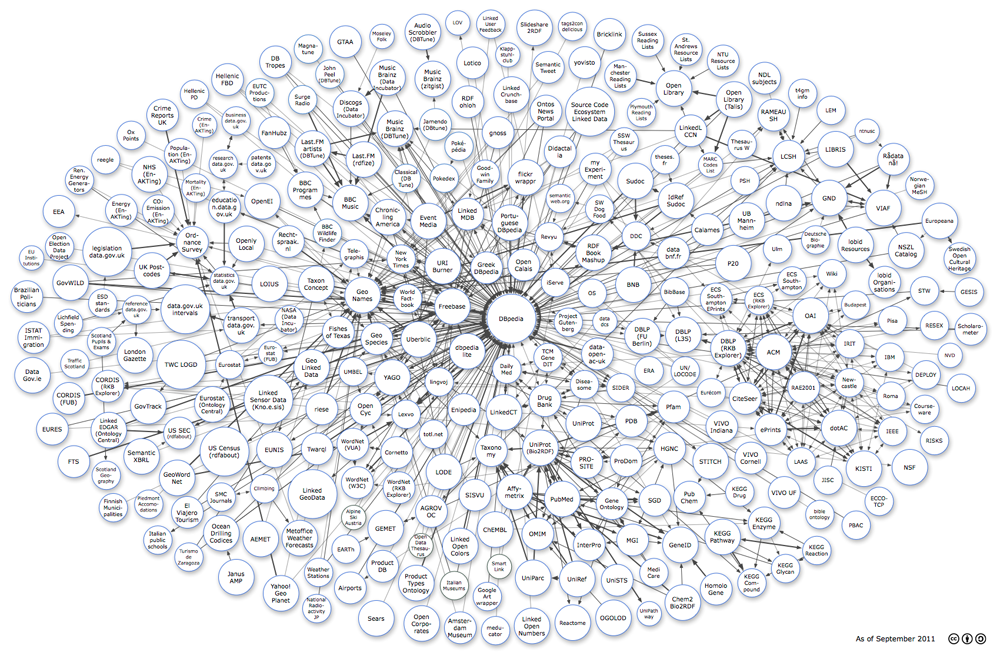
\includegraphics[height=0.8\textheight,keepaspectratio]{lod-cloud.png}    
  \caption[Linking Open Data cloud diagram as of September 2011]
  {Linking Open Data cloud diagram as of September 2011, by Richard Cyganiak and Anja Jentzsch \url{http://lod-cloud.net/} (accessed July 15, 2013) \todo{Check final orientation}}    
  \label{fig:lod-cloud}
\end{figure}

\section{Conclusions}

In this chapter, we have first introduced the Semantic Web
and compared it to the non-semantic Web.
We have shown how structured data in the form of tables
is a~first step towards richer semantics.
An example of converting structured data from Wikipedia
into machine-readable data is the knowledge base DBpedia.
Further, we have looked at the intrinsic semantics
of HTML in versions 4 and 5,
and how through additional attributes
even richer semantics can be added
by the annotation formats Microdata and Microformats.
We have introduced the Resource Description Format (RDF)
and its different serializations.
On top of RDF, we have detailed
how the Semantic Web query language SPARQL
can be used to express queries across data sources.
Finally, we have shown how data on the Web
can be exposed as so-called Linked Data,
an effort which is visualized in the Linking Open Data cloud.
By introducing these Semantic Web technologies,
we have set the foundations for the coming chapters
that build upon those pillars.

\section*{Chapter Notes}
This chapter is partly based on the following publications:
\todo{Add publications}

\bibliographystyle{plainnat}
\clearpage
\bibliography{backmatter/references}

\chapter{Social Networks}
\label{cha:social-networks}

% the code below specifies where the figures are stored
\ifpdf
    \graphicspath{{3_social_networks/figures/PNG/}{3_social_networks/figures/PDF/}{3_social_networks/figures/}}
\else
    \graphicspath{{3_social_networks/figures/EPS/}{3_social_networks/figures/}}
\fi

From the first ever email to video calls on the go,
the Internet has always been about communication.
Historically, communities formed around Usenet mailing lists or Bulletin Board Systems, starting from the early eighties,
often around all sorts of topics like fine arts,
literature, and philosophy (\emph{e.g.}, \texttt{humanities.classics}
or \texttt{humanities.\-design.misc}).
Then, starting from the late eighties, Internet Relay Chats (IRC)
allowed people to communicate interactively and in real-time,
organized in channels (\emph{e.g.}, \texttt{\#linux}).
Starting from the nineties, blogs began to spread,
reaching mainstream popularity somewhere in mid-2000.
While the early social communities
where created entirely \emph{ad-hoc}
whenever someone logged in to a~system,
the first social networks,
among them \url{http://sixdegrees.com/} in 1997,
allowed people to maintain a~public profile
with a~list of connections (\emph{friends})
that others could browse.
In~\cite{boyd2007socialnetworksites}, boyd
(\emph{sic}\footnote{http://www.danah.org/name.html})
and Ellison define the term
\emph{social network site (SNS)} as follows.

\begin{quotation}
  \textit{``We define social network sites as web-based services
  that allow individuals to
  (1) construct a~public or
  semi-public profile within a~bounded system,
  (2) articulate a~list of other users
  with whom they share a~connection, and
  (3) view and traverse their list of connections
  and those made by others within the system.
  The nature and nomenclature of these connections
  may vary from site to site.''}
\end{quotation}

Literature on social networks oftentimes uses the term SNS,
however, in order to differentiate ourselves
from the therein defined idea of social network,
we decided to avoid the term altogether in favor of a~more open
definition of social network,
which we detail in the following. 

\section{Definition of Terms Used in this Thesis}
\label{sec:definition}

In this section, we define the terms
that we will use throughout this thesis
in order to avoid any ambiguity.
In particular, we highlight that social networks have
different levels of support for media items.

\begin{description}
  \item[Social Network:]
       A~social network is an online service or media platform
       that focuses on building and reflecting
       relationships among people
       who share interests and/or activities.
  \item[Media Item:]
       A~media item is defined as
       a~photo\footnote{We chose the term \emph{photo}
       over the term \emph{image} as 
       Facebook, Twitter, and \googleplus use it.}
       or video
       file that gets distributed via a~social network.
  \item[Micropost:]
       A~micropost is defined as a~textual status message
       that can optionally be accompanied by a~media item.
  \item[Hashtag] The \texttt{\#} symbol, called a~hashtag,
       is used to mark keywords or topics in a~micropost.
       It was created organically by Twitter users
       as a~way to categorize messages.
       People use the hashtag symbol \texttt{\#} before a~relevant keyword
       or phrase (no spaces) in microposts to categorize them
       and help them show more easily in
       search\footnote{Adapted from
       \url{https://support.twitter.com/articles/49309-what-are-hashtags-symbols},
       accessed December 7, 2012.}. 
\end{description}

The boundary between \emph{social networks} and
\emph{media platforms} is blurred.
Several media sharing platforms, \emph{e.g.},
YouTube\footnote{http://youtube.com/},
enable people to upload content
and optionally allow other people to react
to this content in the form of comments, likes or dislikes.
On other social networks, \emph{e.g.},
Facebook\footnote{http://facebook.com/},
users can update their status, post links to stories,
upload media content, and also give readers the option to react.
Finally, there are hybrid clients, \emph{e.g.},
TweetDeck\footnote{http://www.tweetdeck.com/}
by Twitter together with
Twitpic\footnote{http://twitpic.com/},
where social networks integrate with media platforms,
typically via third-party applications.

\section{Description of Popular Social Networks}
\label{sec:description-of-popular-social-networks}

In this section, we introduce several social networks
and some of their key features
that are relevant for our approach.
As we treat all networks the same---%
independent from their not always publicly known user population---%
they are listed in alphabetic order.
For active participation,
all social networks require users to be logged in.
In the description below, we thus assume a~logged in user.

\subsection{Facebook}

Facebook (\url{http://www.facebook.com/})
is a~social networking service launched in February 2004,
operated and owned by the American multinational
Internet corporation Facebook, Inc.
At time of writing, Facebook is the most popular social network
with one billion monthly active
users\footnote{\url{http://newsroom.fb.com/Key-Facts},
accessed November 19, 2012}
as of October 2012.
Facebook has native photo and video support,
allowing people to upload an unlimited amount of media items.
Photos and videos can also be recorded \emph{ad hoc} via webcam.
People can \emph{Like} content via a~designated Like button
that can also be embedded on other websites.
Initially, the button was called the \emph{Awesome} button,
but eventually\footnote{\url{http://www.quora.com/Facebook-Inc-company/Whats-the-history-of-the-Awesome-Button-that-eventually-became-the-Like-button-on-Facebook}}
got rebranded to its current form.
Individual microposts can also be shared.
Facebook has a~bidirectional relationship model (friend model),
with an optional unidirectional relationship model (follow model),
typically for following celebrities, remote friends, \emph{etc.}

\subsection{Flickr}

Flickr (\url{http://www.flickr.com/})
is a~photo and video hosting online community
created by Ludicorp in 2004 and acquired by Yahoo! in 2005.
Users can upload a~limited or unlimited number of photos or videos
to the service, depending on their account type (Free or Pro).
People can \emph{Favorite} photos they like
via a~designated Favorite button.
Flickr has a~unidirectional relationship model (follow model),
however, also allows people to mark other users as friends
or family \emph{without} the other party having to confirm.
Following an urgent plea from Flickr
users\footnote{\url{http://dearmarissamayer.com/}},
where they complained that Yahoo!
had semi-abandoned the service for too long,
Flickr is now said to be revived under new CEO Marissa
Mayer\footnote{\url{http://www.flickr.com/dearinternet}}.

\subsection{\googleplus}

\googleplus (\url{http://google.com/+}),
sometimes transcribed as Google Plus
and abbreviated as \gplus, is Google's social network.
It was opened to the general public on September 20, 2011.
\googleplus has native photo support.
Photos can either be manually uploaded
when authoring a~new micropost,
or be automatically uploaded via the \googleplus
mobile application.
External videos, for example, from
the also Google-owned online video platform YouTube,
but also from other services,
get displayed in an inline view
so that they can be viewed directly on the website.
However, the network also allows for
videos to be uploaded directly,
or to be recorded \emph{ad hoc} via webcam.
People can \emph{\plusone}
(pronounced like a~verb ``to plus-one'') content they like
via a~designated \plusone button
that can also be embedded on other websites.
Individual microposts can also be shared.
\googleplus has a~unidirectional relationship model
(follow model).

\subsection{Img.ly}

Img.ly (\url{http://img.ly/})
is a~photo hosting service operated by 9elements GmbH
and founded in 2009.
It integrates deeply with Twitter, however,
can also be used independently.
Img.ly integrates with Twitter's \emph{Tweet} button. 
The service has no own relationship model,
but uses a~user's social graph on Twitter.

\subsection{Imgur}

Imgur (\url{http://imgur.com/})
is a~photo hosting service
founded by Alan Schaaf in February 2009.
While the service is deeply integrated with Twitter
and Facebook, it can be used independently as well.
Imgur integrates with all major social networks,
and also has designated \emph{Like} and \emph{Dislike} buttons.
The service has no own relationship model,
but uses a~user's social graph on Facebook.

\subsection{Instagram}
\label{sec:instagram}

Instagram (\url{http://instagram.com/})
is a~mobile photo sharing application
that was acquired by Facebook in April 2012.
The application allows users to apply filters to photos.
These photos can then be shared on external social networks
like Facebook, Twitter, or \googleplus,
and are also visible on Instagram's own social network.
The service launched in October 2010.
Instagram has native photo support, but,
does not support videos.
People can \emph{Like} content via a~designated Like button
from within the Instagram application.
Instagram has a~unidirectional relationship model (follow model).

\subsection{Lockerz}

Lockerz (\url{http://lockerz.com/}) is an international
social commerce website based in Seattle, WA. 
In 2011, Lockerz acquired the photo sharing service Plixi,
whih was formerly known as TweetPhoto.
Lockerz keeps Plixi's service as a~media platform running
under the new Lockerz branding.
While the service is deeply integrated with Twitter,
it can be used independently as well.
People can \emph{Love} content they like via
a~designated Love button,
but the service is also integrated with all major social networks.

\subsection{MobyPicture}

MobyPicture (\url{http://www.mobypicture.com/})
is a~mobile messaging service
owned by entrepreneur Mathys van Abbe.
Users of the service can upload an unlimited number of
photos and videos to the service.
MobyPicture integrates with a~number of
third-party social networks.
The service natively supports videos and photos,
which can either be uploaded, or be recorded \emph{ad hoc}
via webcam.
People can \emph{Favorite} content they like via
a~designated Favorite button,
however, the service also integrates with Google's
\emph{\plusone} button and Twitter's \emph{Tweet} button. 
MobyPicture has a~unidirectional relationship model
(follower model).

\subsection{Myspace}

Myspace (\url{http://www.myspace.com/}),
formerly MySpace and My\_\_\_\_\_ (\emph{sic}), is
a~social networking service owned by Specific Media LLC
and pop star Justin Timberlake.
The social network launched in August 2003.
Once the most visited website
in the United States in June 2006,
the network's importance is steadily declining since.
Instead of as a~social networking website,
Myspace has attempted to redefine itself
as a~social entertainment website,
putting more focus on music, movies, celebrities, and TV.
At time of writing, yet another redefinition process is
ongoing\footnote{\url{https://new.myspace.com/}}.
As such, Myspace has native photo, video, and,
via special musician profiles, audio support.
Videos can either be uploaded,
or be recorded \emph{ad hoc} via webcam.
In January 2012, a~rebranding strategy to Myspace TV
in collaboration with Panasonic was unveiled
with an exclusive focus on social TV that would allow people
to watch and comment on videos.
People can \emph{Like} certain content via a~designated Like link.
Myspace has a~bidirectional relationship model (friend model),
with an optional unidirectional relationship model (follow model),
typically meant for following celebrities like artists,
musicians, \emph{etc.}

\subsection{Photobucket}

Photobucket (\url{http://photobucket.com/})
is a~photo and video hosting service
founded in 2003 by Alex Welch and Darren Crystal.
It was acquired by Fox Interactive Media in 2007.
In June 2011, Twitter announced an exclusive partnership
with Photobucket that made the service
the default photo sharing platform for Twitter,
used for its native media item support.

\subsection{Twitpic}

Twitpic (\url{http://twitpic.com/})
is a~service that allows users to upload photos and videos.
It optionally integrates with Twitter.
Twitpic was launched in 2008 by Noah Everett.
While Twitpic can be used independently from Twitter,
the integration is made easy with Twitpic usernames and passwords
being the same as the ones on Twitter.
Twitpic integrates with Twitter via the \emph{Tweet} button.
The service has no own relationship model,
but uses a~user's social graph on Twitter.

\subsection{Twitter}
\label{sec:twitter}

Twitter (\url{http://twitter.com/})
is an online social networking service
and microblogging service
that enables its users to send and read microposts
of up to 140 characters.
These microposts are referred to as \emph{tweets}.
Twitter was founded in March 2006 by Jack Dorsey
and launched to the public in July 2006.
The website is ranked among the top-10 websites globally
by the Web information company
Alexa\footnote{\url{http://www.alexa.com/topsites},
accessed November 19, 2012}.
As of August 2011, Twitter has native photo support,
which allows users to upload photos to the service.
However, at time of writing, it is not possible to 
record photos or videos \emph{ad hoc} via webcam.
Videos are not supported natively, however,
likewise the situation with photos before
(and also in part still today),
an ecosystem of media platforms takes care of
hosting media items on behalf of Twitter users.
These third-party-hosted media items
can be linked from within tweets.
People can \emph{ReTweet} content they like either
via a~designated ReTweet button,
or---following the prior, but still widely popular,
manual ReTweet convention---by
quoting a~Twitter user by prepending ``RT @username:''
in front of the original tweet.
In addition to that, Twitter offers
a~\emph{Tweet} button that can be embedded on other websites.
Twitter has a~unidirectional relationship model (follow model).

\subsection{Yfrog}

Yfrog (\url{http://yfrog.com/})
is a~photo and video hosting service run by ImageShack
that was launched in February 2009.
While the service is deeply integrated with Twitter,
it can be used independently as well.
Yfrog integrates with Twitter's \emph{Tweet} button.
The service has no own relationship model,
but uses a~user's social graph on Twitter.

\subsection{YouTube}

YouTube (\url{http://www.youtube.com/})
is a~video sharing website founded in February 2005.
In November 2006, YouTube was acquired by Google,
and now operates as a~subsidiary of the company.
It allows people to upload, view,
and share an unlimited number of videos.
YouTube has native video support, but, does not support photos.
Videos can be uploaded, or be recorded \emph{ad hoc} via webcam.
People can \emph{Like} or \emph{Dislike} content
via designated Like or Dislike buttons.
YouTube has a~unidirectional relationship model (follow model).

\section{Decentralized Social Networks}
All social networks presented up to now are centralized networks.
In contrast, \emph{distributed}, or also referred to as
\emph{decentralized social networks}, are
social network services that are decentralized and distributed
across different providers, with a~special focus on
portability, interoperability, and federation capability,
\emph{i.e.}, an agreement upon standards of operation
in a~collective fashion.
Decentralized, protocol-based systems
offer users a~choice of providers, which implies
that, if one provider should terminate their service,
the user is free to take out her data and start
where she left off with a~different provider.
As a~final advantage, governments cannot effectively censor
decentralized social networks,
as this would be impracticable due to the distributedness.

\subsection{Examples of Decentralized Social Networks}

In the following, we will list representative efforts 
in the direction of truly decentralized social networks.
This list is not meant to be complete,
but covers the efforts that received the most media attention
in the years 2011 and 2012.

\subsubsection{StatusNet}

A~first example of decentralized social network software providers
is StatusNet ({\url{http://status.net/}),
which provides an open-source implementation of the
OStatus\footnote{\url{http://gitorious.org/projects/ostatus/}}
open standard, most prominently deployed
at \url{http://identi.ca/}.

\subsubsection{The DIASPORA* Project}

A~second example is the DIASPORA* project (\url{http://diasporaproject.org/}),
which provides a~free and open-source personal Web server component
referred to as \emph{pod} that allows
participants in the project to form nodes
that span the distributed Diaspora social network.

\subsubsection{Tent}

Third, there is Tent\texttrademark~(\url{https://tent.io/}).
Tent is an open-source protocol for distributed social networking
and personal data storage.
Anyone can run a~Tent server,
or write an app or alternative server implementation
that uses the Tent protocol.
Users can take their content and relationships with them
when they change or move servers.
Tent supports extensible data types,
so developers can create new kinds of interactions.
Rather than running an own server,
users can also rely on Tent.is (\url{https://tent.is/}),
a~service which hosts Tent servers
and basic applications for users.
Yet the global site feed\footnote{\url{https://app.tent.is/global}},
suggests that the service is not very active.

\subsection{Current Status of Decentralized Social Networks}

None of the decentralized social networks could reach
a~critical mass of users and/or network activity as of yet.
We will therefore not consider them for this thesis.

\section{Classification of Social Networks}
\label{sec:classification-of-social-networks}

As motivated in \autoref{sec:definition},
different social networks have varying support
for media items, ranging from native support
in media-centric social networks,
to optional support in micropost-centric social networks.
In order to differentiate social networks by their
media item support level,
we introduce a~classification of social networks as follows.

\begin{itemize}
  \item \emph{First-order support}:
        The social network is centered around media items
        and posting requires the inclusion of a~media item
        (\emph{e.g.}, YouTube, Flickr).
  \item \emph{Second-order support}:
        The social network lets users upload media items,
        but it is also possible to post purely textual messages
        (\emph{e.g.}, Facebook).
  \item \emph{Third-order support}:
        The social network has no direct support for media items,
        but relies on third-party media platforms
        to host media items, which are linked to the status update
        (\emph{e.g.}, Twitter relying on third-party video hosting via Twitpic).
\end{itemize}

In this chapter, we consider 11 different social networks
that represent all together most of the market share.
The criteria for inclusion follow
a~study~\cite{levine2011howpeopleshare}
performed by the company Sysomos, specialized in social media
monitoring and analytics.
\autoref{tab:platforms} lists these social networks according to the categorization defined above.

\begin{sidewaystable}
  {\small
  \begin{tabular}{|l|l|l|p{8cm}|}
    \hline
    \textbf{Social Network} & \textbf{URL} & \textbf{Category} & \textbf{Comment}\\
    \hline
	\googleplus & \url{http://google.com/+} & second-order & Media item links are returned via the \googleplus API.\\
	Myspace & \url{http://myspace.com} & second-order & Media item links are returned via the Myspace API.\\
	Facebook & \url{http://facebook.com} & second-order & Media item links are returned via the Facebook API.\\
	Twitter & \url{http://twitter.com} & second-/third-order & In second order mode, media item links are returned via the Twitter API. In third order mode, Web scraping or media platform API usage are necessary to retrieve media item links. Many people still use Twitter in third order mode.\\\hline
	Instagram & \url{http://instagram.com} & first-order & Media item links are returned via the Instagram API.\\
	YouTube & \url{http://youtube.com} & first-order & Media item links are returned via the YouTube API.\\
	Flickr & \url{http://flickr.com} & first-order & Media item links are returned via the Flickr API.\\
	MobyPicture & \url{http://mobypicture.com} & first-order & Media platform for Twitter. Media item links are returned via the MobyPicture API.\\
	Twitpic & \url{http://twitpic.com} & first-order & Media platform for Twitter. Media item links are returned via the Twitpic API.\\
	Img.ly & \url{http://img.ly} & first-order & Media platform for Twitter. Media item link must be retrieved via Web scraping.\\
	Yfrog & \url{http://yfrog.com} & first-order & Media platform for Twitter. Media item links must be retrieved via Web scraping.\\
	\hline
  \end{tabular}
  }
  \caption[11 social networks with different level of support for media items]
  {11 social networks with different level of support for media
   items and techniques needed to retrieve them. \todo{Check final orientation}}
  \label{tab:platforms}  
\end{sidewaystable}

\section{Conclusions}
Alongside the Semantic Web background technologies
that were introduced in the previous chapter,
social networking sites form the backbone of this thesis.
In this chapter, we have thus first defined the terms of
\emph{social network}, \emph{micropost}, \emph{media platform},
and \emph{media item}.
Subsequently, we have introduced and described in detail
the most popular social networking sites and media platforms.
Different social networking sites have
a~different level of support for media items.
We have therefore classified the social networking site
landscape accordingly.
In the upcoming chapters, we will get to the core of
micropost annotation, media item extraction from microposts,
followed by media item deduplication, clustering, and ranking.
Finally, we will close the core part with media item compilation.

\section*{Chapter Notes}
This chapter is partly based on the following publications:
\todo{Add publications}

\bibliographystyle{plainnat}
\bibliography{backmatter/references}

\chapter{Micropost Annotation}
\label{cha:micropost-annotation}

% the code below specifies where the figures are stored
\ifpdf
    \graphicspath{{4_micropost_annotation/figures/PNG/}{4_micropost_annotation/figures/PDF/}{4_micropost_annotation/figures/}}
\else
    \graphicspath{{4_micropost_annotation/figures/EPS/}{4_micropost_annotation/figures/}}
\fi

\section{Introduction}

Microposts are the textual metadata that accompany media items.
\emph{Per~se}, these microposts are nothing but strings.
For the task of making sense out of social network microposts,
our contributions are methods to consolidate and rank
the results of multiple named entity recognition and
disambiguation Web services that we have unified in form
of a~wrapper Web service that (i) takes care of both
consolidation and ranking, and that
(ii) transparently tracks the underlying Web services'
data provenance.

The impact of social networks is ever-growing.
According to official statistics, Facebook is the biggest
social network with one billion monthly active
users\footnote{\url{http://newsroom.fb.com/Key-Facts},
accessed July 15, 2013}
as of October 2012.
Official user statistics from
Twitter\footnote{\url{http://blog.twitter.com/2012/03/twitter-turns-six.html},
accessed July 15, 2013}
stemming from March 2012 suggest
that currently more than 140 million active users
share 340 million tweets a~day.
Altogether, the users of social networks
produce an incredible amount of public and private data.
In this chapter, we thus report on methods to access and make sense
out of \emph{public} status updates,
or, our preferred term, microposts.

\subsection{Direct Access to Micropost Raw Data}

Social networks in general offer so-called
Application Programming Interfaces (APIs)
in order to allow for developers to access
part of the networks' data programmatically.
Similar to the microblogging site Twitter
with its search
API,\footnote{\url{https://dev.twitter.com/docs/api/1.1/get/search/tweets},
accessed July 15, 2013}
Facebook offers both a~search function on the website
and a~search
API,\footnote{\url{https://developers.facebook.com/docs/reference/api/},
accessed July 15, 2013}
and so does
\googleplus.\footnote{\url{https://developers.google.com/+/api/},
accessed July 15, 2013}
In order to perform data mining,
a~statistically significant amount of microposts is necessary.
Having access to \emph{all} microposts of a~service is referred to as
having access to the \emph{fire hose}.
Typically, developers are only granted access to a~smaller random 
sample of microposts (colloquially referred to as \emph{garden hose} access).
While Twitter grants all developers \emph{garden hose} access to its Streaming
APIs,\footnote{\url{https://dev.twitter.com/docs/streaming-apis},
accessed July 15, 2013}
for Facebook and \googleplus there are no such documented options.

\subsection{Browser Extensions to Access Microposts Indirectly}

To address this shortage, we have developed browser extensions
for the two major social networks Facebook and Twitter
called Facebook Swarm
NLP\footnote{\url{http://bit.ly/facebookswarmnlp},
accessed July 15, 2013}
and Twitter Swarm
NLP\footnote{\url{http://bit.ly/twitterswarmnlp},
accessed July 15, 2013}
that can be added to a~popular Web browser.
These extensions inject JavaScript code into Facebook and
Twitter to perform data analysis on the encountered set of
\emph{public} microposts by sending extracted data
to a~central data processing unit.
Users need to be logged in to Facebook or Twitter for the 
extensions to work and must have given
their \emph{explicit agreement} during
the extension installation process
for part of their data to be shared in an anonymized way.
While this is far inferior and not comparable
with direct \emph{fire hose} access,
given a~critical amount of participants,
it still provides access to a~random sample of microposts
from different social networks.

\subsection{Data Analysis Flow}

The extensions first retrieve all status updates
from the contacts that are displayed
on the current user's timeline.
Second, the extensions perform named entity extraction (NEE)
and disambiguation via Natural Language Processing (NLP)
using a~remote NLP API on each of the microposts
in order to add semantic meaning to them.
The extracted named entities are then displayed
along each micropost, as illustrated in \autoref{fig:facebookswarmnlp}.
Finally the extracted named entities
are sent to a~central Web analytics framework~\cite{kaushik2009analytics}
to compute basic or advanced trends, for example,
by ranking the most discussed named entities per day,
or by pivoting named entities by Web analytics data,
like users' geographic locations.

\begin{figure}[!ht]
  \centering
  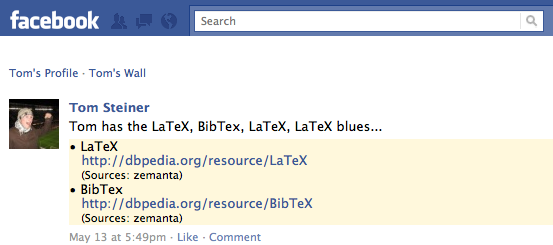
\includegraphics[width=0.75\textwidth]{facebook-swarm-nlp.png}
  \caption[Facebook Swarm NLP browser extension]
    {Facebook Swarm NLP browser extension.
    Extracted named entities have a~pale yellow background.}     
  \label{fig:facebookswarmnlp}
\end{figure}

\subsection{A~Wrapper API for Named Entity Disambiguation}
\label{sec:wrapperapi}

As mentioned before, in order to perform named entity extraction
and disambiguation, we rely on a~wrapper API
that calls existing third-party NLP APIs in the background
and that delivers the combined results of these APIs
in a~consolidated way.
It is  desirable
(i)~to credit back the contribution of each single third-party API
to the joint results, and
(ii)~to track the provenance of the joint results
in order to understand how they were formed.
We will show how these two constraints
can be fulfilled in a~generalizable way
at the concrete example of the wrapper NLP API
used for our browser extensions.

\section{Related Work}

We regard related work from different angles.
First, we look at different approaches
for named entity disambiguation,
which are relevant for adding meaning to microposts.
Second, we look at efforts to mash-up Web services,
which is important for tracking data provenance
when using multiple APIs in combination.

\subsection{Named Entity Disambiguation Using Lexical Databases}

In~\cite{choudhury2009youtubetags},
Choudhury \emph{et~al.}\ describe a~framework for
the semantic enrichment, ranking, and integration
of Web video tags using Semantic Web technologies.
This task is more related to microposts
than it seems at first sight:
video tags can consist of more than one word
and microposts (especially on Twitter) oftentimes consist
of just a~few words.
In order to enrich the typically sparse
user-generated tag space,
metadata like the recording time and location
or the video title and video description are used,
but also social features such as the playlists
where a~video appears in and related videos.
Next, the tags are ranked by their co-occurrence
and in a~final step interlinked with DBpedia~\cite{auer2007dbpedia}
concepts for greater integration with other datasets.
The authors disambiguate the tags based on
WordNet~\cite{miller1995wordnet,fellbaum1998wordnet}
synsets (groups of data elements that are considered
semantically equivalent for the purpose of information retrieval)
if possible, \emph{i.e.},
if there is only one matching synset in WordNet,
the corresponding WordNet URI in DBpedia is selected.
If there are more than one matching synsets,
the tags' and their context tags' similarity is computed
to decide on an already existing tag URI.

\subsection{Named Entity Disambiguation with Semantic Coherence and News Trends}

In~\cite{fernandez2007identityrank},
Fernández \emph{et~al.}\ examine named entity disambiguation
in the context of news annotation.
Their approach consists of three steps:
finding the candidate instances in the NEWS
ontology~\cite{fernandez2010newsontology}
for each entity in a~news item,
ranking these candidate instances
using a~modified version of
PageRank~\cite{brin1998pagerank},
and finally retraining the algorithm
with the journalist's feedback once the process is finished.
The approach first takes into account the number
of occurrences of candidate entities in the past
in order to find news trends,
and second, the occurrences of candidate entities
in past articles in the same categories
in order to find semantic coherences.

\subsection{Named Entity Disambiguation with Disambiguation Dictionaries}

In~\cite{nguyen2008namedentity},
Nguyen \emph{et~al.}\ show how disambiguation dictionaries
can be used to disambiguate entities
using Wikipedia disambiguation pages.
For a~set of entity candidates, all disambiguations are ranked
using tf-idf (or cosine similarity)~\cite{manning2008ir}.
The approach is a~hybrid and incremental process
that utilizes previously identified named entities
and related terms co-occurring with ambiguous names
in a~text for entity disambiguation.

\subsection{Disambiguation with Corpuses and Probability}

Cucerzan shows in~\cite{cucerzan2007largescale}
the use of a~corpus like Wikipedia for entity disambiguation.
The surrounding words of the to-be-disambiguated terms
plus the tags and categories of the related Wikipedia articles
are used to determine semantic coherence and thus
to decide on the most probable entity candidate.
This happens through a~process of heuristically maximizing
the agreement between contextual information
extracted from Wikipedia and the context of a~document.

\subsection{Disambiguation With Search Query Logs}

In~\cite{billerbeck2010rankingentities}, Billerbeck \emph{et~al.}\ use
click graphs and session graphs
of users' search engine sessions
to semantically bridge different queries in order to
retrieve entities for a~concrete entity retrieval query.
Click graphs are created by using queries and URLs as nodes
and connecting and weighting them by their click frequencies.
Session graphs are created by using only queries as nodes
with edges between them if they appear in the same user sessions,
again weighted by co-occurrence frequencies.
An exemplary entity retrieval query is \emph{hybrid cars},
semantically bridgeable queries are consequently \emph{toyota prius},
or \emph{honda civic hybrid}).
These entities are then ranked and returned to the user.

\subsection{Combining Different Web Services and Provenance}

In~\cite{groth2009mashups}, Groth \emph{et~al.}\ describe
how so-called mash-ups can be created in a~dynamic,
just-in-time way, combining data from different data sources
through tools and technologies such as
Yahoo! Pipes,\footnote{\url{http://pipes.yahoo.com/pipes/},
accessed July 15, 2013}
RSS~\cite{cadenhead2006rss}, and APIs.
The authors are driven by the motivation to allow for trust
and confidence in mash-ups, and therefore
consider it critical to be able to analyze the origin
of combined results.
They suggest an approach based on OWL~\cite{mcguinness2004owl}
and XML~\cite{bray2008xml},
with a~focus on process documentation.
However, different from our work, where the goal is to transparently
add provenance data at API invocation time,
their focus is more on overall process documentation
in the context of a~mash-up application.

The focus of Carroll \emph{et~al.}\ in~\cite{carroll2005namedgraphs}
is on the provenance of triples in the Semantic Web world, namely,
for making statements about triples in graphs.
Therefore, the authors introduce the concept of Named Graphs,
an extension to RDF~\cite{klyne2004rdf}.
In contrast to our work, Carroll \emph{et~al.}\ focus
purely on using triples to make statements about triples
(\emph{i.e.}, stay in the RDF world),
whereas our approach uses RDF to make statements
about potentially any API result.
 
Web service specifications in the context of the 
first-generation standards represented by WSDL~\cite{christensen2001wsdl},
SOAP~\cite{gudgin2007soap}, and UDDI~\cite{sabbouh2001uddi}
are occasionally referred to collectively as \emph{WS-*}.
In the \emph{WS-*} world, BPEL4WS, described by
Curbera \emph{et~al.}\ in~\cite{curbera2003bpel4ws}
provides a~formal language for the specification of
business processes and business interaction protocols.
This allows for the combination of several APIs.
However, it does not credit back concrete outputs of a~combined API
to the underlying APIs.

\section{Structuring Unstructured Textual Data} 
\label{sec:structuring}

When we speak of adding structure to unstructured textual data,
we mean the process of extracting the main concepts
in the form of named entities from a~given text
and the process of disambiguating those named entities,
\emph{i.e.}, the removal of uncertainty of meaning from
an ambiguous named entity like \emph{Barcelona},
which can stand for the football club, or the city of Barcelona.
An \emph{entity} is defined by
WordNet~\cite{miller1995wordnet,fellbaum1998wordnet}
as \textit{``that which is perceived or known or inferred
to have its own distinct existence (living or nonliving)''}. 
Typically, named entities from a~text can be persons, companies,
organizations, geographies, but also things like quantities,
expressions of time, books, albums, authors, \emph{etc.}
The extraction of named entities is commonly based on
Natural Language Processing (NLP) combined with Machine Learning.

\subsection{Natural Language Processing Services}
\label{sec:nlp-services}

WordNet~\cite{miller1995wordnet,fellbaum1998wordnet}
defines \emph{Natural Language Processing} as
\textit{``the branch of information science that deals with
natural language information''}.
From the many NLP toolkits available,
hereafter, we list some NLP Web services
that link to datasets in the
Linking Open Data
cloud~\cite{bizer2011statelodcloud,cyganiak2011lodcloud}
in order to disambiguate named entities.

\subsubsection{OpenCalais}\label{sec:opencalais}

The OpenCalais%
\footnote{\url{http://www.opencalais.com/documentation/opencalais-documentation},
accessed July 15, 2013}
Web service automatically creates rich semantic metadata
for textual documents.
Using Natural Language Processing (NLP),
machine learning, and other methods, OpenCalais analyzes documents
and finds the entities within, and also returns the facts and
events hidden within them.
OpenCalais is the only of the examined Web services
that provides details on occurrences in concrete sections
of the submitted coherent text.
This allows for the exact matching of the location in the text
where a~certain entity is detected.
This is especially useful as OpenCalais
is also oftentimes capable of recognizing references
within the text to prior discovered entities
(for example, in the following text,
\emph{he} is mapped back to Obama: \textit{``\emph{Obama}
thanked people for their work in ensuring the victory.
\emph{He} also thanked his family.''}).
An OpenCalais response consists of three parts:

\begin{itemize}
  \itemsep0em
  \item a~list of topics that the text is categorized in
  \item a~list of concrete entities that occur in the text
  \item a~list of social concept tags
\end{itemize}

The problem with the extracted entities is
that they are not always uniquely disambiguated.
An example is the named entity
represented by the URL \url{http://d.opencalais.com/pershash-1/cf42394f-4ae9-3e8e-958a-088149c86565.html}
that represents the concept of an entity of type \texttt{person}
named \emph{Barack Hussein Obama}.
However, a~\texttt{person}-type \emph{Barack Obama} entity from the same document is also represented by the URL
\url{http://d.opencalais.com/pershash-1/cfcf1aa2-de05-3939-a7d5-10c9c7b3e87b.html}
Other services successfully disambiguated both occurrences and
recognized them to stand for the same person, President Obama.
A~second issue is that only a~tiny fraction of the returned
entities link to other data sources in the
LOD cloud~\cite{bizer2011statelodcloud,cyganiak2011lodcloud}.
In order to discover links to the LOD cloud,
each returned entity URL has to be retrieved at the expense
of an HTTP request and the returned RDF has to be checked
for said links.

\subsubsection{AlchemyAPI}

AlchemyAPI\footnote{\url{http://www.alchemyapi.com/api/entity/},
accessed July 15, 2013}
is capable of identifying people, companies, organizations,
cities, geographic features, and other typed entities within
textual documents.
The service employs statistical algorithms and NLP
to extract semantic richness embedded within text.
AlchemyAPI differentiates between entity extraction and
concept tagging.
AlchemyAPI's concept tagging API is capable of abstraction, \emph{i.e.},
understanding how concepts relate and tag them accordingly
(``Hillary Clinton'', ``Michelle Obama'', and ``Laura Bush" are all
tagged as ``First Ladies of the United States'').
In practice, the difference between named entity extraction
and concept tagging is subtle.
In consequence, we treat entities and concepts the same.
Overall, AlchemyAPI results are very accurate
and in the majority of cases well interlinked
with members of the LOD cloud,
among others with DBpedia~\cite{auer2007dbpedia},
OpenCyc~\cite{lenat1995cyc},
and Freebase~\cite{markoff2007freebase}.
AlchemyAPI also provides links to other data sources, however,
sometimes the returned URLs result in \texttt{404 Not found}.
One example that we came across during our tests was the URL
\url{http://umbel.org/umbel/ne/wikipedia/George\_W.\_Bush.rdf}, which should represent the concept of the person George W. Bush.
The URL does serve as a~Semantic Web identifier, however, 
harms the third Linked Data principle,
as outlined in \autoref{sec:linked-data-principles}.
AlchemyAPI also oftentimes returns thematically closely related,
but for a~concrete text not directly relevant entities
beyond the abstract concepts from its concept tagging service,
for example, in a~text about the CEO of a~given company,
the name of the CEO of one of its competitors.

\subsubsection{Zemanta}

Zemanta\footnote{\url{http://developer.zemanta.com/docs/},
accessed July 15, 2013}
allows developers to query the service for contextual metadata
about a~given text.
The returned components currently span four categories:
articles, keywords, photos, in-text links, and
optional component categories.
The service provides high quality entities that are linked
to well-known datasets of the LOD cloud, \emph{e.g.},
DBpedia or Freebase.
Zemanta convinces through very accurate entity disambiguation
and thus high precision, however, at the cost of recall.
Where other services return named entities of lower precision,
the design objectives of Zemanta instead seem to prefer
not to return anything over returning returning low-precision results.

\subsubsection{DBpedia Spotlight}

DBpedia Spotlight~\cite{mendes2011dbpediaspotlight}
is a~tool for annotating mentions of DBpedia resources in text,
providing a~solution for linking unstructured information sources
to the LOD cloud through DBpedia.
DBpedia Spotlight performs named entity extraction,
including entity detection and disambiguation
with adjustable precision and recall.
DBpedia Spotlight allows users to customize the annotations
to their specific needs through the DBpedia
Ontology\footnote{\url{http://wiki.dbpedia.org/Ontology},
accessed July 15, 2013}
and quality measures such as prominence, topical pertinence,
contextual ambiguity, and disambiguation confidence.

\subsection{Machine Translation}
\label{sec:machine-translation}

Social networking happens at a~global scale.
In consequence, many microposts are authored
in languages different from English.
In order to still make sense out of those microposts,
we apply machine translation to translate non-English microposts
to English.
We use the Google Translate
API,\footnote{\url{https://developers.google.com/translate/v2/getting_started},
accessed July 15, 2013}
which, if the source language parameter is left blank,
tries to first detect the source language,
and subsequently translates the micropost to English.

\subsection{Part-of-Speech Tagging}
\label{sec:part-of-speech-tagging}

Our processing chain supports part-of-speech (POS) tagging
based on a~Brill POS tagger~\cite{brill1992pos} adapted for JavaScript.
Brill taggers work by assigning tags to each word and then changing them
using a~set of predefined rules.
In an initial run, if a~word is known, the tagger
first assigns the most frequent tag,
or, if a~word is unknown, it naively assigns the tag ``noun'' to it.
By applying the processing rules over and over again and
changing the incorrect tags, a~sufficiently high accuracy is achieved.
In the current processing chain, POS tagging does not yet
play an active role,
however, we aim for leveraging the additional data
for better micropost analysis in the future.

\section{Consolidating Named Entity Disambiguation Results} 
\label{sec:consolidate}

In this section, we motivate the use of multiple
named entity disambiguation Web services in \emph{parallel}
with the objective of obtaining named entity candidates
for a~textual document such as a~micropost.
The task of evaluating and aligning named entity extraction and
disambiguation APIs and their typed output
has been formally addressed by Rizzo \emph{et~al.}\ in
the context of the NERD
framework~\cite{rizzo2011nerd,rizzo2012nerd}.
We have decided for a~type-agnostic approach,
which we motivate in the following.

\subsection{Identity Links on the Semantic Web}
\label{sec:sameasorg}

From the considered services, only OpenCalais returns data in its
own namespace (\url{http://d.opencalais.com/*}), which is
interlinked with other datasets in the LOD cloud,
however, not in all cases.
In contrast, all other services return results either directly
in the DBpedia namespace (\url{http://dbpedia.org/resource/*}),
as in the case of DBpedia Spotlight,
or in the DBpedia namespace together with other
well interlinked LOD cloud dataset namespaces like Freebase
(\url{http://rdf.freebase.com/rdf/*}) in the cases of
AlchemyAPI and Zemanta.

In order to address the problem of different namespaces in results,
an approach as presented by Glaser \emph{et~al.}\ 
in~\cite{glaser2009sameas} based on \texttt{owl:sameAs} links
could be used.
In practice, however, while many resources in the Linked Data
world are marked as equivalent to each other,
the quality of such equivalence links is not always optimal.
An example of a~good equivalence link is shown in \autoref{code:sameas}.

\begin{lstlisting}[caption={Example of a~good equivalence link},
  label={code:sameas},
  escapechar=§]
<http://dbpedia.org/resource/Barack_Obama> §\linewrap§
  <http://www.w3.org/2002/07/owl#sameAs> §\linewrap§
  <http://rdf.freebase.com/rdf/en.barack_obama> .
\end{lstlisting}

\noindent As Halpin \emph{et~al.}\ show
in a~study~\cite{halpin2010owlsameas}, the problem
with \texttt{owl:sameAs} is that people tend to use it
in different ways with different intentions.
In~\cite{halpin2010owlsameas},
the authors differentiate between four separate usage styles,
ranging from expressing loose relatedness
to strict equivalence.
Despite the different intentions, people tend to incorrectly use
\texttt{owl:sameAs} habitually, according to the study.
Inference is thus problematic, if not impossible,
when the intention of the link creator of the particular
\texttt{owl:sameAs} link is unknown.

\subsection{Linked Data Principles Applied}

We recall the Linked Data principles, that were outlined
in \autoref{sec:linked-data-principles}.
In order to represent extracted named entities from
social network microposts in an unambiguous way,
we apply the Linked Data principles
by representing named entities in microposts with HTTP URIs
that can be dereferenced for retrieving the corresponding information.
This is taken care of by the third-party NLP APIs
that we use for our experiments, namely OpenCalais,
Zemanta, DBpedia Spotlight, and AlchemyAPI.
These APIs take a~textual document as an input,
perform named entity extraction and disambiguation on it,
and finally link the detected named entities back
into the LOD cloud.
We use these APIs in parallel and by combining their results
aim for the emergence effect%
\footnote{Aristotle, Metaphysics, Book H 1045a 8--10}
in the sense of Aristotle:
\textit{``the totality is not, as it were, a~mere heap,
but the whole is something besides the
parts''}.

We recall the wrapper API described in \autoref{sec:wrapperapi}
that calls third-party NLP Web services
in order to return a~combined result of consolidated entities.
All NLP Web services return lists of entities with
their respective types and/or subtypes, names,
relevance, and URIs that interlink the entity in question
with the LOD cloud.
The problem is that each service has implemented
its own typing system.
Providing mappings for all of them
is a~time-consuming, cumbersome task.
While Rizzo \emph{et~al.}\ have defined mappings in the context
of the NERD framework~\cite{rizzo2011nerd,rizzo2012nerd},
we decided for a~different approach.
As all services provide links into the LOD cloud,
the desired typing information can be retrieved from there
in a~true Linked Data manner if need be.

We illustrate the approach with an example:
\textit{``Google Inc.\ is an American multinational corporation
which provides Internet-related products and services,
including Internet search, cloud computing, software and 
advertising technologies.''}
If we use the just mentioned text
as an input for the NLP wrapper API,
among others, we expect to retrieve the named entity for the
company Google, represented by, for example, the URL
\url{http://dbpedia.org/resource/Google} as an output.

\autoref{code:googlezemanta} shows the output
of just Zemanta in isolation,
\autoref{code:googlealchemyapi} shows the output
of just AlchemyAPI in isolation,
and finally, \autoref{code:googlecombined} shows the consolidated
output of the two named entity recognition APIs together. 
In this example, the entity names differ (``Google Inc.''
vs. ``Google''). However, going down the list of URLs for
each entity from the two services, the consolidation algorithm
matches via the URL \url{http://dbpedia.org/resource/Google}.
Given the different two entity names (``Google Inc.'' vs.\
``Google''), the consolidated name is then an array of all
detected names.
Each service already includes a~relevance score ranging from
0 (irrelevant) to 1 (relevant).
The consolidated relevance is calculated via the
averaged relevance scores of both services.
While there may be different definitions of relevance
applied by each service and given
that these differences are not disclosed,
the arithmetic mean is a~pragmatic way to deal with the situation,
especially as all services use relevance scores between 0 and 1.
We maintain provenance metadata for each URI
on the JSON representation,
as can be seen in \autoref{code:googlecombined}.
Finally, we repeat the process for all other services.

\newpage

\begin{lstlisting}[caption={Output of Zemanta in isolation},
  label={code:googlezemanta}]
[
  {
    "name": "Google Inc.",
    "relevance": 0.972007,
    "uris": [
      {
        "uri": "http://rdf.freebase.com/ns/en/google",
        "source": "zemanta"
      },
      {
        "uri": "http://dbpedia.org/resource/Google",
        "source": "zemanta"
      }
    ],
    "source": "zemanta"
  }
]
\end{lstlisting}

\begin{lstlisting}[caption={Output of AlchemyAPI in isolation},
  label={code:googlealchemyapi}]
[
  {
    "name": "Google",
    "relevance": 0.535781,
    "uris": [
      {
        "uri": "http://dbpedia.org/resource/Google",
        "source": "alchemyapi"
      },
      {
        "uri": "http://rdf.freebase.com/ns/guid.9202a8c04000641f800000000042acea",
        "source": "alchemyapi"
      }
    ],
    "source": "alchemyapi"
  }
]
\end{lstlisting}

\newpage

\begin{lstlisting}[caption={
   [Consolidated output of two named entity recognition APIs]
   {Consolidated output of two named entity recognition APIs,
    namely Zemanta and AlchemyAPI}
  },
  label={code:googlecombined}]
[
  {
    "name": [
      "Google",
      "Google Inc."
    ],
    "relevance": 0.753894,
    "uris": [
      {
        "uri": "http://rdf.freebase.com/ns/en/google",
        "source": "zemanta"
      },
      {
        "uri": "http://dbpedia.org/resource/Google",
        "source": "zemanta"
      },
      {
        "uri": "http://rdf.freebase.com/ns/guid.9202a8c04000641f800000000042acea",
        "source": "alchemyapi"
      }
    ],
    "source": "zemanta,alchemyapi"
  }
]
\end{lstlisting}

\section{Tracking Provenance With Multiple Sources}                    \label{sec:tracking}

As outlined before, we use several APIs in combination
in order to add meaning to social network microposts.
Extracted named entities from a~micropost can in consequence
be the result of up to four agreeing (or disagreeing) API calls.

\subsection{The Need for Providing Provenance Metadata}

Hartig \emph{et~al.}\ mention in~\cite{hartig2010provenance}
reasons that justify the need for provenance metadata.
Among these reasons are linked dataset replication and distribution
on the Web with not necessarily identical namespaces:
based on the same source data, different publishers can
create diverging copies of a~linked dataset
with different levels of interconnectedness.
We add to this the automated conversion of unstructured data
to Linked Data with heuristics,
where extracted entities---albeit consolidated
and backed by different data sources---might still be wrong.
Especially with our wrapper approach,
it is desirable to be able to track back to the concrete source
where a~certain piece of information came from.
This enables
(i) to correct the error at the root of our API
(fighting the cause) or
(ii) to correct the concrete error in an RDF annotation
(fighting the symptom), and
(iii) to judge the trustworthiness and quality of a~dataset,
which represents the most important reason.

In order to track the contributions of the various sources,
we have opted to use the Provenance
Vocabulary~\cite{hartig2012provenance}
by Hartig and Zhao with the prefix \texttt{prv},
the HTTP Vocabulary in RDF~\cite{koch2011http}
by Koch \emph{et~al.}\ with prefix \texttt{http},
and a~vocabulary for representing content in
RDF~\cite{koch2011content}
by the same authors with prefix \texttt{cnt}.
We have chosen the HTTP Vocabulary in RDF for the fact that
it is a~W3C Working Draft developed by the
Evaluation and Repair Tools Working Group (ERT WG),
which is part of the World Wide Web Consortium (W3C)
Web Accessibility Initiative (WAI).
The Provenance Vocabulary was chosen because of its existing
deployment in several projects, such as
Pubby,\footnote{\url{http://wifo5-03.informatik.uni-mannheim.de/pubby/},
accessed July 15, 2013}
Triplify,\footnote{\url{http://triplify.org/Overview},
accessed July 15, 2013}
and D2R
Server.\footnote{\texttt{http://wifo5-03.informatik.uni-mannheim.de/bizer/d2r-server/publishing/},
accessed July 15, 2013}

While our wrapper API supports two output formats
(\texttt{application/json} and\linebreak \texttt{text/turtle}),
we have added provenance information exclusively to the
\texttt{text/turtle} variant.
In order to represent the extracted named entities in a~micropost,
we use the Common Tag vocabulary~\cite{tori2009commontag}.
A~micropost is \texttt{ctag:tagged} with a~\texttt{ctag:Tag},
which consists of a~textual \texttt{ctag:label} and a~pointer
to a~resource that specifies what the label \texttt{ctag:means}.
The Common Tag vocabulary is well-established and developed by
both industry and academic partners.
In order to make statements about a~bundle of triples,
we group them in a~named graph.
We use the TriG~\cite{bizer2007trig} syntax,
an example can be seen in \autoref{code:trig}.

\begin{lstlisting}[caption={Example named graph in TriG syntax},
  label={code:trig}]
:G = {
  <https://www.facebook.com/Tomayac/posts/10150175940867286> ctag:tagged [
      a~ctag:Tag ;
      ctag:label "BibTeX" ;
      ctag:means <http://dbpedia.org/resource/BibTeX>
    ] .
} .
\end{lstlisting}

\subsection{The Provenance Vocabulary}
\label{sec:provenance}

In this section, we outline the required steps
in order to make statements about the provenance
of a~group of triples contained in a~named graph
\texttt{:G} that was generated using several HTTP \texttt{GET}
requests to third-party APIs.
We use the Provenance Vocabulary~\cite{hartig2012provenance} with
prefix \texttt{prv}, the HTTP Vocabulary in RDF~\cite{koch2011http}
with prefix \texttt{http},
the Identity of Resources on the Web ontology%
\footnote{\url{http://www.ontologydesignpatterns.org/ont/web/irw.owl\#},
accessed July 15, 2013} (IRW)
with the prefix \texttt{irw},
and the Representing Content in RDF
vocabulary~\cite{koch2011content} with prefix \texttt{cnt}.

As a~first step, we state that \texttt{:G} is both a~\texttt{prv:DataItem}
and an \texttt{rdfg:Graph}.
\texttt{:G} is \texttt{prv:createdBy} the process of
a~\texttt{prv:DataCreation}.
This \texttt{prv:DataCreation} is \texttt{prv:performedBy}
a~\texttt{prv:NonHumanActor},
a~\texttt{prvTypes:DataProvidingService}
to be precise (simplified as
\texttt{http://tomayac.no.de/entity-extraction/combined}
in \autoref{code:provenance}).
This service is \texttt{prv:operatedBy} a~human,
in the concrete case ourselves,
(\texttt{http://tomayac.com/thomas\_steiner.rdf\#me}).
Time is important for provenance,
so the \texttt{prv:performedAt} date of
the \texttt{prv:DataCreation}
needs to be saved.
During the process of the \texttt{prv:DataCreation}
there are \texttt{prv:usedData},
which are \texttt{prv:retrievedBy} a~\texttt{prv:DataAcess}
that is \texttt{prv:performedAt} a~certain time,
and \texttt{prv:performedBy} a~non-human actor
(our API) that is \texttt{prv:operatedBy}
the same human as before.
For the \texttt{prv:DataAccess}
(there is one for each involved API),
we \texttt{prv:accessedService} from
a~\texttt{prv:DataProvidingService} of which we
\texttt{prv:accessedResource} that is available at
a~certain \texttt{irw:WebResource}.
Therefore, we \texttt{prvTypes:exchangedHTTPMessage} which is an
\texttt{http:Request} using \texttt{http:httpVersion} ``1.1''
and the \texttt{http:methodName} ``GET''.

\subsection{Provenance RDF Overview}

This section provides a~shortened overview of the provenance RDF
serialized in Turtle syntax for a~micropost that was automatically
tagged with the label ``BibTeX''
and the assigned meaning
\url{http://dbpedia.org/resource/BibTeX}.
The named graph \texttt{:G} in the first part
of \autoref{code:provenance}
contains the absolute data (the fact that the micropost with
the URL
\url{https://www.facebook.com/Tomayac/posts/10150177486072286}
is tagged with the label ``BibTeX'', which is represented by
the HTTP URL \url{http://dbpedia.org/resource/BibTeX}).
The second part with metadata about \texttt{:G} says that
these facts were generated via two calls,
one using the HTTP method \texttt{GET},
and the other \texttt{POST}.
It is to be noted that statements
such as in \autoref{code:provenance} 
refer to the triple objects as an identifier for a~Web resource
(where the Web resource is a~representation of the result of the
API call at the time where it was \texttt{prv:performedAt}).
As provenance metadata always refers to the time context
in which a~certain statement was made,
it is essentially unimportant
what representation the resource returns in future.

\begin{lstlisting}[caption={[Shortened overview of the provenance
       RDF in Turtle syntax]{Shortened overview of the provenance
       RDF in Turtle syntax for an automatically annotated
       micropost}},
  label={code:provenance},escapechar=§]
:G = {
  <https://www.facebook.com/Tomayac/posts/10150177486072286> ctag:tagged [
     a ctag:Tag ;
     ctag:label "BibTeX" ;
     ctag:means <http://dbpedia.org/resource/BibTeX> ;
  ] .
} .


:G
  a prv:DataItem ;
  a rdfg:Graph ;
  prv:createdBy [
    a prv:DataCreation ;
    prv:performedAt "2011-05-20T15:06:30Z"^^xsd:dateTime ;
    prv:performedBy <http://tomayac.no.de/entity-extraction/combined> ;
    prv:usedData [
      prv:retrievedBy [
        a prv:DataAcess ;
        prv:performedAt "2011-05-20T15:06:30Z"^^xsd:dateTime ;
        prv:performedBy <http://tomayac.no.de/entity-extraction/combined> ;
        prv:accessedService <http://spotlight.dbpedia.org/rest/annotate> ;
        prv:accessedResource
          <http://spotlight.dbpedia.org/rest/annotate?text=Tom%20has%20... §\linewrap§
              blues&confidence=0.4&support=20> ;
        prvTypes:exchangedHTTPMessage [
          a http:Request ;
          http:httpVersion "1.1" ;
          http:methodName "GET" ;
          http:mthd <http://www.w3.org/2008/http-methods#GET> ;
        ] ;
      ] ;
    ] ;
    prv:usedData [
      prv:retrievedBy [
        a prv:DataAcess ;
        prv:performedAt "2011-05-20T15:06:41Z"^^xsd:dateTime ;
        prv:performedBy <http://tomayac.no.de/entity-extraction/combined> ;
        prv:accessedService <http://api.zemanta.com/services/rest/0.0/> ;
        prv:accessedResource <http://api.zemanta.com/services/rest/0.0/> ;
        prvTypes:exchangedHTTPMessage [
          a http:Request ;
          http:httpVersion "1.1" ;
          http:methodName "POST" ;
          http:mthd <http://www.w3.org/2008/http-methods#POST> ;
          http:headers (
            [
              http:fieldName "Content-Type" ;
              http:fieldValue "application/x-www-form-urlencoded" ;
            ]   
          )
          http:body [
            a cnt:ContentAsText ;
            cnt:characterEncoding "UTF-8" ;
            cnt:chars """method=zemanta.suggest_markup §\linewrap§
            &api_key=Your_API_Key §\linewrap§
            &text=Tom%20has%20...blues §\linewrap§
            &format=json §\linewrap§
            &return_rdf_links=1""" ;
          ] ;
        ] ;
      ] ;
    ] ;
  ] .
\end{lstlisting}

\section{Conclusions}                                                        

In this chapter, we have shown how the Provenance
Vocabulary can be used to keep track of the original
third-party Web service calls that led to the consolidated
results. These references to the original calls
are to be understood as the identification of Web resources,
\emph{i.e.}, the results of a~request.
We have shown how a~concrete multi-source Web service can
automatically maintain provenance metadata
both for entirely machine-generated content,
but also for partly (or completely) human-generated content.
Being able to track back the origin of a~triple
is of crucial importance,
especially given the network effect which is one of the
Linked Data benefits.
The generated triples are very verbose,
and in consequence stating even simple facts like
that a~combined result is based on two separate sub-results
takes up a~lot of space.
The verbosity is mainly due to the used vocabularies,
the Provenance Vocabulary and the HTTP Vocabulary in RDF.

Future work will focus on exploring ways
to drastically simplify the annotations in order to obtain
less verbose provenance descriptions.
While it is always easier to come up with a~specialized vocabulary
that does one task well, broader reuse and acceptance
can be gained by reusing existing vocabularies.

\section*{Chapter Notes}
This chapter is partly based on the following publications.
%\cite{steiner2011addingmeaning,steiner2013addingmeaning,van2013named}.

\begin{itemize}
  \item \bibentry{steiner2011addingmeaning}.
  \item \bibentry{steiner2013addingmeaning}.
  \item \bibentry{van2013named}.  
\end{itemize}

\bibliographystyle{plainnat}
\clearpage
\bibliography{backmatter/references}

\chapter{Media Item Extraction}
\label{cha:media-item-extraction}

% the code below specifies where the figures are stored
\ifpdf
    \graphicspath{{5_media_item_extraction/figures/PNG/}{5_media_item_extraction/figures/PDF/}{5_media_item_extraction/figures/}}
\else
    \graphicspath{{5_media_item_extraction/figures/EPS/}{5_media_item_extraction/figures/}}
\fi

\section{Introduction}

Before the rise of social networks,
event coverage was mostly an affair of professional news agencies.
The widespread availability of mobile phones
with higher resolution cameras has transformed
citizens into witnesses who are used to comment
and share media illustrating events on social networks.
Some examples with global impact
include the shootings in
Ut{\o}ya,\footnote{\url{http://en.wikipedia.org/wiki/2011_Norway_attacks},
accessed July 15, 2013}
which first appeared on Twitter,
the capture and arrest of Muammar
Gaddafi,\footnote{\url{http://en.wikipedia.org/wiki/Death_of_Muammar_Gaddafi},
accessed July 15, 2013}
which first appeared on YouTube,
or the emergency ditching of a~plane in the Hudson
river,\footnote{\url{http://en.wikipedia.org/wiki/US_Airways_Flight_1549},
accessed July 15, 2013}
which first appeared on Twitpic.
Some news
communities\footnote{\url{http://www.citizenside.com/},
accessed July 15, 2013}
have even specialized in aggregating and brokering
such user-generated content.
Events, such as sports matches or concerts are
largely illustrated by social media,
albeit distributed over many social networks.

In this chapter, we tackle the challenge of reconciling
social media data that illustrates known events,
but that is spread over various social networks,
all with the objective of creating visual event summaries.
We propose a~social-network-agnostic
approach for the extraction of photos and videos covering events.
We want to emphasize that in this chapter we do \emph{not}
put the focus on event detection (we have done that in \autoref{cha:eventdetection}).
The events we are dealing with in this chapter
were known beforehand and we use specific
human-chosen search terms to find illustrating media.

We first recall the definitions previously made in
\autoref{sec:definition} and add formal definitions
of the terms \emph{event},
\emph{media item extraction},
\emph{Application Programming Interface},
and \emph{Web scraping}.

\begin{description}
  \item[Social Network:]
       A~social network is an online service or media platform
       that focuses on building and reflecting
       relationships among people
       who share interests and/or activities.
  \item[Media Item:]
       A~media item is defined as
       a~photo\footnote{We choose the term \emph{photo}
       over the term \emph{image} as
       Facebook, Twitter, and \googleplus use it}
       or video file that is publicly shared or published
       on at least one social network.
  \item[Micropost:]
       A~micropost is defined as a~textual status message
       on a~social network
       that can optionally be accompanied by a~media item.
  \item[Event:]
       An event is defined as a~phenomenon that has happened
       or that is scheduled to happen.
       It is an observable occurrence grouping persons,
       places, times, and activities while being often
       documented by people through different media~%
       \cite{liu2011events}.
  \item[Media Item Extraction:]
       The process of leveraging search functionalities of
       social networks to find references to media items,
       which allows for storing those media items in binary form.
  \item[Application Programming Interface (API):]
       An API is a~programmatic specification intended to be used
       as an interface by software components on client and server
       to communicate with each other.
  \item[Web scraping]
       The term Web scraping means the process of
       automatedly extracting information from Web pages.
       Web scraping involves practical solutions based on
       existing technologies that are often entirely \emph{ad hoc}.
       Examples of such technologies are regular expressions,
       Document Object Model (DOM)
       parsing~\cite{lehors2004dom},
       or CSS selectors~\cite{hunt2012cssselectors}.
       The difference between \emph{Web scraping}
       and the related concept of \emph{screen scraping}
       is that screen scraping relies on the visual layout of a~Web page,
       while Web scraping relies on the textual
       and/or hierarchical structure.
\end{description}

\section{Related Work}

Related work covers research
that aims to collect, align, and organize media
for trends or events.
Liu \emph{et~al.}\ combine semantic inferencing and visual analysis
to automatically find media to illustrate
events~\cite{liu2011events}.
They interlink large datasets of event metadata
and media with the Linking Open Data
Cloud~\cite{bizer2011statelodcloud,cyganiak2011lodcloud}.
In~\cite{liu2011socialmedia}, they show how visual summaries
of past events providing viewers with a~more compelling feeling
of the event's atmosphere can be created
based on a~method to automatically detect and identify events
from social media sharing websites.
Approaches to alignment use visual, temporal,
and spacial similarity measures to map multiple photo streams of
the same events~\cite{yang2011photostream}.
Other ways to collect and order media from social networks use
media-driven metadata such as geospatial
information~\cite{crandall2009mappingphotos}.
Becker \emph{et~al.}\ show in~\cite{becker2010eventidentification}
how to exploit the rich context associated with social media
content, including user-provided annotations
and automatically generated information.
Using this rich context, they define similarity metrics
to enable online clustering of media to events.
In~\cite{becker2012plannedevents}, the same authors develop
recall-oriented query formulation strategies
based on noisy event metadata
from event aggregation platforms.

\section{Social Networks and Media Items}                                    \label{sec:social-networks}

Most social networks offer a~search functionality that allows for
content to be retrieved based on search terms,
with or without more advanced search operators
such as exclusion, inclusion, phrase search, \emph{etc.}
Each social network has special constraints
regarding the supported search operators or filtering options.

Social networks are often perceived as
\emph{walled gardens}~\cite{simonds2008walledgarden}
due to the full control of the network operator
over content and media on the social network in question,
oftentimes accessible exclusively by social network members.
This network lock-in effect was excellently illustrated
by David Simonds in a~cartoon that first appeared
in the English-language weekly news and
international affairs publication \emph{The Economist},
reproduced in \autoref{fig:walled-gardens}.
While some social networks (\emph{e.g.}, Twitter)
have full read and write access via specified APIs,
other social networks (\emph{e.g.}, \googleplus)
currently only have read API access.
In some cases, however, API access is limited,
so that not all desired pieces of information is exposed
(\emph{e.g.}, view counts with Img.ly),
which forces people interested in that data
to fall back to Web scraping.
It is to be noted that if the directives in the 
\texttt{robots.txt} file are respected,
Web scraping \emph{per~se} is not an illegal practice,
as only public information is being accessed,
comparable to the level of access that common Web search engines have.
The Robot Exclusion Standard,
also referred to as \texttt{robots.txt} protocol,
is a~widely respected convention to prevent cooperating Web crawlers
and other Web robots
from accessing all or part of a~website
that is otherwise publicly viewable.

\begin{figure}[!ht]
  \centering
  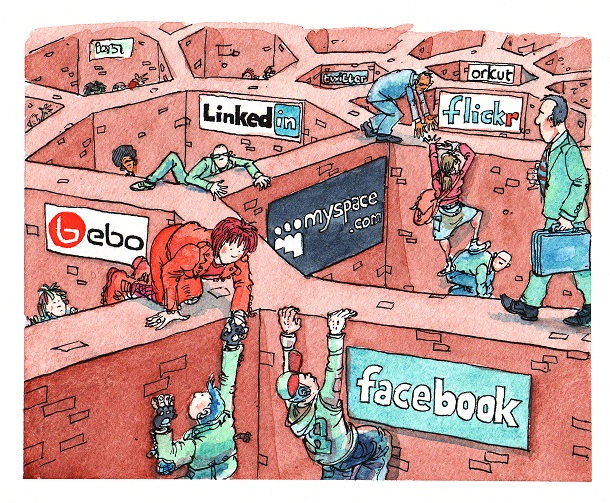
\includegraphics[width=0.7\linewidth,
    trim=16px 17px 12px 15px,clip]{davidsimonds.jpg}
  \caption[Social networks as walled
    gardens illustrated by David Simonds]
    {Social networks as walled gardens illustrated by David Simonds}
  \label{fig:walled-gardens}
\end{figure}

\section{Media Extractor}
\label{sec:media-extractor}

In this section, we first introduce a~common data format
that we have developed as an abstraction layer on top of the native
data formats used by the considered social networks.
We then explain the architecture
of different kinds of media item extractors.
Finally, we describe the processing steps
that we apply to each extracted media item.

\subsection{Abstraction Layer Data Format}
\label{sec:data-format}

Each social network uses a~different data representation schema.
While all social networks with API access are
JSON-based~\cite{crockford2006json}, the differences in both
supported social network features and media item support level,
as was outlined in detail in
\autoref{sec:description-of-popular-social-networks} and
\autoref{sec:classification-of-social-networks},
are also reflected in the returned JSON data.
We therefore propose a~common abstraction layer
on top of the native data formats of all considered social networks.
It is in the nature of any abstraction
that it can only represent the
greatest common divisor of all social networks.
We show the abstraction layer in the following
with the help of a~concrete example,
stemming from a~query to the media extractor
that will be explained in more detail
in the upcoming \autoref{sec:media-item-extractors}.
The media extractor was used to query for media items
that match the search term \emph{hamburg}.
\autoref{code:facebook} shows sample output of the media extractor
for a~Facebook post, which was processed
with named entity extraction and disambiguation
as was detailed in \autoref{cha:micropost-annotation}.

\begin{description}
  \itemsep0em
  \item[\texttt{mediaUrl}] Deep link to a~media item
  \item[\texttt{posterUrl}] Deep link to a~thumbnail for photos
    or still frame for videos
  \item[\texttt{micropostUrl}] Deep link to the micropost on
    the social network
  \item[\texttt{micropost}] Container for a~micropost
  \begin{description}
    \item[\texttt{html}] Text of the micropost,
      possibly with HTML markup
    \item[\texttt{plainText}] Text of the micropost with
      potential HTML markup removed
    \item[\texttt{entities}] Extracted and disambiguated
      named entities from the micropost text
  \end{description}
  \item[\texttt{userProfileUrl}] Deep link to the user's
    profile on the social network
  \item[\texttt{type}] Type of the media item,
    can be \texttt{photo} or \texttt{video}
  \item[\texttt{timestamp}] Number of milliseconds between
    1 January 1970 00:00:00 UTC and the moment
    when the micropost was published
  \item[\texttt{publicationDate}] Date in ISO 8601
    format (YYYY-MM-DDTHH:MM:SSZ) when the micropost was published
  \item[\texttt{socialInteractions}] Container for social
    interactions
  \begin{description}
  \item[\texttt{likes}] Number of times a~micropost was liked, or
    \texttt{unknown}
  \item[\texttt{shares}] Number of times a~micropost was shared, or
    \texttt{unknown}
  \item[\texttt{comments}] Number of comments a~micropost
    received, or \texttt{unknown}
  \item[\texttt{views}] Number of views a~micropost reached, or
    \texttt{unknown}
  \end{description}
\end{description}

\begin{lstlisting}[caption={[Sample output of the media extractor]{Sample output of the media extractor
  showing a~Facebook post processed with named entity extraction
  and disambiguation (slightly shortened for legibility)}},
  label={code:facebook}]
{
  "mediaUrl": "http://video.ak.fbcdn.net/...",
  "posterUrl": "http://external.ak.fbcdn.net/...",
  "micropostUrl": "https://www.facebook.com/permalink.php?story_fbid=
    231781590231029&id=1254772464",
  "micropost": {
    "html": "Videoed between Hamburg and Snyder. Thought I would share.",
    "plainText": "Videoed between Hamburg and Snyder. Thought I would share.",
    "entities": [
      [
        {
          "name": "Hamburg",
          "relevance": 0.82274,
          "uri": "http://dbpedia.org/resource/Hamburg"
        },
        {
          "name": "Snyder",
          "relevance": 0.857,
          "uri": "http://dbpedia.org/resource/Snyder,_Texas"
        }
      ]
    ]
  },
  "userProfileUrl": "https://www.facebook.com/profile.php?id=1254772464",
  "type": "video",
  "timestamp": 1326371479000,
  "publicationDate": "2012-01-12T12:31:19Z",
  "socialInteractions": {
    "likes": 0,
    "shares": 0,
    "comments": 3,
    "views": null
  }
}
\end{lstlisting}

\subsection{Media Item Extractors}
\label{sec:media-item-extractors}

We have developed a~combined media extractor composed of
separate media item extractors for the seven social networks
\googleplus, Myspace, Facebook, Twitter, Instagram, YouTube,
and Flickr, with additional support for the media sharing
platforms Img.ly, Imgur, Lockerz,\footnote{Dysfunctional since April 2013 when the service shut down its API access} Yfrog, MobyPicture, and Twitpic.
The media extractor takes as input a~search term that is relevant
to a~known event, \emph{e.g.}, the term \emph{boston celtics}
for a~recent match of the Basketball team Boston Celtics.
This search term gets forwarded to the search APIs
of all social networks in parallel.
Each social network has a~30 seconds timeout window
to deliver its results.
When the timeout is reached
or when all social networks have responded,
the available results are aligned according to the data format
defined in \autoref{sec:data-format}.
Media items and the relevant metadata like view count, comments,
\emph{etc.}\ are retrieved either directly or via Web scraping.
For some social networks, \emph{e.g.}, Img.ly,
a~combination of Web scraping and API access is required
since the API does not return all necessary fields
of our data format.
While we could default to Web scraping
to obtain all relevant data,
it is more robust to use API access wherever possible
and only fall back to the more brittle Web scraping
for the parts not covered by API access.

\paragraph{Special Role of Twitter:}

Twitter (\autoref{sec:twitter})
plays a~special role, as it can be used as
a third-order support social network,
as was detailed previously in \autoref{sec:classification-of-social-networks}.
This means that the micropost text is located on Twitter,
but the referenced media items are located
on third-party media platforms.
Due to the length limitation for tweets of 140 characters,
short URLs are used on the service.
We search for the search term in question (\emph{e.g.},
following up from the example before, \emph{boston celtics}),
but combine it with the short URL domain parts of
the media platforms.
For example, the short domain URL of the social network Flickr
(\autoref{sec:flickr})
is \url{flic.kr}, where the long domain URL is \url{flicker.com}.
The short domain URL of Instagram
(\autoref{sec:instagram}) is \url{instagr.am},
where the long domain URL is \url{instagram.com}, \emph{etc.}
We have created a~list of all known short domain URLs for the
considered media platforms so that the complete search query
for Twitter is the actual search term,
combined with this list of short domain URLs:

\emph{boston celtics AND (flic.kr OR instagr.am OR ...)}

\noindent The complete data flow is illustrated in the
architectural diagram in \autoref{fig:architecture}.
As a~side note, Twitter on its website now has its own
media extractor based on Twitter Cards~\cite{wang2012twitter}
with support for some of of the media platforms,
however, our own media extractor goes beyond Twitter's offer,
especially since Facebook-owned Instagram's latest break-up with
Twitter.\footnote{\url{http://techcrunch.com/2012/12/05/kevin-systrom-on-pulling-twitter-cards-integration-we-want-images-viewed-on-instagram-com/}, accessed July 15, 2013}

\begin{figure}
  \centering
  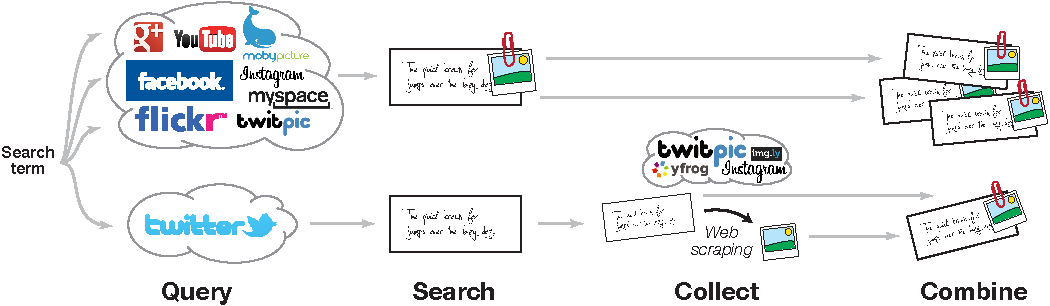
\includegraphics[width=1.0\linewidth]{architecture.pdf}
  \caption[Overview of the media extractor]
    {Overview of the media extractor:
    hybrid approach to the media item extraction task using
    a~combination of API access and Web scraping}
  \label{fig:architecture}
\end{figure}

\section{Evaluation}

We have run experiments in the time period of January 10 to 19, 2012,
during which we have randomly selected nine events
that received broad social media coverage.
For these events, we have collected media items and microposts
using our media extractor.
In the following, we will provide a~short summary of the nine selected events
in order to give the reader the necessary background knowledge.

\begin{description}
  \item[Assad Speech]
       On January 10, 2012, Syrian President Bashar al-Assad
       delivered a~televised talk defending his
       government's actions and motivations, despite world
       pressure on his government for its 10-month
       crackdown on
       protesters.\footnote{\url{http://www.cnn.com/2012/01/10/world/meast/syria-unrest/},
       accessed July 15, 2013}
  \item[CES Las Vegas]
       The International Consumer Electronics Show (CES) is
       a~major technology-related trade show held each January
       in the Las Vegas Convention Center. Not open to the public,
       the Consumer Electronics Association-sponsored show
       typically hosts previews of products and new product
       announcements.
       CES Las Vegas took place from January 11 to 13,
       2012.\footnote{\url{http://www.cesweb.org/},
       accessed July 15, 2013}\\
       \textbf{Cut the Rope Launch:}
       On January 10, 2012 during Microsoft's keynote at CES, the
       HTML5 version of the popular mobile game \textit{Cut the
       Rope} was announced. This is a~sub-event of CES Las
       Vegas.\footnote{\url{http://ces.cnet.com/8301-33377_1-57356403/},
       accessed July 15, 2013}\\
       \textbf{Ubuntu TV Launch:}
       Ubuntu TV by Canonical, based on the user interface Unity,
       is a~variant of the Ubuntu operating system, designed to be
       a~Linux distribution specially adapted for embedded systems
       in televisions. It was announced by Canonical on January
       10, 2012, at
       CES.\footnote{\url{http://www.theverge.com/2012/1/9/2695387/ubuntu-tv-video-hands-on},
       accessed July 15, 2013}
  \item[Costa Concordia Disaster]
       The Costa Concordia is an Italian cruise ship that hit
       a~reef and partially sank on January 13, 2012 off the
       Italian coast. The vessel ran aground at Isola del Giglio,
       Tuscany, resulting in the evacuation of 4,211
       people.\footnote{\url{http://en.wikipedia.org/wiki/Costa_Concordia_disaster},
       accessed July 15, 2013}
  \item[Dixville Notch]
       Dixville Notch is an unincorporated village in Dixville
       township of Coos County, New Hampshire, USA, best known in
       connection with its longstanding middle-of-the-night vote in
       the U.S. presidential election. In a~tradition that started
       in the 1960 election, all the eligible voters in Dixville
       Notch gather at midnight in the ballroom of The Balsams.
       This year, on January 10, 2012, the voters cast their
       ballots and the polls officially closed one minute
       later.\footnote{\url{http://www.washingtonpost.com/2012/01/09/gIQANslKnP_story.html},
       accessed July 15, 2013}
  \item[Free Mobile Launch]
       Free Mobile is a~French mobile broadband company, part of
       the Iliad group. On January 10, 2012, a~long-awaited mobile
       phone package for \EUR{19.99} with calls included to 40
       countries, texts, multimedia messages and Internet was
       announced by the Iliad group's Chief Strategy Officer
       Xavier
       Niel.\footnote{\url{http://www.nytimes.com/2012/01/11/technology/iliad-takes-aim-at-top-mobile-operators-in-france.html},
       accessed July 15, 2013}
  \item[Blackout SOPA]
       The Stop Online Piracy Act (SOPA) is a~bill of the United
       States proposed in 2011 to fight online trafficking in
       copyrighted intellectual property and counterfeit goods.
       On January 18, the English Wikipedia, and several
       other Internet companies coordinated a~service blackout
       to protest SOPA and its sister bill, the Protect IP Act
       (PIPA).
       Other companies, including Google, posted links and
       photos in an effort to raise
       awareness.\footnote{\url{http://sopablackout.org/learnmore/},
       accessed July 15, 2013}
  \item[Christian Wulff Case]
       Since December 2011, former German President Christian
       Wulff faces controversy over discrepancies in statements
       about a~loan while being governor of Lower Saxony.
       It was revealed that he had applied pressure
       on Springer Press to delay revelations on the issue until
       he was back from a~visit abroad. When Wulff found out that
       a~tabloid was going to break the story, he left a~message
       on their voice mail in which he threatened to take legal
       action.\footnote{\url{http://www.spiegel.de/international/germany/0,1518,804631,00.html},
       accessed July 15, 2013}
\end{description}

\subsection{Dataset}
Our data set contained 448 photos with an average file size of
$\sim$0.7MB and 143 videos.
Some videos are no longer available due to either
account termination or video takedown by the user
(Assad, Dixville).
\autoref{tab:number-media} shows the total
numbers of retrieved photos and videos of the media extractor.
Table cell values marked with $n+$ signify that there were more
results, but that only $n$ results were considered.
We have calculated the precisions for each event for both video
and photo separately; the overall photo precision was $0.73$,
and the overall video precision was $0.54$.
We note that these values were calculated \emph{before}
any pruning step, \emph{i.e.}, before taking into account
the additional textual information from microposts like
potential extracted named entities.
The dataset is very diverse with respect to photo quality,
photo format, and naturally, content.
It ranges from entirely sharp screenshots
in all sorts of formats (\emph{e.g.},
screenshots of the Google homepage for the Blackout SOPA event
to screenshots of a~wide banner advertisement),
over to blurry cell phone photos in standard photo formats
(\emph{e.g.}, photos of the stage
for the Free Mobile Launch event).
\autoref{fig:sequences} shows sample photos for
some of the considered nine events.
We have observed that more than one search session
with different combinations of search terms~%
\cite{becker2010eventidentification,becker2012plannedevents}
is necessary in order to obtain a~satisfactory recall.
Query strategies developed by Becker~\cite{becker2012plannedevents}
that combine different combinations of event title,
event venue, and event city work consistently well.

\begin{sidewaystable}[!ht]
  \centering
  \footnotesize
  \begin{tabular}{|l|c|c|c|c|c|c|c|c|c|c|c|c|c|c|c|c|c|c|}
    \hline
    \multicolumn{1}{|c|}{\textbf{Social}} & \multicolumn{2}{c|}{\textbf{Assad}} & \multicolumn{2}{c|}{\textbf{CES}} &
    \multicolumn{2}{c|}{\textbf{Concordia}} & \multicolumn{2}{c|}{\textbf{Dixville}} & \multicolumn{2}{c|}{\textbf{Free}} &
    \multicolumn{2}{c|}{\textbf{Ropes}} & \multicolumn{2}{c|}{\textbf{SOPA}} & \multicolumn{2}{c|}{\textbf{Ubuntu}} &
    \multicolumn{2}{c|}{\textbf{Wulff}} \\
    \cline{2-19}
    \multicolumn{1}{|c|}{\textbf{Network}} & \textbf{P} & \textbf{V} & \textbf{P} & \textbf{V} & \textbf{P} & \textbf{V} &
    \textbf{P} & \textbf{V} & \textbf{P} & \textbf{V} & \textbf{P} & \textbf{V} & \textbf{P} & \textbf{V} & \textbf{P} &
    \textbf{V} & \textbf{P} & \textbf{V} \\
    \hline
    \textbf{\googleplus} & 3 & 2 & 5 & 3 & 15 & 1 & 4 & 1 & 6 & 0 & 5 & 1 & 5 & 0 & 6 & 1 & 7 & 0\\
    \textbf{Myspace} & 0 & 0 & 0 & 0 & 10+ & 0 & 9 & 0 & 1 & 0 & 6 & 0 & 0 & 0 & 0 & 0 & 8 & 0\\
    \textbf{Facebook} & 0 & 0 & 0 & 1 & 0 & 1 & 0 & 0 & 0 & 0 & 0 & 0 & 0 & 2 & 0 & 0 & 0 & 0\\
    \textbf{Twitter} & 2 & 0 & 2 & 0 & 3 & 0 & 3 & 0 & 2 & 0 & 4 & 0 & 5 & 0 & 0 & 0 & 2 & 0\\
    \textbf{Instagram} & 0 & 0 & 20+ & 0 & 20+ & 0 & 0 & 0 & 20+ & 0 & 20+ & 0 & 20+ & 0 & 0 & 0 & 2 & 0\\
    \textbf{YouTube} & 0 & 10+ & 0 & 10+ & 0 & 10+ & 0 & 3 & 0 & 10+ & 0 & 10+ & 0 & 10+ & 0 & 10+ & 0 & 10+\\
    \textbf{Flickr} & 10+ & 0 & 10+ & 6 & 10+ & 10+ & 10+ & 10+ & 10+ & 0 & 10+ & 10+ & 10+ & 0 & 10+ & 9 & 10+ & 2\\
    \textbf{MobyPic} & 0 & 0 & 1 & 0 & 4 & 0 & 0 & 0 & 2 & 0 & 20+ & 0 & 1 & 0 & 2 & 0 & 3 & 0\\
    \textbf{Twitpic} & 0 & 0 & 20+ & 0 & 18 & 0 & 1 & 0 & 20+ & 0 & 20+ & 0 & 19 & 0 & 2 & 0 & 20+ & 0\\
    \hline
    \textbf{Total} & 15 & 12 & 58 & 20 & 80 & 22 & 27 & 14 & 61 & 10 & 85 & 21 & 60 & 12 & 20 & 20 & 52 & 12\\
    \hline
    \textbf{Relevant} & 12 & 7 & 39 & 18 & 61 & 15 & 8 & 2 & 46 & 4 & 76 & 14 & 43 & 5 & 18 & 13 & 39 & 7\\
    \hline
    \hline
    \textbf{Precision} & .80 & .58 & .67 & .90 & .76 & .55 & .30 & .14 & .75 & .40 & .89 & .67 & .71 & .42 & .90 & .65 & .75 & .58\\
    \hline
  \end{tabular}
  \caption[Number of photos and videos collected for nine events]{Number of photos and videos collected for nine events happening between January 10--19, 2012 grouped by social networks, separated in photo (P) and video (V) results. Overall \textbf{photo precision: 0.73}. Overall \textbf{video precision: 0.54}. Note that this is before post-processing. \todo{Check final orientation}}
  \label{tab:number-media}
\end{sidewaystable}

\begin{figure*}
\begin{tabular}{p{\textwidth}}
\eventtitle{Blackout SOPA}
\begin{thumbsequence}
    
\includegraphics[height=\thumbheight]{sopa/looseduplicate1.jpg}
    
\includegraphics[height=\thumbheight]{sopa/looseduplicate2.jpg}
    
\includegraphics[height=\thumbheight]{sopa/looseduplicate3.jpg}
    
\includegraphics[height=\thumbheight]{sopa/looseduplicate4.jpg}
    
\includegraphics[height=\thumbheight]{sopa/looseduplicate5.jpg}
    
\includegraphics[height=\thumbheight]{sopa/looseduplicate6.jpg}
  \end{thumbsequence}
  \begin{thumbsequence}
    
\includegraphics[height=\thumbheight]{sopa/looseduplicate7.png}
    
\includegraphics[height=\thumbheight]{sopa/looseduplicate8.jpg}
  \end{thumbsequence}
  \newstrip
  \begin{thumbsequence}
    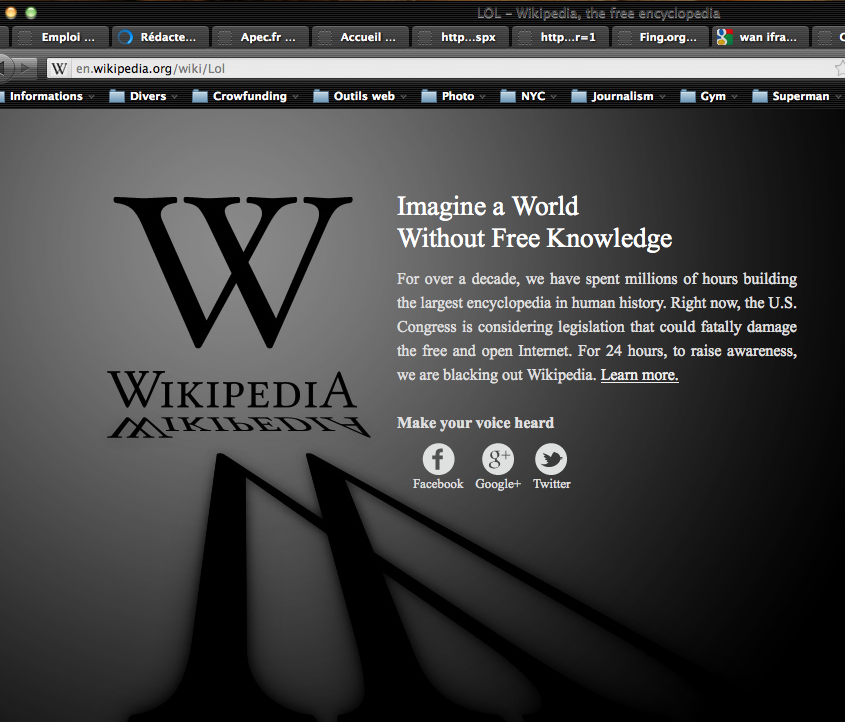
\includegraphics[height=\thumbheight]{sopa/looseduplicate9.png}
    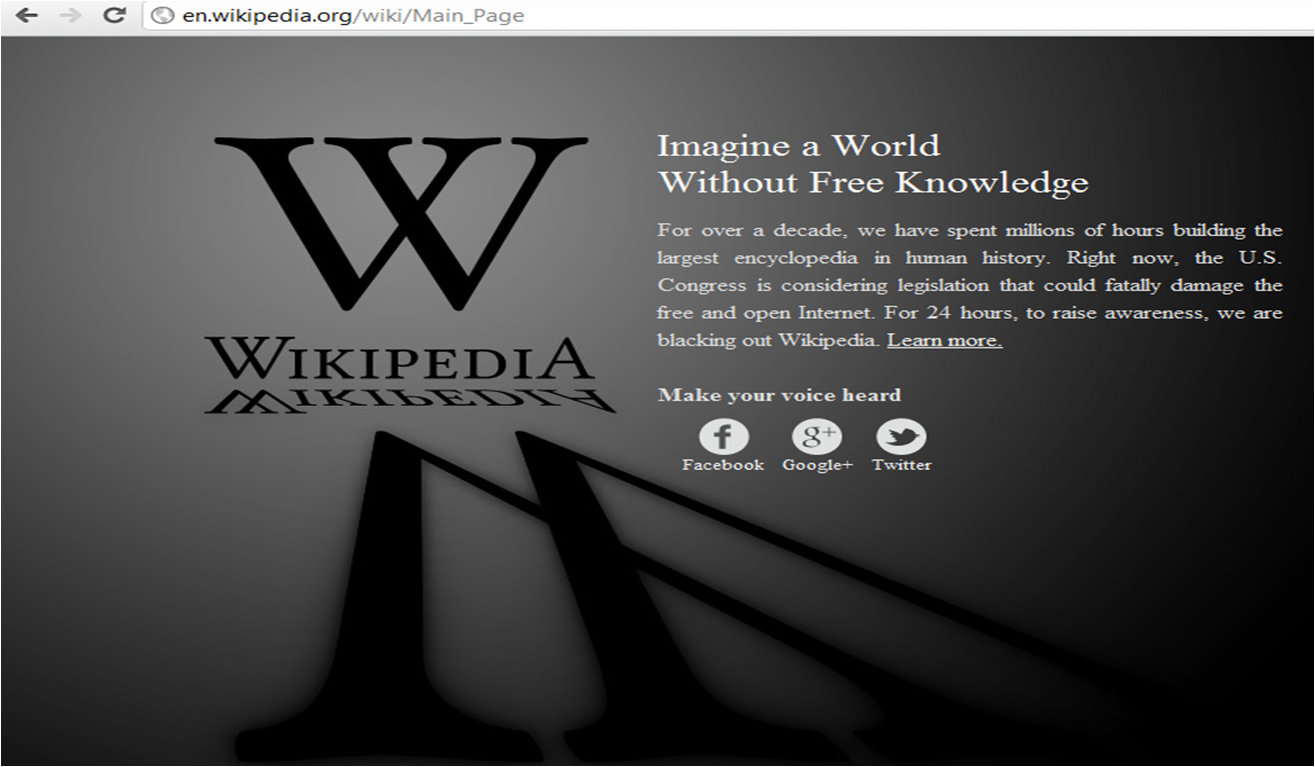
\includegraphics[height=\thumbheight]{sopa/looseduplicate10.png}
    
\includegraphics[height=\thumbheight]{sopa/looseduplicate11.jpg}
    
\includegraphics[height=\thumbheight]{sopa/looseduplicate12.jpg}
  \end{thumbsequence}
  \begin{thumbsequence}
    \setlength\fboxsep{0pt}
    \setlength\fboxrule{0.1mm}
    \fbox{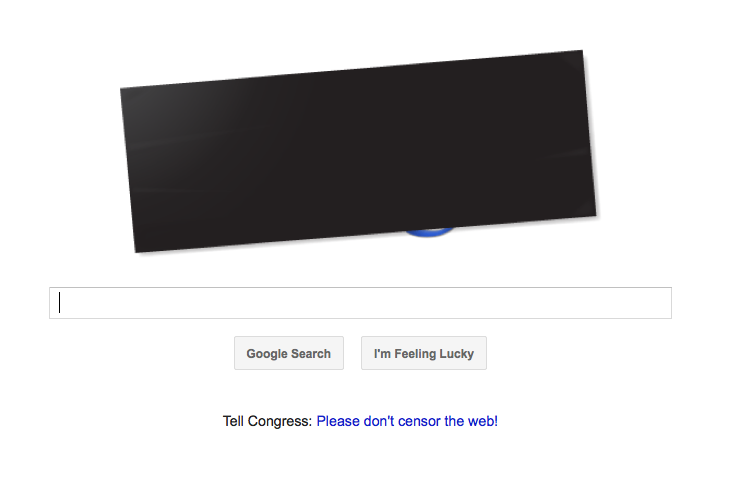
\includegraphics[height=\thumbheight]{sopa/looseduplicate13.png}}
    \fbox{
\includegraphics[height=\thumbheight]{sopa/looseduplicate14.jpg}}
\end{thumbsequence}
\end{tabular}

\begin{tabular}{p{\textwidth}}
\eventtitle{Christian Wulff Case}
  \begin{thumbsequence}
    \doublebox{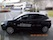
\includegraphics[height=\thumbheight]{wulff/exactduplicate1.jpg}}
    \doublebox{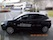
\includegraphics[height=\thumbheight]{wulff/exactduplicate2.jpg}}
  \end{thumbsequence}
  \begin{thumbsequence}
    \doublebox{
\includegraphics[height=\thumbheight]{wulff/exactduplicate3.jpg}}
    \doublebox{
\includegraphics[height=\thumbheight]{wulff/exactduplicate4.jpg}}
  \end{thumbsequence}
\end{tabular}

\begin{tabular}{p{\textwidth}}
\eventtitle{Free Mobile Launch}
  \begin{thumbsequence}
    \doublebox{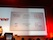
\includegraphics[height=\thumbheight]{free/exactduplicate1.jpg}}
    \doublebox{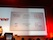
\includegraphics[height=\thumbheight]{free/exactduplicate2.jpg}}
  \end{thumbsequence}
  \begin{thumbsequence}
    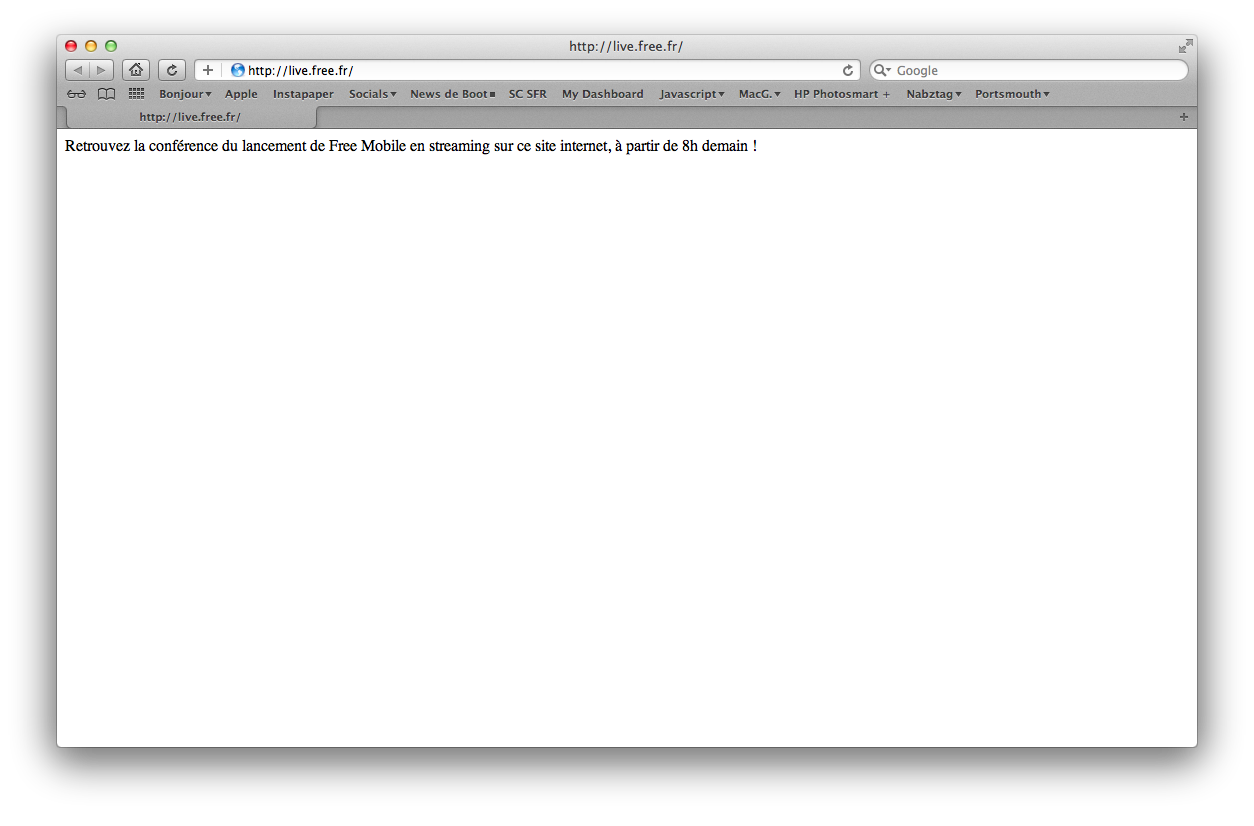
\includegraphics[height=\thumbheight]{free/looseduplicate1.png}
    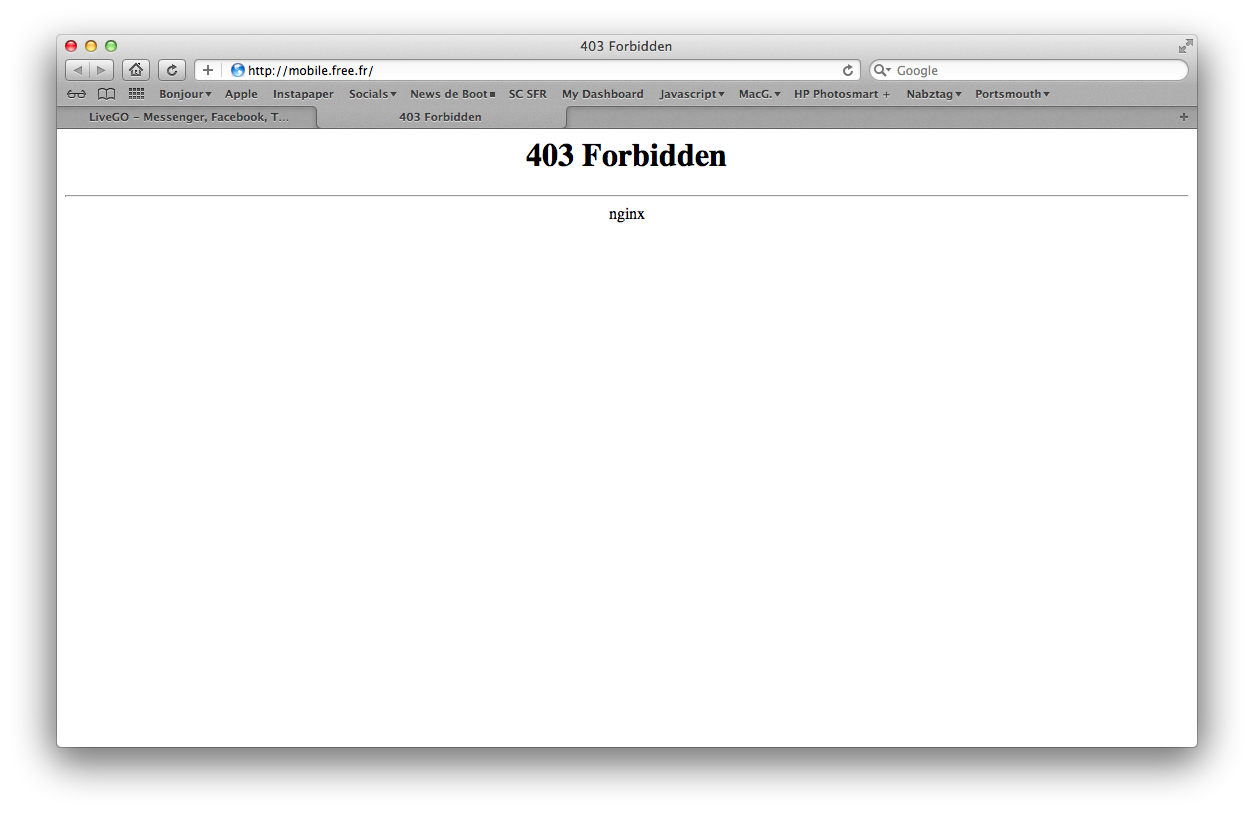
\includegraphics[height=\thumbheight]{free/looseduplicate2.png}
  \end{thumbsequence}
  \begin{thumbsequence}
    
\includegraphics[height=\thumbheight]{free/looseduplicate7.jpg}
    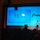
\includegraphics[height=\thumbheight]{free/looseduplicate8.jpg}
  \end{thumbsequence}
  \\[4pt]
  \begin{thumbsequence}
    
\includegraphics[height=\thumbheight]{free/looseduplicate15.jpg}
    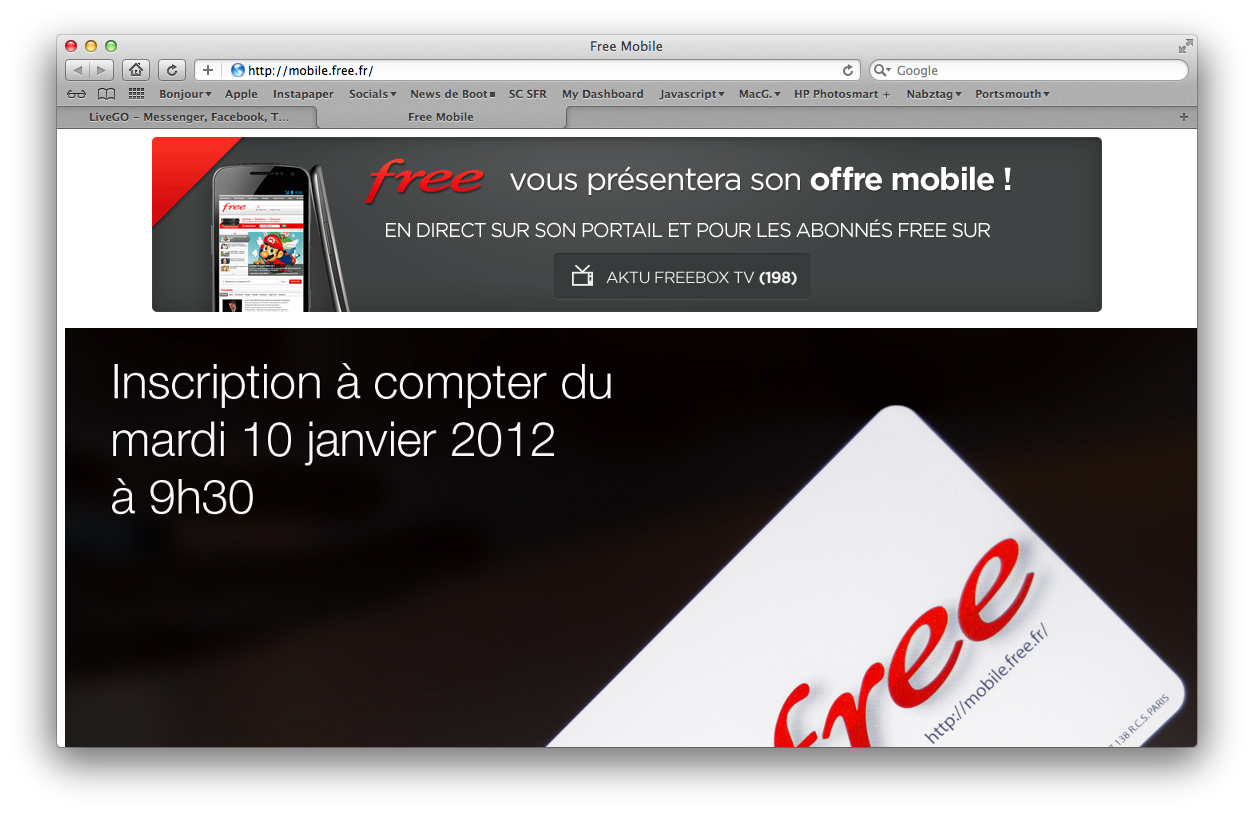
\includegraphics[height=\thumbheight]{free/looseduplicate16.png}
  \end{thumbsequence}
  \begin{thumbsequence}
    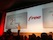
\includegraphics[height=\thumbheight]{free/looseduplicate9.jpg}
    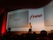
\includegraphics[height=\thumbheight]{free/looseduplicate10.jpg}
    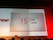
\includegraphics[height=\thumbheight]{free/looseduplicate11.jpg}
  \end{thumbsequence}
  \begin{thumbsequence}
    
\includegraphics[height=\thumbheight]{free/looseduplicate3.jpg}
    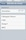
\includegraphics[height=\thumbheight]{free/looseduplicate4.jpg}
  \end{thumbsequence}
  \newstrip
  \begin{thumbsequence}
    
\includegraphics[height=\thumbheight]{free/looseduplicate12.jpg}
    
\includegraphics[height=\thumbheight]{free/looseduplicate13.jpg}
    \includegraphics[height=\thumbheight]{free/looseduplicate14.jpg}
  \end{thumbsequence}
  \begin{thumbsequence}
    \includegraphics[height=\thumbheight]{free/looseduplicate5.jpg}
    \includegraphics[height=\thumbheight]{free/looseduplicate6.jpg}
  \end{thumbsequence}
\end{tabular}

\begin{tabular}{p{\textwidth}}
\eventtitle{Costa Concordia Disaster}
  \begin{thumbsequence}
    \includegraphics[height=\thumbheight]{concordia/looseduplicate1.jpg}
    \includegraphics[height=\thumbheight]{concordia/looseduplicate2.jpg}
  \end{thumbsequence}
  \begin{thumbsequence}
    \includegraphics[height=\thumbheight]{concordia/looseduplicate3.jpg}
    \includegraphics[height=\thumbheight]{concordia/looseduplicate4.jpg}
  \end{thumbsequence}
  \begin{thumbsequence}
    \includegraphics[height=\thumbheight]{concordia/looseduplicate5.jpg}
    \includegraphics[height=\thumbheight]{concordia/looseduplicate6.jpg}
  \end{thumbsequence}
\end{tabular}

\begin{tabular}{p{\textwidth}}
\eventtitle{CES Las Vegas}
  \begin{thumbsequence}
    \includegraphics[height=\thumbheight]{ces/looseduplicate1.jpg}
    \includegraphics[height=\thumbheight]{ces/looseduplicate2.jpg}
    \includegraphics[height=\thumbheight]{ces/looseduplicate3.jpg}
    \includegraphics[height=\thumbheight]{ces/looseduplicate4.jpg}
    \includegraphics[height=\thumbheight]{ces/looseduplicate5.jpg}
  \end{thumbsequence}
  \begin{thumbsequence}
    \includegraphics[height=\thumbheight]{ces/looseduplicate6.jpg}
    \includegraphics[height=\thumbheight]{ces/looseduplicate7.jpg}
  \end{thumbsequence}
  \begin{thumbsequence}
    \includegraphics[height=\thumbheight]{ces/looseduplicate8.jpg}
  \end{thumbsequence}
\end{tabular}
\caption[Sample photos for some of the considered nine events]
  {Sample photos for some of the considered nine events
         (showing only exact- or near-duplicate media items)}
\label{fig:sequences}
\end{figure*}


\subsection{The Need for Media Item Deduplication}
\label{sec:the-need-for-media-item-deduplication}

Given our broad approach to retrieve media items
across multiple social networks,
we observed many exact-duplicate or near-duplicate media items.
Oftentimes, these duplicates stem from users who
cross-post to several social networks.
Instead of trying to filter out cross-posted items,
we rather keep them and cluster them.
We are especially interested in social interactions
that media items can trigger.
For example, if one and the same photo
is cross-posted to separate networks,
it can retrieve shares, likes, views, or comments
independently on each of those networks.
By clustering media items, we get a~higher-level view on
a~media item cluster's overall performance on different networks.
We also observed media items that were near-duplicates,
for example, from people who attended the same event like a~concert
and who took photos of the stage from almost the same angle.
Similar to exact-duplicates,
by clustering near-duplicate media items,
we can treat them like exact-duplicates to get the same
network-agnostic viewpoint.
We will examine reasons for exact-duplicate and near-duplicate
media item content and ways to deal with it in \autoref{cha:media-item-deduplication}.

\subsection{The Need for Ranking Media Items}

Our ultimate goal is to generate media galleries
that \emph{visually} and \emph{audially} summarize events.
Especially given high-recall search terms,
we need a~way to rank and prune media items.
Popular media items can be displayed bigger, longer,
or with a~special decoration like a~thicker border
in comparison to less popular media items.
For videos, the audio part poses a~challenge.
In our experiments, we observe that intermixing the audio
of all videos of an event often generates
a very characteristic \emph{noise cloud}
that \emph{audially} conveys the event's atmosphere very well.
A~good example is the Assad Speech event,
where a~mix of Arabic voices blends nicely
with the speech of a~US politician.
A~different example is the CES Las Vegas event,
where the atmosphere of a~big exposition with music,
announcements, and technical analysis becomes alive.
We will have a~closer look at media item ranking in
\autoref{cha:media-item-ranking}.

\section{Conclusions}

In this chapter, we have presented a~generic media extractor
for extracting media items shared on social networks to
illustrate known events.
We have proposed a~common abstraction layer on top of the
social networks' native data formats to align search results.
Our approach to extracting media items and associated
textual microposts covers already most of
the Western world's social networks.
Context-aware multimedia analysis will bring a~new range of
parameters into play since many media items contain a~message
that is complementary to the text.
For example, facial detection~\cite{viola2004facedetection}
and eventually recognition~\cite{wright2009facerecognition}
can signify the presence of specific people in a~media item.
Optical Character Recognition (OCR) can generate
additional textual signals from media items.
As visual recognition systems grow more powerful,
more objects will eventually be recognizable by
machines~\cite{serre2007objectrecognition},
which would allow for generating \emph{visual hashtags}
that describe the content
\emph{inside} of the media item.
Extracted features in all three categories
(\emph{textual}---from the micropost,
\emph{visual}---from the media item,
and \emph{social}---from the social network
in the form of social interactions)
can serve as ranking criteria, be it in isolation
or in combination by introducing a~ranking formula.
As a~result, this will also positively influence
the diversity of automated summarizations.

Nonetheless, it remains important to view the media and the
accompanying microposts as a~whole, since the text
could convey a~sentiment about,
or an explanation of the visual data.
Using named entity recognition as outlined in
\autoref{cha:micropost-annotation},
the important semantic elements in the micropost get identified.
The content of the message can subsequently be used
to narrow down the search space for visual factors
enabling cross-fertilization between the textual
and visual analysis, which results in effective context-aware analysis possibilities~\cite{verborgh2012multimediaannotation,rizzo2012whatfresh}.
Finally, by leveraging the \emph{LOD} cloud,
we can use that knowledge to get a~more diverse view on events.
At time of writing, the so-called
\emph{Operation Pillar of
Defense\footnote{\url{http://en.wikipedia.org/wiki/Operation_Pillar_of_Defense}, accessed July 15, 2013}}
by the Israeli armed forces
causes ongoing conflicts between Palestinians and Israelis.
Using the LOD cloud, promising search terms like, for example,
\emph{gaza}, can be easily looked up in different languages
like Hebrew or Arabic.
In practice, these additional search terms return interesting
new media items that a~pure monolingual search
would not have revealed---oftentimes,
and especially in the concrete case,
at the expense of neutrality.
We are confident that the additional coverage
from more angles helps sharpen one's own viewpoint of an event,
especially with the option of translating microposts
authored in foreign languages%
---which is supported by our approach---%
as mentioned in \autoref{sec:machine-translation}.

\section*{Chapter Notes}
This chapter is partly based on the following publications.
%\cite{rizzo2012whatfresh,khrouf2012aggregatingsocialmedia,khrouf2012confomaton}.

\begin{itemize}
  \item \onlyfullcite{rizzo2012whatfresh}.
  \item \onlyfullcite{khrouf2012aggregatingsocialmedia}.
  \item \onlyfullcite{khrouf2012confomaton}.
\end{itemize}

\clearpage
\printbibliography[heading=subbibliography]
\chapter{Media Item Deduplication}
\label{sec:media-item-deduplication}

% the code below specifies where the figures are stored
\ifpdf
    \graphicspath{{6_media_item_deduplication/figures/PNG/}{6_media_item_deduplication/figures/PDF/}{6_media_item_deduplication/figures/}}
\else
    \graphicspath{{6_media_item_deduplication/figures/EPS/}{6_media_item_deduplication/figures/}}
\fi

\section{Introduction}

In the previous \autoref{cha:media-item-extraction}
in \autoref{sec:the-need-for-media-item-deduplication},
we have motivated the need for media item deduplication.
By clustering media items, we get a~higher level view on
a~media item cluster's overall performance on different networks.
As detailed in \autoref{sec:definition}, media items can be
photos or videos.
WordNet~\cite{fellbaum1998wordnet,miller1995wordnet} defines
the term \emph{duplicate} as
\textit{``a copy that corresponds to an original exactly''}.
the corresponding verb \emph{to duplicate} is defined as to
\textit{``make a~duplicate or duplicates of''}.
The derived term \emph{deduplication} in consequence refers to
the act of eliminating duplicate or redundant information.

\subsection{Definition of Exact Duplicate for Photos}

We define two media items of type photo as \emph{exact duplicate},
if their pixel contents are exactly the same.
This implies that by our definition, a~scaled version
of the same photo is \emph{not} an exact duplicate. 
Similarly, a~rotated version of a~photo is also \emph{not}
an exact duplicate. 
In contrast, two photo files with different file names,
or different Exchangeable image file
format\footnote{\url{http://www.cipa.jp/english/hyoujunka/kikaku/pdf/DC-008-2010_E.pdf},
accessed November 22, 2012}
(Exif) data, are considered exact duplicate,
if their pixel contents are exactly the same.
Exact duplicate photos typically occur if users share content 
from one social network on another, for example,
if one user posts a~photo on Instagram that then someone else
(or even the same user) posts on Facebook.

\subsection{Definition of Near-Duplicate for Photos}

We define two media items of type photo as \emph{near-duplicate},
if their pixel contents differ no more than a~given threshold.
Examples of near-duplicate photos are scaled versions
of the same photo, photos shot from a~slightly different angle,
rotated photos up to a~certain degree, \emph{etc.}
Near-duplicate photos typically occur if event attendants
stand close to each other and thus take photos
from a~similar standpoint.
Another scenario is a~user applying a~photo effect to a~photo
(like an Instagram filter) and then sharing both, the modified,
and the unmodified version.

\subsection{Definition of Exact Duplicate for Videos}

We define two media items of type video as \emph{exact duplicate},
if their pixel contents are frame by frame exactly the same.
In practice, we lower this condition and instead of every frame
only consider frames at shot boundaries.
We make \emph{no} requirements on the audio, \emph{i.e.},
a video in two different languages, however, that fulfills the 
pixel contents equality condition, is considered exact duplicate.
Typical scenarios where exact duplicate videos can occur is,
for example, two users sharing the same YouTube video
independently from each other.

\subsection{Definition of Near-Duplicate for Videos}

We define two media items of type video as \emph{near-duplicate},
if their pixel contents per frame differ no more
than a~given threshold.
In practice, we lower this condition and instead of every frame
only consider frames at shot boundaries.
Typical scenarios where near-duplicate videos can occur is through
logo or subtitle insertion, resizing, re-encoding,
or aspect-ration changes.
Note, we do not consider video subsegments near-duplicates.

\subsection{Special Case of Photo Contained in a~Video}

We define the special case of
\emph{a photo being contained in a~video} if the pixel contents
of a~photo media item differ no more than a~given threshold from
the pixel contents of any of the frames of a~video media item.
In practice, we lower this condition and instead of every frame
only consider frames at shot boundaries.
Typically, this phenomenon occurs if two event attendants
of the same event both cover the event from almost the same
standpoint, however, if the one attendant takes a~video,
while the other attendant takes a~photo.

\subsection{Motivation and Chapter Outline}

In this chapter, we will treat video
and photo deduplication separately. 
Our goal is to deduplicate media items on-the-fly
at the very moment they are extracted from social networks.
Due to this limitation, we cannot rely on any preprocessing
at all that state-of-the-art algorithms rely on.
This is why we dedicate a~whole section entirely to on-the-fly
shot boundary detection for online video,
which is by no means a~solved problem.
The contribution of our approach is that it is entirely Web-based
and on-the-fly, which introduces interesting new challenges
that traditional approaches to shot boundary detection
do not have to cope with.
Our Web-based approach abstracts away most of the low-level details
like the video codec, in favor of the high-level \texttt{<video>}
API, however, this also comes at a~cost.
A~major issue is the uncertain streaming speed,
where traditional approaches have immediate access
to the video file on disk.
An additional challenge is the unknown key frame distribution
of the target videos, which---together with streaming speed
issues---makes exact frame-wise video navigation impossible.
Our approaches to video and photo near-duplicate
and exact duplicate detection are founded
on a~tile-wise histogram-based pixel comparison algorithm.

\section{Video Shot Boundary Detection}
Video shot boundary detection is the processor-intensive task
of splitting a~video into continuous camera shots,
with hard or soft cuts as the boundaries.
In this section, we present a~browser-based, client-side, and
on-the-fly approach to this challenge
based on modern HTML5~\cite{berjon2012html5} Web APIs.
Once a~video has been split into shots,
shot-based video navigation gets enabled,
more fine-grained playing statistics can be created,
and finally, shot-based video comparison is possible.
\autoref{fig:screenshot} shows detected camera
shots for a~sample video.
The algorithm has been incorporated in a~browser extension
such that it can run transparently on a~major online video portal.

\begin{figure}
  \begin{center}
    \includegraphics[width=0.7\linewidth]{./stevejobs.png}
  \end{center}
  \caption{Camera shots for a~sample video on 
    a~major online video portal, detected on-the-fly via
    our shot boundary algorithm incorporated
    in a~browser extension.}
  \label{fig:screenshot}
\end{figure}

\subsection{Related Work} \label{sec:related-work}
Video fragments consist of shots, which are sequences of
consecutive frames from a~single viewpoint,
representing a~continuous action in time and space.
The topic of shot boundary detection has already been described
extensively in literature.
While some specific issues still remain
(notably gradual transitions and false positives
due to large movement or illumination changes),
the problem is considered resolved for many
cases~\cite{yuan2007shotboundary,hanjalic2002shotboundary}.
Below, we present an overview of several well-known categories of shot boundary detection techniques.

\emph{Pixel comparison
methods}~\cite{hampapur1994videosegmentation,
zhang1993videopartitioning} construct a~discontinuity metric
based on differences in color or intensity values
of corresponding pixels in successive frames.
This dependency on spatial location makes this technique
very sensitive to (even global) motion.
Various improvements have been suggested, such as prefiltering
frames~\cite{zhang1995videoparsing},
but pixel-by-pixel comparison methods proved inferior in the end
and have steered research towards other directions.

A~related method is
\emph{histogram analysis}~\cite{otoole1999shotboundary},
where changes in frame histograms are used
to justify shot boundaries.
Their insensitivity to spatial information
within a~frame makes histograms less prone to partial
and global movements in a~shot.

As a~compromise, a~third group of methods consists of
a~\emph{trade-off between the above two
techniques}~\cite{ahmed1999keyframe}.
Different histograms of several, non-overlapping blocks
are calculated for each frame,
thereby categorizing different regions of the frame
with their own color-based, space-invariant fingerprint.
The results are promising, while computational complexity
is kept to a~minimum, which is why we have chosen
a~variation of this approach for our own algorithm.

Other approaches to shot boundary detection include
the \emph{comparison of mean and standard deviations}
of frame intensities~\cite{lienhart1999comparison}.
Detection using other features such as
edges~\cite{zabih1995scenebreaks} and
motion~\cite{bouthemy1997shotchange} have also been proposed.
However, Gargi \emph{et~al.} have shown that
these more complex methods do not necessarily
outperform histogram-based approaches~\cite{gargi2000videoshot}.
A~detailed comparison can be found in
Yuan~\emph{et~al.}~\cite{yuan2007shotboundary}.

\subsection{Shot Boundary Detection Algorithm}
\label{sec:details-of-algo}

In this section, we discuss our shot boundary detection algorithm,
which falls in the category of histogram-based algorithms.
Since visually dissimilar video frames
can have similar global histograms,
instead we take local histograms into account. 
We therefore split video frames in freely configurable
rows and columns, \emph{i.e.}, lay a~grid of tiles over each frame.
The user interface, as can be seen in \autoref{fig:algorithm},
currently allows for anything from a~$\mathit{1} \times \mathit{1}$ 
grid to a~$\mathit{20} \times \mathit{20}$ grid.
For each step, we examine a~frame $\mathit{f}$ and its direct
predecessor frame $\mathit{f - 1}$.

Apart from the per-tile average histogram distance,
the frame distance function further considers
a~freely configurable number of \emph{most different} and
\emph{most similar} tiles.
This is driven by the observation that different parts
of a~video have different intensities of color changes,
dependent on the movements from frame to frame.
The idea is thus to boost the influence of movements in the frame
distance function, and to limit the influence of permanence.
In the debug view of our approach, as depicted in
\autoref{fig:algorithm}, blue boxes indicate movements,
while red boxes indicate permanence.
In the concrete example, Steve Jobs' head and shoulders move
as he talks, which can be clearly seen
at the blue boxes in the particular tiles.
Additional movements come from a~swaying flag on the left,
and a~plant on the right.
In contrast, the speaker desk, the white background,
and the upper part of his body remain static,
resulting in red boxes.
For this example, we use a~grid layout of
$\mathit{20} \times \mathit{20}$ tiles
($\mathit{nTiles} = \mathit{400}$),
and an empirically determined  number
$\mathit{tileLimit}$ of most different or similar tiles,
\emph{i.e.}, we treat one third of all tiles
as most different tiles, one third as normal tiles,
and one third as most similar tiles,
and apply boosting and limiting factors to the most different
and most similar tiles respectively.
We work with values of~$\mathit{1.1}$ for the
$\mathit{boostingFactor}$, which slightly increases
the impact of the most different tiles,
and $\mathit{0.9}$ for the $\mathit{limitingFactor}$,
which slightly decreases the impact of the most similar tiles.
The algorithm pseudo code can be seen in \autoref{code:algorithm}.

We define the average histogram distance between two frames
$\mathit{f}$ and $\mathit{f - 1}$ as $\mathit{avgHisto}_{f}$.
In a~first step, we have examined the histogram distance
data statistically, and observed that while
the overall average frame distance $\mathit{avgDist}_{f}$,
defined as $$\mathit{avgDist}_{f} =
\frac{1}{\mathit{nTiles}}\sum_{t=1}^{\mathit{nTiles}}
\mathit{avgHisto}_{f, t}$$ is very intuitive to human beings,
far more value lies in the standard deviation
$\mathit{stdDev}_{f}$, based on the definition of the overall
average frame distance $\mathit{avgDist}_{f}$
$$\mathit{stdDev}_{f} =
\sqrt{\frac{1}{\mathit{nTiles}}\sum_{t=1}^{\mathit{nTiles}}
(\mathit{avgHisto}_{f, t} - \mathit{avgDist}_{f})^{2}}$$
We use the standard deviation as a~value for the shot splitting
threshold~\cite{lienhart1999comparison}
to come to very accurate shot splitting results.
We found the boosting and limiting factors to have an overall
positive quality impact on more lively videos,
and a~negative quality impact on more monotone videos.
Best results can be achieved if,
after changing either the boosting or the limiting factors
for the most similar or different tiles,
the value of the shot splitting threshold is adapted
to the new resulting standard deviation.
The user interface optionally does this automatically.

\begin{figure}
  \begin{center}
    \includegraphics[width=1.0\linewidth]{./algorithm.png}
  \end{center}
  \caption{Debug view of the shot boundary detection process.
    Blue boxes highlight tiles with the most differences
    to the previous frame, red boxes those with most similarities.}
  \label{fig:algorithm}
\end{figure}

\begin{lstlisting}[caption=Pseudocode of shot boundary detection
  algorithm.,
  label=code:algorithm, float]
for frame in frames
  f = frame.index  
  for tile in tiles of frame      
    avgHisto[f][tile] = getTilewiseDiff()
 
  mostDiffTiles = getMostDiffTiles(avgHisto[f])
  mostSimTiles = getMostSimTiles(avgHisto[f])
 
  for tile in tiles of frame    
    factor = 1  
    if tile in mostDiffTiles
      factor = boostingFactor
    else if tile in mostSimTiles
      factor = limitingFactor
    avgHisto[f][tile] = avgHisto[f][tile] * factor
  avgDist[f] = avg(avgHisto[f])
\end{lstlisting}

\subsection{Implementation Details}
\label{sec:implementation}

The complete video analysis process happens fully
on the client side.
We use HTML5 JavaScript APIs of the \texttt{<video>} and
\texttt{<canvas>} tags.
In order to obtain a~video still frame
from the \texttt{<video>} tag at the current video position,
we use the \texttt{drawImage()} function of the 2D context of the
\texttt{<canvas>} tag,
which as its first parameter accepts a~video.
We then analyze the video frame's pixels tile-wise
and calculate the histograms.
In order to retrieve the tile-wise pixel data
from the 2D context of the \texttt{<canvas>},
we use the \texttt{getImageData()} function.
For processing speed reasons, we currently limit our approach to
a~resolution of one second, \emph{i.e.},
for each analysis step,
seek the video in $\mathit{1s}$ steps.
We then calculate the frame distances as outlined in
\autoref{sec:details-of-algo}.
For each frame, we can optionally generate an \texttt{<img>} tag
with a~base64-encoded data URI representation
of the video frame's data
that can serve for filmstrip representations of the video.

\subsection{Evaluation} \label{sec:evaluation}

Detecting shots on-the-fly in streaming video
comes with its very own challenges.
First, it is a~question of streaming speed.
Especially with high-definition (HD) video,
this can be very demanding.
We do not attach the analysis \texttt{<video>} tag
to the DOM tree~\cite{lehors2004dom} to save some CPU cycles,
however, the video still needs to be sought to each frame
in one second-steps and be processed.
Even on a~higher-end computer (our experiments ran on a~MacBook
Pro, Intel Core 2 Duo 2,66 GHz, 8 GB RAM),
the process of analyzing and displaying in parallel
a~$\mathit{1280} \times \mathit{720}$ HD video of media type
\emph{video/mp4; codecs="avc1.64001F, mp4a.40.2"}
caused an average CPU load of about 70\%.
The HTML5~\cite{berjon2012html5} specification states that
\textit{``when the playback rate is not exactly 1.0,
hardware, software, or format limitations can cause video frames
to be dropped''}.
In practice, this causes the analysis environment
to be far from optimal.
In our experiments we differentiated between false positives,
\emph{i.e.}, shot changes that were detected,
but not existent, and misses, \emph{i.e.},
shot changes that were existent,
but not detected.
Compared to a~set of videos with manually annotated shot changes,
our algorithm detected fewer false positives than misses.
The reasons were gradual transitions and shots
shorter than one second (below our detection resolution)
for misses, and large movements in several tiles
for false positives.
Overall, we reached an accuracy of about 86\%,
which is not optimal, but given the challenges
sufficient for our use case of
detecting near- or exact duplicate videos. 

\subsection{Optimization Potential}

Optimization potential lies in
improving the analysis speed by dynamically selecting
lower quality analysis video files,
given that videos are oftentimes available in several resolutions
(both LD and HD).
We will check in how far analysis results differ
for the various qualities.
Second, more advanced heuristics for the various user-definable
options in the analysis process are needed.
While there is no optimal configuration for all types of videos,
there are some key indicators that can help categorize videos
into classes and propose predefined known working settings
based on the standard deviation $\mathit{stdDev_{f}}$
and the overall average frame distance $\mathit{avgDist_{f}}$.
Both are dependent on the values of $\mathit{boostingFactor}$,
$\mathit{limitingFactor}$, $\mathit{rows}$, and $\mathit{columns}$. 
Interpreting our results so far, there is evidence
that low complexity settings are sufficient in most cases,
\emph{i.e.}, a~number of $\mathit{rows}$ and $\mathit{columns}$
higher than~$\mathit{2}$ does not necessarily
lead to more accurate shot boundary detection results.
The same applies to the number of to-be-considered most different
or similar tiles $\mathit{tileLimit}$.
We had cases where not treating those tiles differently
at all, \emph{i.e.}, setting
$\mathit{boostingFactor} = \mathit{limitingFactor} = \mathit{1}$, 
led to better results.

\section{Photo Deduplication}

We determine the popularity of media items shared across
social networks.
This task involves the deduplication of extracted media items.
In the previous section, we have presented an algorithm
for on-the-fly shot boundary detection for video media items.
In this section, we will show how components of this algorithm
can be used to deduplicate images.
First, we look at related work for the task of photo deduplication.

\subsection{Related Work}

Work on ordinal measures that serve as a~general tool for
image matching was performed by Bhat \emph{et al.}\
in~\cite{bhat1998imagecorrespondence}.
Chum \emph{et al.}\ have proposed a~near-duplicate image detection method using min-Hash and
term frequency--inverse document frequency (tf--idf)
weighting~\cite{chum2008nearduplicate}.
The proposed method uses a~visual vocabulary of vector quantized local feature descriptors based on
Scale Invariant Feature Transform (SIFT)~\cite{lowe1999sift}.
A~method for both photos and video~\cite{yang2009nearduplicate}
has been proposed by Yang \emph{et al.}

\subsection{Experiments}

\subsection{Evaluation}

\section{Video Deduplication}

\subsection{Related Work}

In addition to the before-mentioned  combined approach
for video and photo near-duplicate
detection~\cite{yang2009nearduplicate}, also more
specialized methods for video deduplication exist,
for example~\cite{min2011nearduplicatevideo,wu2009nearduplicate},
by Min \emph{et al.}\ who, given the observation that 
transformations tend to preserve the semantic information conveyed
by the video content, propose a novel approach for identifying
near-duplicate videos by making use of both low-level visual
features and high-level semantic features
detected using trained classifiers.
Further, there is~\cite{oliveira2010nearduplicate} by Oliveira
\emph{et al.}\ who look at near-duplicate video detection
from a human angle.  
The authors have conducted four large-scale surveys
and have confirmed that humans perceive videos as near-duplicates
both based on non-semantic features like different image or audio
quality, but also based on semantic features like different
videos of similar content, where, according to the authors,
most research still focuses mostly on the non-semantic features.
A~survey of video deduplication methods has been conducted by
Lian \emph{et al.}\ in~\cite{lian2010survey}.

\subsection{Experiments}

\subsection{Evaluation}

\section{Conclusion}

\section*{Chapter Notes}
This chapter is partly based on the following publications:
\todo{Add publications}
\chapter{Media Item Ranking}
\label{sec:media-item-ranking}

% the code below specifies where the figures are stored
\ifpdf
    \graphicspath{{7_media_item_ranking/figures/PNG/}{7_media_item_ranking/figures/PDF/}{7_media_item_ranking/figures/}}
\else
    \graphicspath{{7_media_item_ranking/figures/EPS/}{7_media_item_ranking/figures/}}
\fi

\section{Introduction}

In the previous chapter, we have motivated and shown methods
to deduplicate exact duplicate and near-duplicate media items.
In this chapter, we introduce ranking criteria and methods
to put deduplicated media clusters in a~well-defined order.
The application screenshots that can be seen in \autoref{fig:topvsfashionshow}
and \autoref{fig:topgrammy} show the---besides publication time (or recency)---%
most intuitive ranking criterion one can imagine:
ranking by occurrence popularity.
The more often a~media item (or a~near-duplicate of it)
appears in any of the considered social networks, 
the higher it should be ranked.
However, ranking by occurrence popularity (or media item cluster size)
disregards one of the most valuable features of social networks: 
the social aspects.
In consequence, in this chapter, we will introduce
further media item ranking criteria that,
together with media item cluster size,
will allow us to come up with more adequate social media item ranking mechanisms.

\section{Evaluating Subjective Data}

Evaluating subjective data, like \emph{the} correct ranking
for a~set of media items, is a~challenging task.
For different users, there may be different optimal settings.
A~common subjective evaluation technique
is the Mean~Opinion Score (MOS)~\cite{itu1998mos}.
Traditionally, MOS is used for conducting subjective evaluations
of telephony network transmission quality,
however, more recently, MOS has also found
wider usage in the multimedia community
for evaluating \emph{per se} subjective things
like perceived quality from the users' perspective. 
Therefore, a~set of standard, subjective tests are conducted,
where a~number of users rate the quality of test samples
with scores ranging from 1 (worst) to 5 (best).
The actual MOS is then the arithmetic mean of all individual scores.
Given a~subjective evaluation criterion
like the correctness of a~ranking,
MOS provides a~meaningful way to judge the overall quality of our approach.

\section{Media Item Ranking Criteria}

In this section, we describe several criteria that can serve to rank
media items retrieved from social networks. 
We base these criteria on the information available from
the media item extractors described in \autoref{cha:media-item-extraction},
which given event-related search terms
extract raw binary media items and associated microposts
from multiple social networks.

\subsection{Visual Ranking Criteria} \label{sec:visualrankingcriteria}

This category regards the contents of photos and videos.
We distinguish \emph{low-} and \emph{high-level} visual ranking criteria.
High-level criteria are, \emph{e.g.}, logo detection,
face recognition, and camera shot separation.
Low-level criteria are, \emph{e.g.}, file size, resolution,
duration of a~video, geolocation, and time.
Via OCR, contained characters can be treated as a~textual features.

\subsection{Audial Ranking Criteria}

This category regards the audio track of videos.
\emph{High-level} ranking criteria are the presence or absence
of silence, music, speech, or a~mixture thereof.
Similar to visual features before,
audial \emph{low-level} features are the average bit rate,
volume, possibly distorted areas, \emph{etc}.
Through audio-transcription, speech can be treated as a~textual feature.

\subsection{Textual Ranking Criteria}

This category regards the microposts that accompany media items.
Typically, microposts provide a~description of media items.
Using named-entity disambiguation tools,
textual content can be linked to LOD cloud concepts~\cite{Facebook2011}.
We have described micropost annotation in detail in \autoref{cha:micropost-annotation}.

\subsection{Social Ranking Criteria}

This category regards social network effects like shares, mentions,
view counts, expressions of (dis)likes, user diversity, \emph{etc}.
Prior work~\cite{khrouf2012aggregatingsocialmedia}
allows us to not only examine these effects
on a~\emph{single} social network,
but in a~\emph{network-agnostic} way across multiple social networks.
We will detail social aspects more later on in this chapter.

\subsection{Aesthetic Ranking Criteria}

This category regards the desired outcome after the ranking, \emph{i.e.},
the media gallery that illustrates a~given event and its atmosphere.
Studies exist for the aesthetics of
automatic photo book layout~\cite{sandhaus2011photobook},
photo aesthetics \emph{per se}~\cite{obrador2012photoaesthetics},
video and music playlist generation~\cite{knees2006musicplaylist,davidson2010videorecommendation},
however, to the best of our knowledge,
no media gallery composition aesthetics studies exist
that examine mixing video \emph{and} photo media items.

\subsection{Temporal Ranking Criteria}

This category regards the publication date of media items.
If media items are clustered, we use the youngest media item
as cluster representative.
Media items can be ranked by recency, as oftentimes more recent items
are more interesting in the streaming context of social networks.

\section{Social Interactions Abstraction Layer}
\label{sec:social-interactions-abstraction-layer}

As we have described in \autoref{cha:social-networks},
social networks have different paradigms of social interactions.
In \autoref{sec:data-format}, we have briefly presented the overall
abstraction layer on top of the native data formats
of all considered social networks in order to gain
an agnostic view on the underlying social networks.
In this section, we detail the part of the abstraction layer
that models the network-specific social interaction patterns.
Those interaction patterns must be exposed by the social network 
via specific API calls in order to be considered,
which only is the case for a~subset of the social networks we deal with.
In the subsections below, we have listed
how we abstract the social interactions in question on each social network.
In our concrete implementation, we differ unknown values
that are returned as \texttt{null}, \emph{i.e.},
where the information is not exposed,
from \texttt{0} values, where the value is known to be zero.
We briefly recall the social interactions part
of the abstraction layer's data format:

\begin{description}
  \item[\texttt{socialInteractions}] Container for social
    interactions
  \begin{description}  
  \item[\texttt{likes}] Number of times a~micropost was liked, or
    \texttt{null}
  \item[\texttt{shares}] Number of times a~micropost was shared, or
    \texttt{null}
  \item[\texttt{comments}] Number of comments a~micropost
    received, or \texttt{null}
  \item[\texttt{views}] Number of views a~micropost reached, or
    \texttt{null}
  \end{description}    
\end{description}

\subsection{Social Interaction ``Likes''}

We abstract the social interaction of liking a~media item
as instances of the following network-specific social interactions:

\begin{small_itemize}
  \item[] Facebook Like
  \item[] \googleplus \plusone
  \item[] Instagram Like
  \item[] Flickr Favorite
  \item[] YouTube Like, YouTube Favorite
  \item[] Twitter Favorite
\end{small_itemize}  

\subsection{Social Interaction ``Shares''}

We abstract the social interaction of resharing a~media item
as instances of the following network-specific social interactions:

\begin{small_itemize}
  \item[] Facebook Share
  \item[] \googleplus Share
  \item[] Twitter native ReTweet
\end{small_itemize}

\subsection{Social Interaction ``Comments''}

We abstract the social interaction of commenting on a~media item
as instances of the following network-specific social interactions:

\begin{small_itemize}
  \item[] Facebook Comments
  \item[] \googleplus Comments
  \item[] Instagram Comments
  \item[] Twitter manual, non-native ReTweet, @Replies
  \item[] Twitpic Comments
  \item[] MobyPicture Comments
  \item[] Flickr Comments
\end{small_itemize}

\subsection{Social Interaction ``Views''}

We abstract the social interaction of viewing a~media item
as instances of the following network-specific social interactions:

\begin{small_itemize}
  \item[] YouTube Views
  \item[] Flickr Views
  \item[] Twitpic Views
  \item[] Mobypicture Views
\end{small_itemize}

\section{Merging Social Interactions}
\label{sec:merging-social-interactions}

If a~set of media items is similar enough to be clustered
under the criteria that were detailed in
\autoref{cha:media-item-deduplication},
we can treat the whole of the cluster
as if it were just one media item.
Therefore, we need to specify a~merging strategy
for the associated data of the individual media items
in the particular cluster.
\autoref{code:merging} shows the pseudocode of the merging algorithm.
During the merging step,
we treat unknown values represented as \texttt{null} as \texttt{0}.
The algorithm accumulates individual social interactions
and assigns the accumulated social interactions to the cluster.

\begin{lstlisting}[caption=Pseudocode of the social interactions merging algorithm,
  label=code:merging, float]
for cluster in clusters
  likes = shares = views = comments = 0
  for mediaItem in cluster
    likes += mediaItem.likes ? mediaItem.likes : 0
    shares += mediaItem.shares ? mediaItem.shares : 0
    comments += mediaItem.comments ? mediaItem.comments : 0
    views += mediaItem.views ? mediaItem.views : 0
  end for
  cluster.socialInteractions.likes = likes
  cluster.socialInteractions.shares = shares
  cluster.socialInteractions.comments = comments
  cluster.socialInteractions.views = views
end for     
\end{lstlisting}

\section{Selection of a~Cluster's Visual Representative}  

As outlined in the previous section, similar enough media items
are clustered and treated as just one media item.
The previous section introduced
a~merging algorithm for the social interactions data.
In this section, we introduce an algorithm for the selection of
a~cluster's visual representative.
Naturally, through the way the clustering algorithm works,
the contained media items are already visually similar. 
In consequence, we fall back to using \emph{low-level}
visual ranking criteria as defined in \autoref{sec:visualrankingcriteria}.
\autoref{code:clusterrepresentative} shows the cluster representative
selection algorithm, which is based on the low-level feature \emph{resolution}.
The algorithm selects the media item with the highest megapixel resolution
as the cluster representative.

\begin{lstlisting}[caption=Pseudocode of the cluster representative selection algorithm,
  label=code:clusterrepresentative, float]
maxPixels = 0
clusterRepresentative = null
for mediaItem in cluster
  resolution = mediaItem.width * mediaItem.height
  if resolution >= maxPixels
    maxPixels = resolution
    clusterRepresentative = mediaItem
  end if  
end for
return clusterRepresentative     
\end{lstlisting}

\section{Ranking Media Item Clusters}

Up to now, we have shown how media item clusters are formed,
how each cluster's social interactions social interactions data is accumulated,
and how a~cluster's representative media item is selected.
In this section, we finally describe a~ranking formula to rank
a~set of media clusters that match a~given query.

In the ranking formula, we consider all the previously defined ranking criteria,
namely these are visual, audial, textual, temporal, social, and aesthetic.
For a~given set of media item clusters, a~ranking is calculated as follows.
$$ \alpha \times \mathit{likes} + \beta \times \mathit{shares} +
\gamma \times \mathit{comments} + \delta \times \mathit{views} +
\epsilon \times \mathit{crossNetwork} + \zeta \times \mathit{recency} $$
With the weight factors
$$ \alpha, \beta, \gamma, \delta, \epsilon, \zeta \in \mathbb{N} $$
The values $ \mathit{likes}, \mathit{shares}, \mathit{comments}, \mathit{views} $
stem from the individual media items as defined in \autoref{sec:data-format} and 
were accumulated as defined in \autoref{sec:merging-social-interactions}.
The value of $ \mathit{crossNetwork} $ corresponds to the length of the current cluster. 
Finally, the value of $ \mathit{recency} $ is calculated as follows.
If the youngest media item in the cluster is less than or exactly one day old, the value of
$ mathit{recency} $ is 8, for two days it is 4, for three days it is 2, and for each day more, the value is 1.

\section{Evaluation}

\subsection{Super Bowl Analyses by Social Networks}

We have evaluated our approach with the at time of writing
recent event of the Super Bowl XLVII%
\footnote{\url{http://en.wikipedia.org/wiki/Super_Bowl_XLVII},
accessed February 8, 2013}.
This event received broad social media coverage, and the social networks
Twitter\footnote{\url{http://blog.twitter.com/2013/02/the-super-tweets-of-sb47.html},
accessed February 8, 2013},
Instagram\footnote{\url{http://blog.instagram.com/post/42254883677/sbroundup},
accessed February 8, 2013}, and
Facebook\footnote{\url{http://newsroom.fb.com/News/570/Super-Bowl-XLVII-on-Facebook},
accessed February 8, 2013} all published blog posts with analyses of the event
on the respective networks,
whereas the search engine Google%
\footnote{\url{http://googleblog.blogspot.com/2013/02/m-beyonce-and-ravens-dominate-game-day.html},
accessed February 8, 2013}
published an analysis of trending queries during the match.
In the following, we provide summaries of these different analyses,
with the expectation to encounter relevant media items
for each of the mentioned highlights in the final ranked list of media items
stemming from the various social networks.

According to Twitter's analysis, the five moments that generated the most tweets
during the game (see the Wikipedia-provided game summary for details)
ordered by decreasing number of tweets per minute were
the power outage,
the 108-yard kickoff return for the Ravens touchdown by Jones,
the moment when the clock expired and the Ravens won,
Jones catches a~56 yard pass for a~Ravens touchdown,
and the Gore touchdown for the 49ers.
Overall, 24.1 million tweets about the game and halftime show were counted,
a~number that even leaves aside the advertisements.
The Twitter article further mentions the performance by superstar artist Beyoncé 
and a~number of Super Bowl advertisements as highlights of the event.   

Instagram's analysis mentions that more than three million photos
with Super Bowl-related words in their captions were shared and
at peak more than 450 photos about the game were posted every second.
During the halftime show, over 200 photos per second were posted about Beyoncé.
The blog post further highlights how a~TV channel pointed to selected photos
and explains that brands ran Instagram campaigns.
According to Instagram, people used Instagram both directly at the event venue,
but also while watching from home.

Facebook's analysis mentions as top five most talked-about moments of the Super Bowl 
the moment when the Ravens win the Super Bowl, 
Beyoncé's halftime performance,
the blackout in the Superdome,
Jacoby Jones' 108-yard kickoff return for a Ravens touchdown, and
Joe Flacco’s 56-yard pass to Jacoby Jones for a Ravens touchdown.
The Super Bowl was nicknamed the Harbaugh Bowl, as both teams' head coaches
are named Harbaugh as last name.
Facebook also mentions Alicia Keys' performance of the National Anthem as special event.

The search engine Google has compiled a~list of top trending search terms
during the match, with the top ones being M\&M's, Beyoncé, Baltimore Ravens,
San Francisco 49ers, and Colin Kaepernick (quarterback for the San Francisco 49ers).
Additional spiking search terms were power outage
and Chrysler (driven by an advertisement during the game).
Further advertisement-related search terms were for advertisements for M\&M's,
Mercedes-Benz, Disney’s Oz Great and Powerful movie, Lincoln, and Audi.

While no separate statistics are available yet at time of writing
for the video hosting platform YouTube,
Google's blog post mentions that searches for Gangnam Style were trending on YouTube,
along with searches for big game performers Alicia Keys and Beyoncé.

\subsection{Expected Super Bowl Media Items}

Given the previous social network analyses, we expect to see media items
on the following topics (in no particular order):

\begin{small_itemize}
  \item[] the power outage
  \item[] the performances of Beyoncé and Alicia Keys
  \item[] the advertisements
  \item[] the match itself
  \item[] the Super Bowl watchers  
\end{small_itemize}

\autoref{fig:loose_order} and \autoref{fig:strict_order} show media items
for the two queries 49ers and Baltimore Ravens arranged
in two different media gallery styles, loose order and strict order.
For details on media gallery generation, we refer the reader to the upcoming
\autoref{cha:media-item-compilation}.

\begin{figure}[htb]
  \centering
  \includegraphics[width=0.75\linewidth]{loose_order.png}
  \caption[Ranked Super Bowl media gallery in loose order]
  {Ranked Super Bowl media gallery in loose order}
  \label{fig:loose_order}
\end{figure}

\begin{sidewaysfigure}
  \centering
  \includegraphics[width=0.75\linewidth]{strict_order.png}
  \caption[Ranked Super Bowl media gallery in strict order]
  {Ranked Super Bowl media gallery in strict order \todo{Check final orientation}}
  \label{fig:strict_order}
\end{sidewaysfigure}  


\section{Conclusion}

\section*{Chapter Notes}
This chapter is partly based on the following publications:
\todo{Add publications}

% this file is called up by thesis.tex
% content in this file will be fed into the main document

%: ----------------------- introduction file header -----------------------
\chapter{Media Item Compilation}

% the code below specifies where the figures are stored
\ifpdf
    \graphicspath{{8_media_item_compilation/figures/PNG/}{8_media_item_compilation/figures/PDF/}{8_media_item_compilation/figures/}}
\else
    \graphicspath{{8_media_item_compilation/figures/EPS/}{8_media_item_compilation/figures/}}
\fi

% ----------------------------------------------------------------------
%: ------------------------------- content ----------------------------- 
% ----------------------------------------------------------------------

\section{Event Summarization}

\section{Visual Summarization}

\section{Audial Summarization}

\section{State of the Art}

\section{Evaluation}

\section{Conclusion}

% this file is called up by thesis.tex
% content in this file will be fed into the main document

%: ----------------------- introduction file header -----------------------
\chapter{Future Work}

% the code below specifies where the figures are stored
\ifpdf
    \graphicspath{{9_future_work/figures/PNG/}{9_future_work/figures/PDF/}{9_future_work/figures/}}
\else
    \graphicspath{{9_future_work/figures/EPS/}{9_future_work/figures/}}
\fi

% ----------------------------------------------------------------------
%: ------------------------------- content ----------------------------- 
% ----------------------------------------------------------------------

Credibility on Storyful.com \url{http://www.ted.com/talks/markham_nolan_how_to_separate_fact_and_fiction_online.html}

\section{Contributions}

\section{Research Directions}






% this file is called up by thesis.tex
% content in this file will be fed into the main document

%: ----------------------- introduction file header -----------------------
\chapter{Conclusion}

% the code below specifies where the figures are stored
\ifpdf
    \graphicspath{{1_introduction/figures/PNG/}{1_introduction/figures/PDF/}{1_introduction/figures/}}
\else
    \graphicspath{{1_introduction/figures/EPS/}{1_introduction/figures/}}
\fi

% ----------------------------------------------------------------------
%: ------------------------------- content ----------------------------- 
% ----------------------------------------------------------------------

\section{Summary}

\section{Retrospect}


% --------------------------------------------------------------
%:                  BACK MATTER: appendices, refs,..
% --------------------------------------------------------------

% the back matter: appendix and references close the thesis

%: Appendices
% this file is called up by thesis.tex
% content in this file will be fed into the main document

%: ----------------------- introduction file header -----------------------

\chapter{Appendices}
\appendix

% the code below specifies where the figures are stored
\ifpdf
    \graphicspath{{backmatter/figures/PNG/}{backmatter/figures/PDF/}{backmatter/figures/}}
\else
    \graphicspath{{backmatter/figures/EPS/}{backmatter/figures/}}
\fi

% ----------------------------------------------------------------------
%: ------------------------------- content -----------------------------
% ----------------------------------------------------------------------

\section*{Curriculum Vitæ}}

\begin{cv}{}
\begin{cvlist}{Personal Data}
	\item[]
		Thomas Steiner \\
		Bäckerbreitergang 12,
		20355 Hamburg,
		Germany\\ \\
		Born December 17, 1981 in Freudenstadt
\end{cvlist}
%
\begin{cvlist}{Education}
    \item[2010--2013] \emph{PhD candidate} in Computing, Universitat Politècnica de Catalunya, Barcelona (Spain).
    \item[2005--2007] Double degree \emph{Master of Computer Science},
    Karlsruhe Institute of Technology (Germany) and
    ENSIMAG Grenoble (France).  
    Thesis: 
    \\[0.4\baselineskip]
    \onlyfullcite{steiner2007automatic}
    \item[2002--2005] \emph{Bachelor of Computer Science}, Karlsruhe Institute of Technology (Germany).
	\item[2001] \emph{Final secondary-school examinations}, Isolde-Kurz-Gymnasium Reutlingen (Germany).
\end{cvlist}

\begin{cvlist}{Professional Experience}
    \item[2010--2013] \emph{Research Scientist},
    Google Germany GmbH, Hamburg.
    \\[0.4\baselineskip]
    Worked on the EU
    project \mbox{\emph{I-SEARCH}},
    which created a~novel unified framework for 
    multimedia and multimodal content indexing,
    sharing, search, and retrieval. \mbox{I-SEARCH}
    was the first multimodal search engine able to handle  
    multimedia (text, 2D image, sketch, video,
    3D objects, audio),
    multimodal content (gestures, face expressions),
    combined with real-world information
    (GPS, time, weather).
    \item[2007--2010] \emph{Customer Solutions Engineer}
    at Google Germany GmbH, Hamburg.
    \\[0.4\baselineskip]
    Worked in the Google Technical Services (gTech) team,
    which serves as the primary point of contact for
    Google's global Sales, Business Development, and
    Partnerships teams to support the sales organization
    across all products.
\end{cvlist}

\end{cv}

\clearpage
\section*{Publications}

\begin{itemize}
  \interlinepenalty10000
  \item \onlyfullcite{steiner2014clustering}.
  \item \onlyfullcite{verborgh2013distributedaffordance}.
  \item \onlyfullcite{steiner2013vhsrecording}.
  \item \onlyfullcite{steiner2013nearduplicate}.
  \item \onlyfullcite{steiner2013meteoroid}.
  \item \onlyfullcite{steiner2013addingmeaning}.
  \item \onlyfullcite{steiner2013thesis}.
  \item \onlyfullcite{milicic2013live}.
  \item \onlyfullcite{steiner2013mj}.
  \item \onlyfullcite{van2013named}.
  \item \onlyfullcite{verborgh2013proof}.
  \item \onlyfullcite{verborgh2013semantic}.
  \item \onlyfullcite{steiner2013crop}.
  \item \onlyfullcite{steiner2012addingrealtime}.
  \item \onlyfullcite{verborgh2012functionalcomposition}.
  \item \onlyfullcite{steiner2012sekiathomechallenge}.
  \item \onlyfullcite{steiner2012sekiathome}.
  \item \onlyfullcite{steiner2012definingaesthetic}.
  \item \onlyfullcite{khrouf2012aggregatingsocialmedia}.
  \item \onlyfullcite{verborgh2012missinglinks}.
  \item \onlyfullcite{steiner2012shotdetection}.
  \item \onlyfullcite{steiner2012xkcd37}.
  \item \onlyfullcite{verborgh2012socialdescriptionrevolution}.
  \item \onlyfullcite{verborgh2012capturingthefunctionality}.
  \item \onlyfullcite{khrouf2012confomaton}.
  \item \onlyfullcite{etzold2012contextawarequerying}.
  \item \onlyfullcite{verborgh2012functionaldescriptions}.
  \item \onlyfullcite{steiner2012isearch}.
  \item \onlyfullcite{axenopoulos2012isearch}.
  \item \onlyfullcite{troncy2012mediafragments}.
  \item \onlyfullcite{steiner2012onesizedoesnotfitall}.
  \item \onlyfullcite{verborgh2012restdesc}.
  \item \onlyfullcite{rizzo2012whatfresh}.
  \item \onlyfullcite{verborgh2011descriptionandinteraction}.
  \item \onlyfullcite{steiner2011addingmeaning}.
  \item \onlyfullcite{steiner2011crowdsourcingevent}.
  \item \onlyfullcite{verborgh2011efficientruntime}.
  \item \onlyfullcite{verborgh2011integratingdata}.
  \item \onlyfullcite{steiner2011tweetconsumers}.
  \item \onlyfullcite{steiner2011enrichingunstructured}.
  \item \onlyfullcite{steiner2011fulfilling}.
  \item \onlyfullcite{alduan2011futureinternet}.
  \item \onlyfullcite{daras2011unifiedframework}.
  \item \onlyfullcite{steiner2010howgoogleisusing}.
  \item \onlyfullcite{steiner2010semwebvid}.
  \item \onlyfullcite{steiner2010semwebvidchallenge}.
\end{itemize}

%: ----------------------- bibliography ------------------------

% The section below defines how references are listed and formatted
% The default below is 2 columns, small font, complete author names.
% Entries are also linked back to the page number in the text and to external URL if provided in the BibTex file.

% PhDbiblio-url2 = names small caps, title bold & hyperlinked, link to page 
\begin{multicols}{2} % \begin{multicols}{ # columns}[ header text][ space]
\begin{tiny} % tiny(5) < scriptsize(7) < footnotesize(8) < small (9)

\bibliographystyle{Latex/Classes/PhDbiblio-url2} % Title is link if provided
% --------------------------------------------------------------
% Various bibliography styles exit. Replace above style as desired.

% in-text refs: (1) (1; 2)
% ref list: alphabetical; author(s) in small caps; initials last name; page(s)
%\bibliographystyle{Latex/Classes/PhDbiblio-case} % title forced lower case
%\bibliographystyle{Latex/Classes/PhDbiblio-bold} % title as in bibtex but bold
%\bibliographystyle{Latex/Classes/PhDbiblio-url} % bold + www link if provided

%\bibliographystyle{Latex/Classes/jmb} % calls style file jmb.bst
% in-text refs: author (year) without brackets
% ref list: alphabetical; author(s) in normal font; last name, initials; page(s)

%\bibliographystyle{plainnat} % calls style file plainnat.bst
% in-text refs: author (year) without brackets
% (this works with package natbib)

\renewcommand{\bibname}{References} % changes the header; default: Bibliography

\bibliography{backmatter/references} % adjust this to fit your BibTex file

\end{tiny}
\end{multicols}

% --------------------------------------------------------------

%: Declaration of originality

% Thesis statement of originality -------------------------------------

% Depending on the regulations of your faculty you may need a declaration like the one below. This specific one is from the medical faculty of the university of Dresden.

\begin{declaration}        %this creates the heading for the declaration page

I herewith declare that I have produced this document without the prohibited assistance of third parties and without making use of aids other than those specified; notions taken over directly or indirectly from other sources have been identified as such. This document has not previously been presented in identical or similar form to any other examination board.

The thesis work was conducted from February 2010 to December 2012 under the supervision of Joaquim Gabarró Vallés (UPC Barcelona, Spain) and Michael Hausenblas (DERI Galway, Ireland).

\vspace{10mm}

Barcelona,


\end{declaration}


% ----------------------------------------------------------------------

\end{document}
